\documentclass[12pt]{report}
%\documentclass[12pt,twoside]{report}
\usepackage[utf8]{inputenc}
%\usepackage{amsmath}
%\usepackage{amsfonts}
%\usepackage{amssymb}
\usepackage{float}
\usepackage{caption}
\usepackage{subcaption}
\usepackage{graphicx}
\graphicspath{ {Images/} }
\usepackage{xcolor}
\usepackage{listings}
\usepackage{multirow}
\usepackage[bottom=0.5in,margin=1in,footskip=0.4in, headsep=.2in]{geometry}
\usepackage{longtable}
%\usepackage{hyperref}
\usepackage{sectsty}
\usepackage{url}
\usepackage{array}
\usepackage{xcolor,colortbl}% http://ctan.org/pkg/xcolor
\usepackage{amssymb}
%\usepackage{geometry}
%\usepackage[T1]{fontenc}
\newcommand{\done}{\cellcolor{green}}  %{0.9}
\newcommand{\hcya}[1]{{\cellcolor{yellow} #1}}
\newcommand{\hcy}[1]{{\cellcolor{orange} #1}}
\newcommand{\hcyan}[1]{{\cellcolor{red} #1}}
\newcommand{\hc}[1]{{\cellcolor{blue} #1}}

\newcommand{\package}[1]{ \texttt{ \textbf{#1}}}

\newcommand{\server}[1]{ \textit{#1}}


\newcommand{\file}[1]{  \texttt{ \textit{#1}}}
\newcommand{\unit}[1]{ \textrm{#1}}
\newcommand{\constant}[1]{ \textrm{\textit{#1}}}
\newcommand{\component}[1]{  \texttt{#1}}
\newcommand{\sensor}[1]{  \textit{#1}}
\newcommand{\option}[1]{  \texttt{#1}}
%\newcommand{\output}[1]{  \texttt{#1}}

\lstdefinestyle{DOS}
{
	backgroundcolor=\color{white},
	basicstyle=\scriptsize\color{black}\ttfamily,
	xleftmargin=\parindent
%	basicstyle=\ttfamily,
%	keywordstyle=\bfseries,
%	showstringspaces=false,
%	morekeywords={include, printf}
}

%
%\makeatletter
%\def\@@acrodef{\@ifstar\@acrodefs\@acrodef}
%\newtoks\acro@list
%\newcommand{\@acrodef}[2]{%
%	\global\acro@list=\expandafter{\the\acro@list\@elt{#1}{#2}}%
%	\global\@namedef{acro@#1}{n{#1}{#2}}}
%\newtoks\acro@resetlist
%\newcommand{\@acrodefs}[2]{%
%	\global\acro@resetlist=\expandafter{\the\acro@resetlist\@elt{#1}}%
%	\@acrodef{#1}{#2}}
%\def\acro@doresetlist{\begingroup
%	\def\@elt##1{\expandafter\expandafter\expandafter
%		\acro@reset\csname acro@##1\endcsname}\the\acro@resetlist\endgroup}
%\def\acro@reset#1#2#3{\global\@namedef{acro@#2}{n{#2}{#3}}}
%\newcommand{\acro}[1]{\expandafter\expandafter\expandafter
%	\use@acro\csname acro@#1\endcsname}
%\def\use@acro#1#2#3{\ifx n#1
%	#3 (#2)\global\@namedef{acro@#2}{o{#2}{#3}}%
%	\else
%	#2%
%	\fi}
%\newcommand{\listofacronyms}[1][tabular]{%
%	\begingroup\def\@elt##1##2{##1&##2\\}%
%	\@ifundefined{chapter}{\section*}{\chapter*}{\listacronymname}
%	\noindent\begin{#1}{@{}p{6em}p{\dimexpr\columnwidth-2\tabcolsep-6em\relax}@{}}
%		\the\acro@list
%	\end{#1}\endgroup}
%\providecommand\listacronymname{List of acronyms}
%\newenvironment{acronyms}{\let\acrodef\@@acrodef}{}
%\newenvironment{acronyms*}{\let\acrodef\@@acrodef}{\listofacronyms}
%\def\g@preto@macro#1#2{\toks0=\expandafter{#1}%
%	\toks2={#2}\xdef#1{\the\toks2 \the\toks0 }}
%\@ifundefined{chapter}
%{\g@preto@macro\section\acro@doresetlist}
%{\g@preto@macro\chapter\acro@doresetlist}
%\makeatother

%\usepackage[a4paper,width=150mm,top=25mm,bottom=25mm]{geometry}

\usepackage{fancyhdr}
\pagestyle{fancy}
\usepackage{fvextra}

\fancyhead{}
\fancyhead[RO,R]{\scalebox{1}{\begin{tabular}[b]{|c|c|c|}
		\hline
		\multirow{2}{*}{\quad\quad\quad \quad MeerKat Telescope User Manual}&Doc No: & SSA-0006D-003	\\
		\cline{2-3}
		&Rev No: & A\\
		\hline
		\end{tabular}}}
\lhead{
\includegraphics[width=3cm]{logo2.png}}

\fancyfoot{}
%\fancyfoot[L,RO]{\thepage}
\rfoot{Page \thepage \hspace{1pt} of \pageref{LastPage}}
%\fancyfoot[LO,CE]{Chapter \thechapter}
%\fancyfoot[CO,RE]{Author Name}
\lfoot{ \textbf{Form Number SSA-00001E-001 Rev 01}\\
{\fontsize{6.5}{6.7} \selectfont This document is the property of SARAO and shall not be used, reproduced, transmitted or disclosed without prior written permission.}}

\renewcommand{\footrulewidth}{0.4pt}% default is 0pt
\renewcommand{\headrulewidth}{0pt}% default is 0pt
%\rfoot{footer}
 
%\usepackage{biblatex}
%\addbibresource{references.bib}

\newcolumntype{R}[1]{>{\raggedleft\let\newline\\\arraybackslash\hspace{0pt}}m{#1}}


%TEXT\parencite[see][p10]{latexcompanion}
%TEXT\parencite[compare][]{knuthwebsite}
%TEXT\parencite[e.g.][page 300]{einstein}

\title{
	{
\includegraphics[width=12.3cm]{logo2.png}}\\
	\vspace{1.5cm}
	\vspace{1.5cm}
	{MeerKat Operator Manual}\\
	{\large SARAO}\\
	\vspace{1.5cm}
	{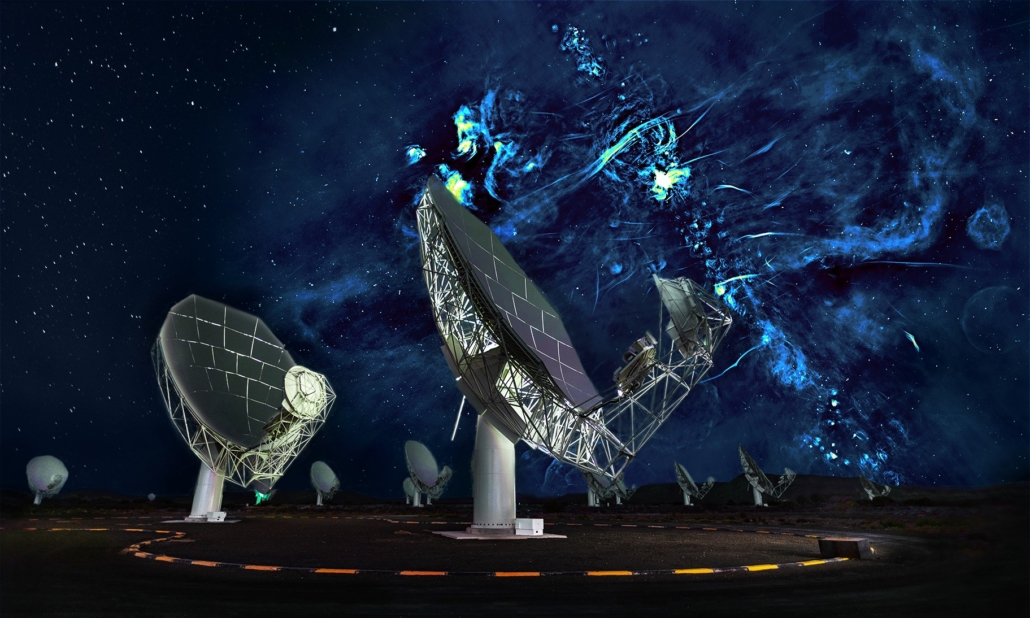
\includegraphics[width=12.3cm]{cover.jpg}}
}
\vspace{1.5cm}
\vspace{1.5cm}


\vfill
\author{Authors:  Telescope Operators}
\date{}


\begin{document}
\maketitle
 
\chapter*{}

\begin{table}[h]
		\textbf{\centerline{DOCUMENT APPROVALS}}

	\begin{tabular}[b]{|c|c|c|c|c|c|}
	\hline
	&	\textbf{Name}&	\textbf{	Designation}&		\textbf{Affiliation}&	\textbf{	Date}&		\textbf{Signature}\\
	\hline
	\textbf{Prepared By}&	Ops Team&	Operators&	SARAO&	&\\	
	\hline
	\textbf{Reviewed By}&	Ops Team&	Operators&	SARAO&	&	N/A\\
	\hline
	\textbf{Accepted By}&	C Gumede&	Telescope Operations& Manager&	&SARAO\\
	\hline
	\textbf{Approved By}&	L Magnus&	Head: Operations&	SARAO&&\\
	
	\hline
\end{tabular}	
\end{table}

\begin{table}[h]
	\textbf{\centerline{DOCUMENT HISTORY}} 

\begin{tabular}[b]{|c|c|c|c|}
	\hline
	{\fontsize{8}{3}\selectfont \textbf{Revision}}&{\fontsize{8}{3}\selectfont						\textbf{Date Of Issue}}&	\textbf{Prepared By}&	{\fontsize{8}{3}\selectfont	\textbf{Comments (e.g. ECN Number or changes to document)}}\\
	\hline			
{\fontsize{10}{4}\selectfont	A}	&{\fontsize{10}{4}\selectfont								12-04-2021}&	{\fontsize{10}{4}\selectfont Ops}&{\fontsize{10}{4}\selectfont	Issued for Comments} \& {\fontsize{10}{4}\selectfont Review}\\ 
	
	\hline
\end{tabular}
\end{table}
\begin{table}[h]


\textbf{\centerline{DOCUMENT DISTRIBUTION}} 
\begin{tabular}[b]{|p{15.5cm}|}
	\hline
	{\fontsize{10}{4}\selectfont Publish in eB and Distribute to all signatories on the document and the relevant line managers.}\\
	\hline
\end{tabular}
\end{table}

\begin{table}[H]

\textbf{\centerline{DOCUMENT SOFTWARE}} 

%\centering
\resizebox{\textwidth}{!}{%
	\begin{tabular}[b]{|p{2cm}|p{2cm}|p{2cm}|p{7.4cm}|}
	
	\hline
	
	\multicolumn{2}{|c|}{\textbf{Package}}	& \textbf{Version}	& \textbf{Filename}\\
	\hline
	Latex&TexStudio & 	N/A& \url{https://docs.google.com/document/d/1AOin8UJAxStFA71TCvOO4q_bQ_mOupbCd9ghWZxnRc/edit#} \\
	\hline
\end{tabular}

}
\end{table}

\textbf{\centerline{COMPANY DETAILS}} 
\resizebox{\textwidth}{!}{%
	\begin{tabular}[b]{|p{3cm}|p{4.1cm}|p{4.1cm}|p{4.1cm}|p{4.1cm}|}
		\hline
		
		Name & 
		SKA SA, Johannesburg Office
		(Rosebank, Gauteng)
		
		& 
		SKA SA, Cape Town Office
		(Pinelands, Western Cape)
		
		& 
		SARAO, HartRAO
		(Hartebeeshoek, Gauteng)&SARAO, Karoo Astronomy Reserve
		(Carnarvon, Northern Cape)   \\
		
		\hline
		
		Physical/Postal
		Address
		
		&
		1$^{st}$ Floor, 17 Baker Street 
		Rosebank, Gauteng
		2196, South Africa
		&
		
		3rd Floor, The Park,
		Park Road, Pinelands,
		7405, South Africa
		
		& 
		P.O.Box 443, Krugersdorp 1740, South Africa 
		
		&
		Posbus 69, Carnarvon, 8925, South Africa\\
		
		\hline
		
		
		Tel.&
		+27 11 268 3400&
		+27 21 506 7300&
		+27 (12) 301-3100&
		+27 21 506 7300\\
		
		\hline
		
		Fax.&
		27 11 442 2454&
		+27 21 506 7375&
		+27 (12) 301-3300&
		+27 (0)86 538 6836\\
		
		\hline
		Website&
		www.ska.ac.za&
		www.ska.ac.za&
		www.hartrao.ac.za&
		www.ska.ac.za\\
		\hline	
		
	\end{tabular}
	|}




 	\chapter*{}
{
\includegraphics[width=16cm]{logo2.png}}
\vspace{1cm}
\vspace{1cm}

{\color{red}\textbf{\centerline{MeerKAT Telescope Operator Manual}} }

{\color{red}\begin{tabular}[b]{p{8cm} R{7.6cm}}

	

	Document number&	SSA-0006D-003\\
	Revision&	A\\
	Classification&	Commercial in Confidence\\
	Prepared By	&Telescope Operators\\                              
	Approval Date &	01 02 2021\\
	

\end{tabular}
}
\vspace{1cm}
\vspace{1cm}
\vspace{1cm}

{\color{red}\begin{tabular}[b]{p{6cm}p{0.2cm}p{9cm}}
	
	\hline	
	
	Organisation&	:&
	NRF (National Research Foundation)\\
	Facility	&:&
	SARAO (South African Radio Astronomy Observatory)\\
	Project	&:&
	N/A\\
	Document Type	&:&
	Guidelines (UG)\\
	Function/Discipline&	:&
	Operations Management (0006)\\
	\hline
\end{tabular}
}

 
 \chapter*{Preface}

This manual is designed to help new users (i.e Students, Oservers) of the MeerKat Radio Telescope to understand basic operational procedures, and scientific procedures that are being used to carry out scientific observations.  The complexity of the instrument requires many software interfaces for instrument setup, scheduling, monitoring and maintenance management. \\

The document is an effort to explain the terminologies that are often used locally in operations and commissioning divisions of SARAO.  The scientific community is more interested in the scientific methods that were used to calibrate, validate and test all the critical components of the telescope. Thus,  important calibration  procedures are briefly described with reference to detailed documentation.



 \chapter*{Naming Convenctions }


 The following naming convections have been adopted for this manual:  
 \begin{itemize}
 	\item {} Scientific Units \cite{unit}.\\
 	 e.g \unit{dB}
 	\item {} Names of servers and computers. \\
    e.g	$<$\server{server}$>$.$<$\server{telescope}$>.<$\server{site}$>$\server{.kat.ac.za.}\\
 	 \server{kat@obs.mkat.karoo.kat.ac.za} 
 	\item {} Names of software packages.\\
 	e.g  \package{PYTHON}
 		
 	\item {} Terminal commands and program option. 	 e.g 
 	\begin{lstlisting}[style=DOS, tabsize=4]
 	ssh kat@obs.mkat.karoo.kat.ac.za
 	\end{lstlisting}
 	\item {} GUI commands e.g\\
 	Select \textbf{Links} $>$ \textbf{Grafana}  $>$ \textbf{Overview}
 	\item {} Folders and Filenames. e.g \file{image.py}
 	\item{} Names of Meerkat components. \\ 
 	e.g \component{m001}
 	\item{} Names of sensors. \\
 	  e.g  \sensor{ap.control}
 	
 	\item{} Scripts options and parameters \\
 	e.g  \option{fft-shift}
 	\item{} Links and urls \\
 	e.g  \url{fft-shift}
 		\item{} Progress, sensor and system logs  \\
% 	e.g  \output{16:32:39.386Z WARNING   - m063ht}
 \end{itemize}




	
	\chapter*{List of Acronyms}
	\addcontentsline{toc}{chapter}{List of Acronyms}
	
	\setlength{\LTleft}{0pt}
	
	\begin{longtable}{@{}ll@{}}
		ABL	&	Allocated Baseline	\\
		Ac	&	Critical Availability	\\
		ADR	&	Architecture Design Review	\\
		AGN	&	Active Galactic Nuclei	\\
		Ai	&	Inherent Availability	\\
		AOR	&	Annual Operating Requirement	\\
		AR	&	Acceptance Review	\\
		BOM	&	Bill Of Material	\\
		CA	&	Criticality Analysis	\\
		CDR	&	Critical Design Review	\\
		DDR	&	Detail Design Review	\\
		D-Level	&	Deport Level	\\
		DLM	&	Depot Level Maintenance	\\
		FAT	&	Factory Acceptance Tests	\\
		FMEA	&	Failure Modes and Effects Analysis	\\
		FMECA	&	Failure Modes, Effects and Criticality Analysis	\\
		FPGA	&	Field Programmable Gate Array	\\
		FRACAS	&	Failure Reporting and Corrective Action System	\\
		GHz	&	Giga Hertz	\\
		GUI	&	Graphical User Interface	\\
		HartRAO	&	Hartbeeshoek Radio Astronomy Observatory	\\
		Hrs	&	Hours	\\
		I-Level	&	Intermediate Level	\\
		ILM	&	Intermediate Level Maintenance	\\
		ILOR	&	Intended Learning Outcomes Report	\\
		ILS	&	Integrated Logistic Support	\\
		ISO	&	International Standards Organisation	\\
		KAT-7	&	Karoo Array Telescope, 7 array	\\
		Kg	&	Kilogram	\\
		Km	&	Kilometer	\\
		L3/4/5	&	Level 3/Level 4/Level 5	\\
		LEMP	&	Logistic Engineering Management Plan	\\
		LRU	&	Line Replaceable Unit	\\
		LSA	&	Logistic Support Analysis	\\
		MBL	&	Manufacturing Baseline	\\
		
		\\
		MSCDR	&	Media Selection \& Curriculum Development Report	\\
		MSP	&	Maintenance \& Support Plan	\\
		MTBCF	&	Mean Time Between Critical Failures	\\
		MTBF	&	Mean Time Between Failures	\\
		MTTRc	&	Mean Time To Repair Critical	\\
		MTTRi	&	Mean Time To Repair Inherent	\\
		NQF	&	National Qualification Framework	\\
		OEM	&	Original Equipment Manufacturer	\\
		O-Level	&	Organisational Level	\\
		OLM	&	Organisational Level Maintenance	\\
		OTLR	&	Operator Task List Report	\\
		PBL	&	Product Baseline	\\
		PBS	&	Physical Breakdown Structure	\\
		PC	&	Printed Circuit	\\
		PDR	&	Preliminary Design Review	\\
		PHS and T&Packaging, Handling, Storage and Transportation	\\
		PPPM	&	Preparation, Preservation, Packaging \& Marking	\\
		PPPR	&	Personnel Performance Profile Report	\\
		PRR	&	Production Readiness Review	\\
		PSS	&	Product Supplier Support	\\
		QBL	&	Qualification Baseline	\\
		RAM	&	Reliability, Availability, Maintainability	\\
		RBL	&	Requirements Baseline	\\
		Relc	&	Reliability Critical	\\
		Reli	&	Reliability Inherent	\\
		RF	&	Radio Frequency	\\
		RFI	&	Radio Frequency Interference	\\
		RM	&	Rotation Measures	\\
		RR	&	Requirements Review	\\
		RTS	&	Receptor Test System	\\
		S and TE	&	Support and Test Equipment	\\
		SAQA	&	South African Qualifications Authority	\\
		SEMP	&	System Engineering Management Plan	\\
		SKA	&	Square Kilometer Array	\\
		S-Level	&	Supplier Level	\\
		SLM	&	Supplier Level Maintenance	\\
		SNR	&	Supernova Remnants	\\
		SRU	&	Shop Replaceable Unit	\\
		TBD	&	To Be Determined	\\
		TRR	&	Test Readiness Review	\\
		TSR	&	Training Survey Report	\\
		TTLR	&	Technical Task List Report	\\
		vs	&	Versus	\\	
	\end{longtable}


 
% \section{A}
% 
% \acro{GEOAA}
% 
% \acro{IMO}
% 
% \acro{IMO}
% 
% \acro{GEOAA}
% 
% \acro{OP}
% 
% \section{B}
% 
% \acro{OP}
 
% \listofacronyms
 
 %\chapter*{Dedication}

% \renewcommand{\headrulewidth}{0.4pt}
% \renewcommand{\footrulewidth}{0.4pt}
% \chapter*{Declaration}
 
% \chapter*{Acknowledgements}
 
  \listoffigures
  \addcontentsline{toc}{chapter}{List of Figures}
%  \listoffigures\newpage.
% 
 
% \addtocontents{toc}{\protect\contentsline{chapter}{\listfigurename}{\getpagerefnumber{listoffigures}}}
% \addtocontents{toc}{\protect\contentsline{chapter}{\listtablename}{\getpagerefnumber{listoftables}}}
 
  
 \listoftables 
 \addcontentsline{toc}{chapter}{List of Tables} 
 \tableofcontents
 \chapter{Introduction}
 \section{Int}
see \textbf{Figure}:\ref{fig:three graphs}
\begin{figure}
	\centering
	\begin{subfigure}[b]{0.3\textwidth}
		\centering
		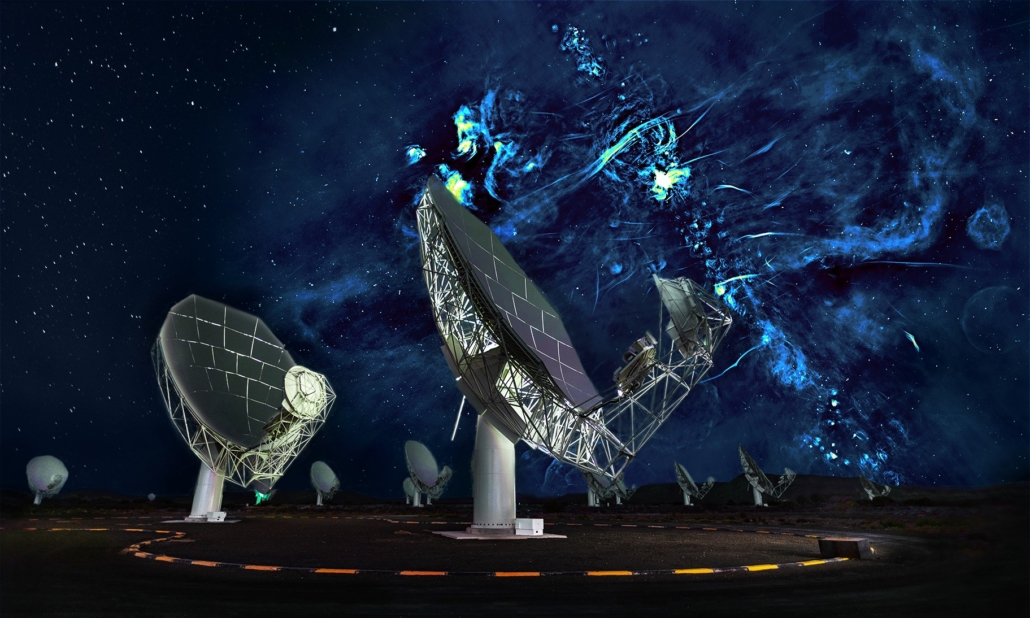
\includegraphics[width=\textwidth]{cover.jpg}
		\caption{$y=x$}
		\label{fig:y equals x}
	\end{subfigure}
	\hfill
	\begin{subfigure}[b]{0.3\textwidth}
		\centering
		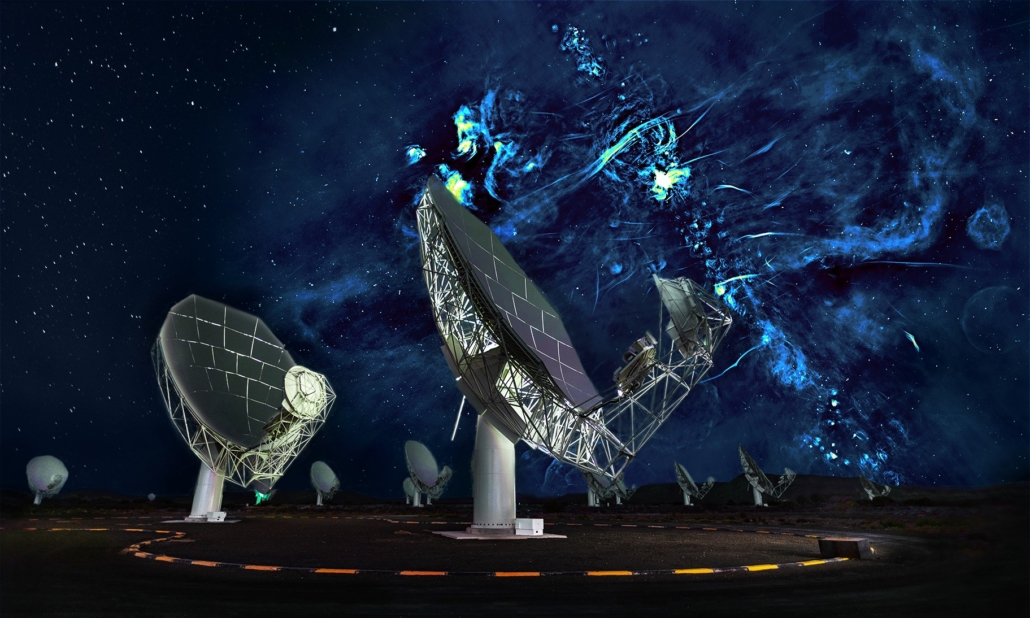
\includegraphics[width=\textwidth]{cover.jpg}
		\caption{$y=3sinx$}
		\label{fig:three sin x}
	\end{subfigure}
	\hfill
	\begin{subfigure}[b]{0.3\textwidth}
		\centering
		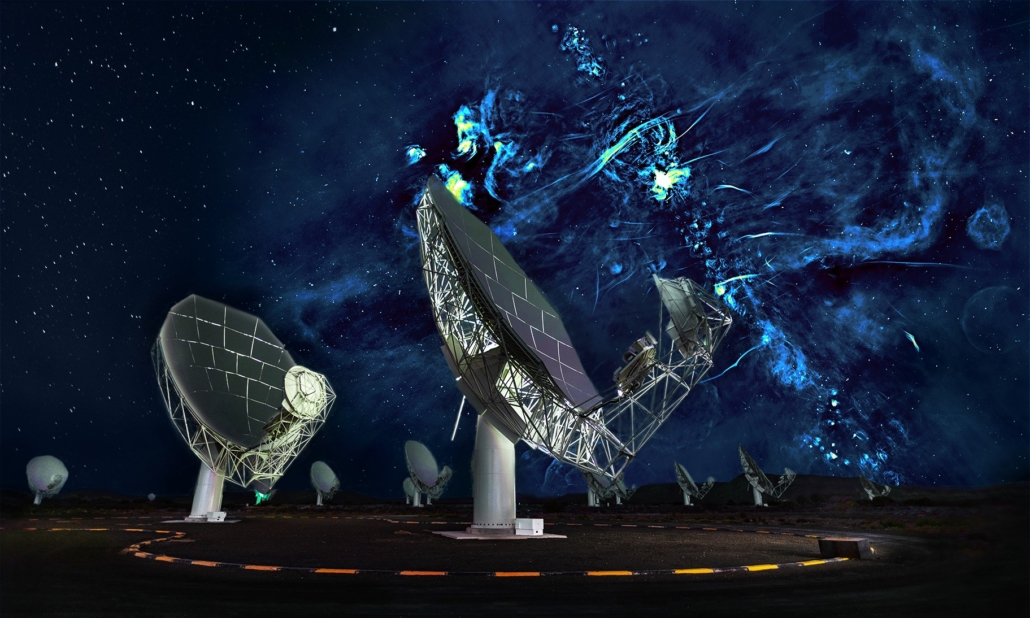
\includegraphics[width=\textwidth]{cover.jpg}
		\caption{$y=5/x$}
		\label{fig:five over x}
	\end{subfigure}
	\caption{Three simple graphs}
	\label{fig:three graphs}
\end{figure}

%  \chapter{Instrument Calibration Procedures}
% \section{Receiver System Tests (RTS) and Calibration}

\section{Cable Delay Calibration}
\subsection{Band Pass Calibration}
\section{Phase-up and Phase Down}
\section{Pointing Calibration}
\subsection{Single Dish Pointing}
\subsubsection{Pointing Check}
\subsubsection{Interfrometric Pointing}
\subsubsection{AP Motion Profilers}
\section{Holography Test}


\section{Digitiser attenuation levels}
\section{System Sychoronisation}

\subsection{Digitiser Master Controller}
\subsection{Digitiser Synchronisation}
\subsection{Aantenna Control Unit Synchronisation}



	
% 
%  \chapter{Safety Procedure}
% \section{ Operational Safety Procedure}

  \chapter{Logging into the system}
 
        The telescope system software runs on Linux servers and the basic understanding of the Linux operating system is required in order to operate the telescope. The Telescope Operator will also use Portal’s CAM graphical user interface referred to as GUI in order to interact with the telescope system. In order for anyone to interact with the telescope system, they need to have been given access via CAM portal.  The person needs a username and password to login into the system. When a person logs in for the first time on the system in order to control and monitor MeerKAT telescope system, the following is important to note. The system has many server nodes that are used for controlling and monitoring various parts of the system.  The most used servers nodes are:
        \begin{itemize}
\item{} \server{portal.mkat.karoo.kat.ac.za} and
\item{} \server{obs.mkat.karoo.kat.ac.za} 
\end{itemize}
The naming convention for the server nodes is always\\ $<$\server{server}$>$.$<$\server{telescope}$>.<$\server{site}$>$\server{.kat.ac.za.}, with :
\begin{itemize}
\item{} the first parameter is server node name
\item{} the second is the telescope (Currently: \server{mkat, kat7, mkat-rts}) and
\item{} the third is karoo for site systems different from lab systems.
\end{itemize}
\subsection{Portal Server}
The URL of where to find the GUI is \server{http://portal.mkat.karoo.kat.ac.za/}. 
The login details to the portal link above will be provided by CAM admistrator.
The landing page is as shown in \textbf{Figure}~\ref{fig:image71}. 
\clearpage
\begin{figure}[!thb]
	\centering
	%\includegraphicsdpi{100}{}{bur1.png}     
	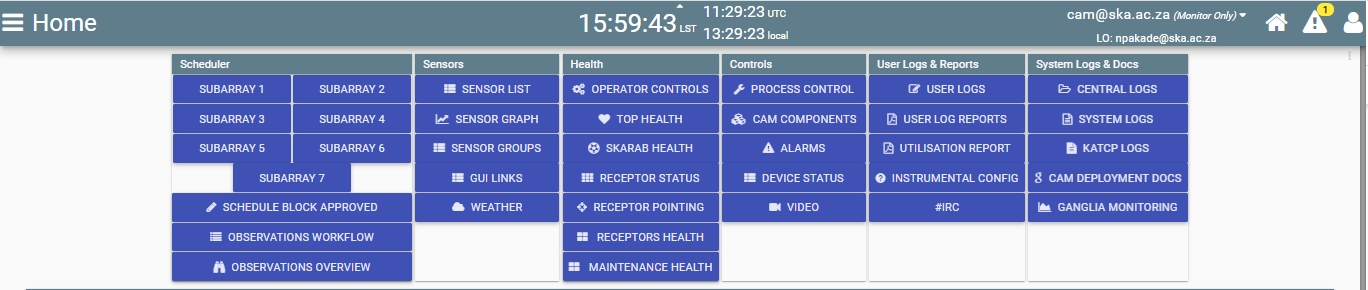
\includegraphics[scale=0.3]{Chapters/images/image71.png}
	
	%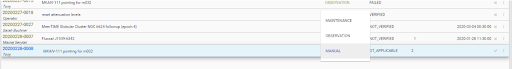
\includegraphics[resolution=100]{bur1.png}
	\caption{CAM GUI home page}
	\label{fig:image71}
\end{figure}




This will allow one to monitor the telescope system but will not be able to control the system. The person will have to be given the lead operator role (LO) or expert role in order to control the telescope for safety reasons. This page will allow one to access different functionality of the telescope system, monitoring and control i.e. if for instance one is interested in building and running subarray 1, the configuring of a subarray, one will click and open “SUBARRAY1 tab. This page will be shown as in \textbf{Figure}~\ref{fig:image38} below.

\begin{figure}[!thb]
	\centering
	%\includegraphicsdpi{100}{}{bur1.png}     
	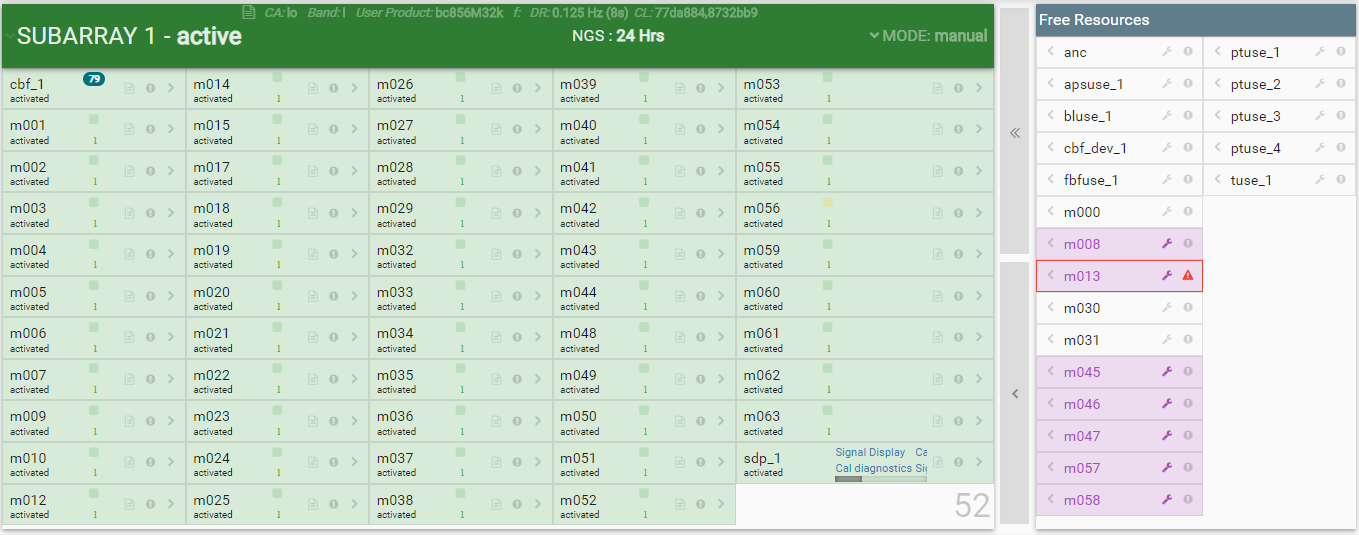
\includegraphics[scale=0.3]{Chapters/images/image38.png}
	
	%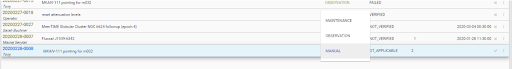
\includegraphics[resolution=100]{bur1.png}
	\caption{CAM GUI Subarray1 window}
	\label{fig:image38}
\end{figure}




In order to learn more about the GUI and the telescope system, the user must familiarise with different tabs on the GUI. More information will be discussed in the following sections of this document. 

\subsection{Obs Server/Machine}
The node server \server{“obs.mkat.karoo.kat.ac.za”} allows interaction with the live system via the command line and ipython interface. This is where the instructions to create a schedule block SB is provided.The user is required to command the telescope in the Linux environment from the command line using Linux and python commands. 
\clearpage
The user will be given credentials to login into the server. The server node to login using ssh command is \server{“obs.mkat.karoo.kat.ac.za” } and this will open up a page as shown in \textbf{Figure}~\ref{fig:image87}.

%\begin{figure}[!thb]
%	\centering
%	%\includegraphicsdpi{100}{}{bur1.png}     
%	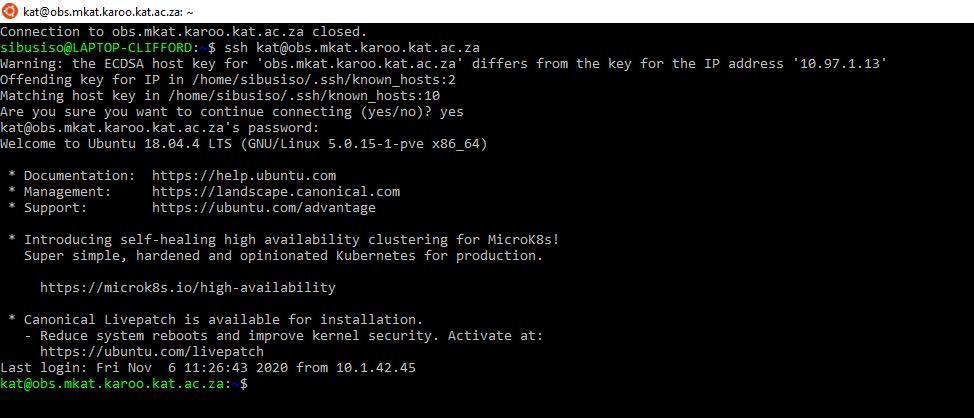
\includegraphics[scale=0.45]{Chapters/images/image87.png}
%	
%	%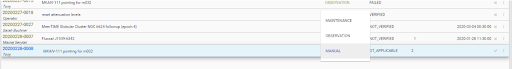
\includegraphics[resolution=100]{bur1.png}
%	\caption{Terminal ssh login to obs machine}
%	\label{fig:image87}
%\end{figure}
\begin{figure}[!thb]
	\centering
	%\includegraphicsdpi{100}{}{bur1.png}     
	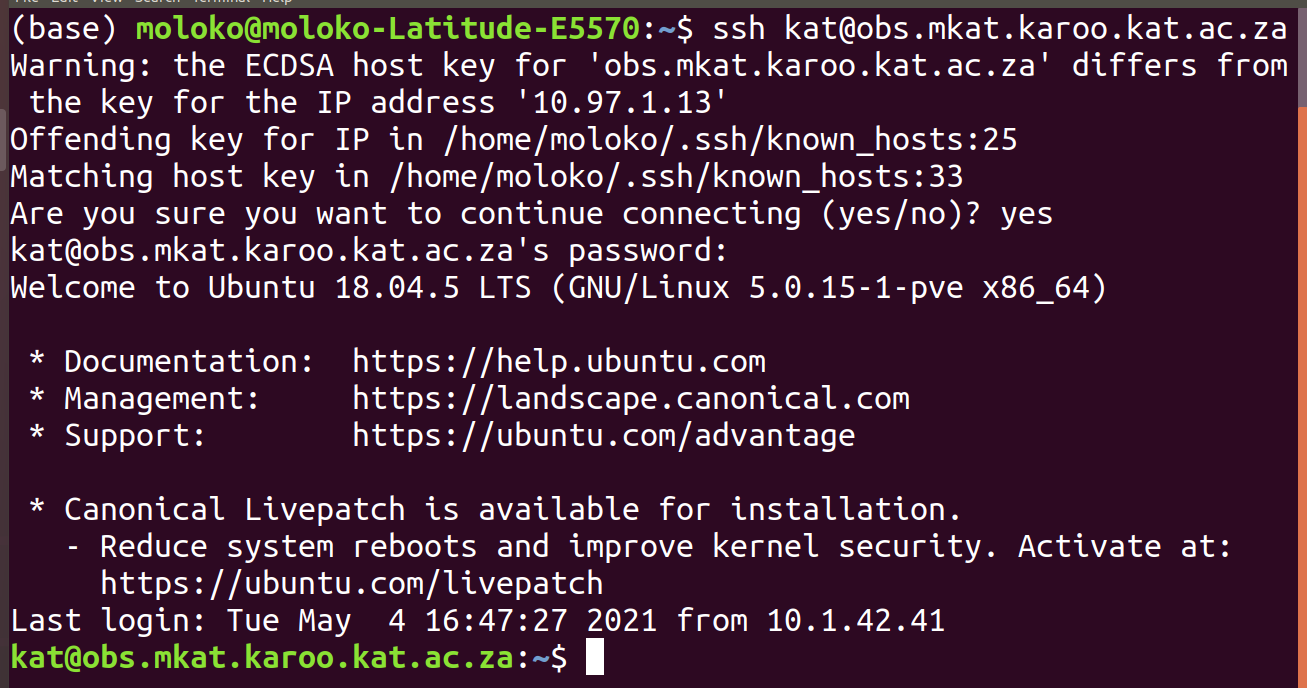
\includegraphics[scale=0.33]{Chapters/images/terminal.png}
	
	%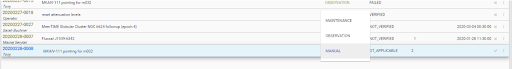
\includegraphics[resolution=100]{bur1.png}
	\caption{Terminal ssh login to obs machine}
	\label{fig:image87}
\end{figure}
 
 

 
 \chapter{Handover Procedures}
  

The telescope can only be controlled by a lead operator who has the correct credentials. To be a lead operator you will have credentials to control and monitor the telescope and these credentials are supplied by the Telescope Operations Manager. The telescope operates 24 hours a day, 7 days week and 365 days a year and there are 3 shifts a day split over 8 hours each. During the shift we have a lead operator who is responsible for controlling and monitoring the telescope system. Therefore there are three operators over a 24 hour period configuring and monitoring the telescope system at all times. Between the shifts one lead operator  hands over the system to the next operator. The paragraphs below describe in detail the procedure begging followed during the handover process.  
\section{Operator Handover Procedures}
Each Operator during the shift compiles a list or record  of the incidents that occured during  shift.  This record is called a handover document and this is different from the operations meeting minutes. The operator will update the incoming lead operator and also give this document to the next lead operator and this document will contain but not limited to this information below:
\begin{itemize}
\item{} What is currently being done with the telescope?
\item{} What observation is coming up after the current one?
\item{} What receptors are available and what receptors are expected back from maintenance?
\item{} What resources have been booked out for. maintenance and when - who to contact to get them back?
\item{} What problems are currently opened under which subsystems - supplement? this with reading open-ended user logs and the checklist [\textbf{Appendix A}]"
\item{} What are the problems experienced and what does the incoming operator need to look out for?
\end{itemize}
\section{Booking resource for maintenance}
The lead operator during the morning shift will be required to make resources (AP, Receivers, Digitiser, CBF etc) available to site technicians and engineers to conduct maintenance and upgrades. The resources will normally be booked for maintenance or upgrade at least a day before unless the resource is in error and cannot be used for operations. The lead operator will follow the process below:
\begin{itemize}
\item{} Check for booking in the Engineering Spreadsheet or Site calendar.
\item{} Mark the resource to maintenance - a log is automatically opened in the user logs. Add reason for booking in the log.
\item{} If the resource booked causes system downtime, add the ‘timeloss’ tag to the user log for system utilisation statistics reporting.
\item{} Alert maintenance staff or engineering staff after the resources have been made available. 
\item{} This information must also be added in the handover document. 
\end{itemize}
\section{ Receiving a resource after maintenance or an update}
\begin{itemize}
\item{} During the handover, check the control status of the resource \sensor{ap.control} sensor in sensor list  as shown in \textbf{Figure}~\ref{fig:image98}.

 \begin{itemize}
\item[$\circ$] If it is in remote - usable
\item[$\circ$] If it is in local/manual/e-stop - must be reset by technician
\end{itemize}

\begin{figure}[!thb]
	\centering
	%\includegraphicsdpi{100}{}{bur1.png}     
	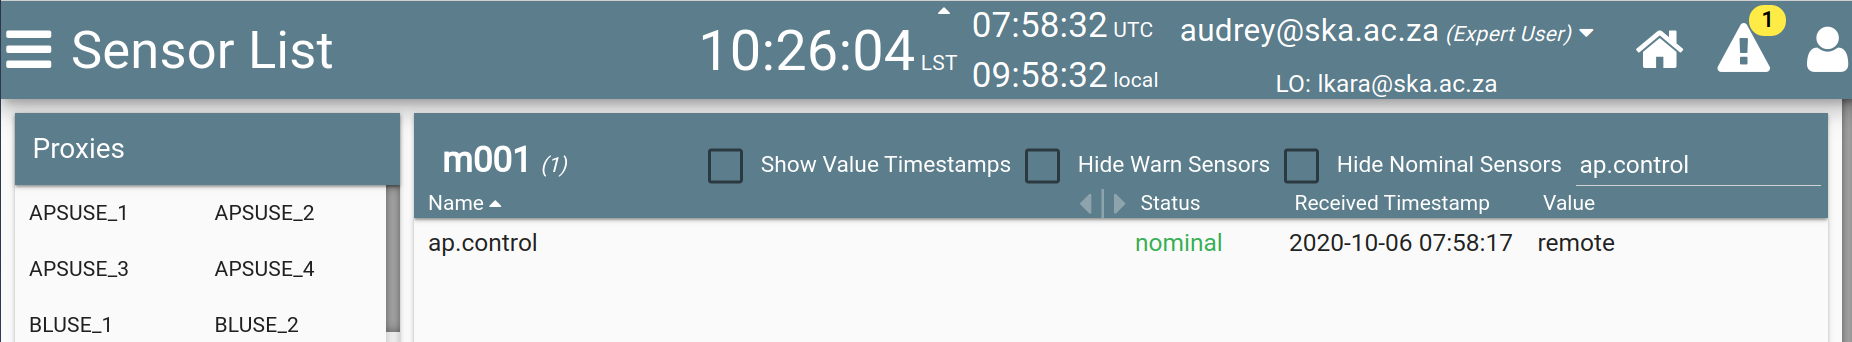
\includegraphics[scale=0.25]{Chapters/images/image98.png}
	
	%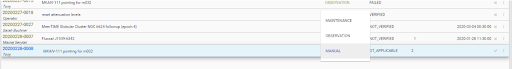
\includegraphics[resolution=100]{bur1.png}
	\caption{CAM GUI sensor list filtered with "Control"}
	\label{fig:image98}
\end{figure}
\item{} If in remote, check the health of the resource in detail

\begin{lstlisting}[style=DOS]
ssh kat@obs.mkat.karoo.kat.ac.za
./katsdpscripts/utility/check_ant.py --observer name --ant m0xx --proposal-id 22

\end{lstlisting}

Or 
\begin{lstlisting}[style=DOS]
./usersnfs/tiyani/meerkat_status.py --receiver rxl     

\end{lstlisting} (For L-band receivers)
\begin{lstlisting}[style=DOS]

./usersnfs/tiyani/meerkat_status.py --receiver rxu     

\end{lstlisting}
 (For UHF receivers)


\item{} Include the AP in the next observation to check signal quality
\item{} If a number of antennas are returning from maintenance and there is time before the next observation, create a small subarray with at least 4 antennas and run delay calibration, if there are less than 4 antennas available, build a subarray with those antennas but run three calibration script to check signal health.
\item{} Update OPS Catalyst page with correct number of APs available for use.

\section{Integrating a Receptor into Meerkat}
This must be done when an antenna has been in maintenance for an extended period of time or it was handed over to MPI for testing

Verify with the person who took the AP if they have changed anything in the digitiser,receiver or any other component configuration.
If there were changes made, talk to CAM to change what has been changed before testing the AP.
Run the \file{"check\_ant.py”} script as in the step above in 6.2
Mark the digitiser ready 
\begin{lstlisting}[style=DOS]
ssh kat@obs.mkat.karoo.kat.ac.za
ipython			
import katuilib
configure_cam("camcam","all")
cam.m0xx.sensor.dig`_selected_band.get_value()
cam.m0xx.req.digitiser_ready('l', timeout=60)
cam.m0xx.req.dig_select_band('l', timeout=60)
\end{lstlisting}




Where \component{m0xx} represents a receptor number e.g \component{m001}

\item{} Sync the digitiser using global sync - see next chapter.
\item{} Check the remaining hours left before the next global sync in sensor list of the CAM GUI as shown in \textbf{Figure}~\ref{fig:image68}.


\begin{figure}[!thb]
	\centering
	%\includegraphicsdpi{100}{}{bur1.png}     
	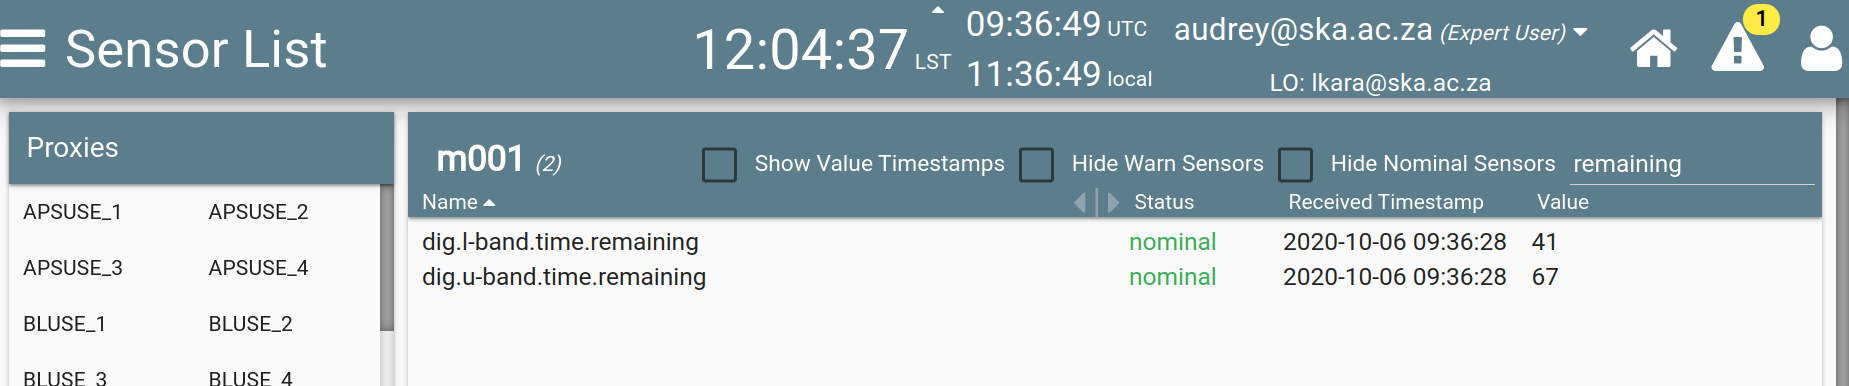
\includegraphics[scale=0.25]{Chapters/images/image68.png}
	
	%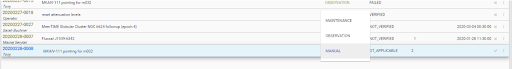
\includegraphics[resolution=100]{bur1.png}
	\caption{CAM GUI sensor list filtered by "remaining".}
	\label{fig:image68}
\end{figure}

These values above (41 \& 67) will indicate if global sync was successful or not for L and UHF$-$band digitisers.

\item{} Include the antenna in an array and run a calibrated delay script and see if it finds a solution. 
\begin{itemize}
\item [$\circ$] Look at the progress output of the delay cal script if the delay solutions are found.
		\item [$\circ$] During observation, look at the waterfall plot(signal displays) to see if there is a constant colour on its baseline. If the antenna looks noisy as in \textbf{Figure}~\ref{fig:image34} or has a rainbow, ask AoD to check its delay models.
\end{itemize}
 

\begin{figure}[!thb]
	\centering
	%\includegraphicsdpi{100}{}{bur1.png}     
	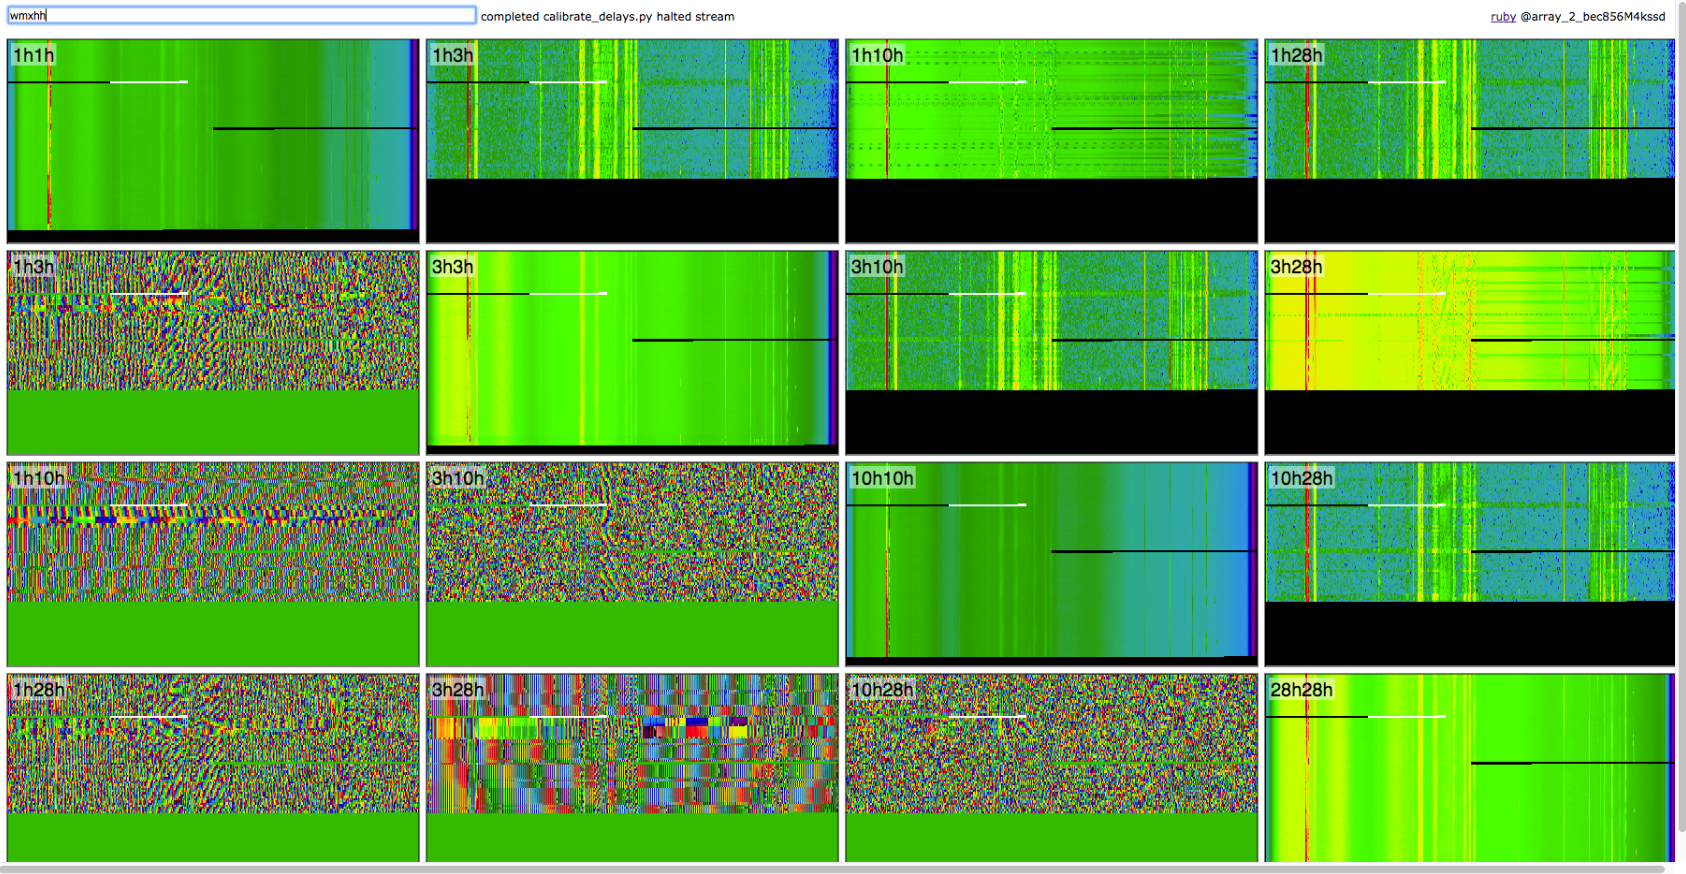
\includegraphics[scale=0.25]{Chapters/images/image34.png}
	
	%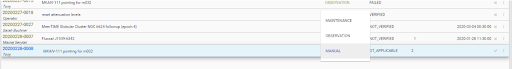
\includegraphics[resolution=100]{bur1.png}
	\caption{SDP waterfall plot.}
	\label{fig:image34}
\end{figure}

\item{} Before including the antenna in a Science observation communicate with the AoD about:
\begin{itemize}
	\item [$\circ$] interferometric pointing and notify operators to update pointing and delay models.
\end{itemize}

\item{} Update the Engineering Meerkat spreadsheet in the Owner tab.
\item{} Update the associated jira if necessary and close it.
\end{itemize}
 \chapter{System Settings Procedures}
 


\section{Moving Skarabs}


\textbf{WARNING}:\textit{ do not try to move the skarabs right after stopping or starting a subarray. The SKARABs need a couple of minutes to restart. Otherwise, they will not be found by the script, and will be left behind on the unwanted cmc.}\\

\subsection{CMC IP addresses}
The IP addresses for different machines are:
\begin{itemize}


	\item[] \server{cmc1: 10.103.254.1} and name: \server{cmc1.cbf.mkat.karoo.kat.ac.za}
\item[] \server{cmc2: 10.103.254.3} and name: \server{cmc2.cbf.mkat.karoo.kat.ac.za}, 

\item[] You can use the IP addresses or hostnames interchangeably (whichever you prefer) 


\item[] The cbf\_support repository is on git. You can clone it from:\\
git clone \url{https://github.com/ska-sa/cbf_support}
\end{itemize}
\subsection{Check the number of SKARABS}
In order to check the number if SKARABS are available in the CMC use the following
commands on the obs machine before attempting to move them. There should be about 220(as at 2020-01-06, but more will come) if they were all moved. If there are less, wait a couple
of minutes for them to restart.

\begin{lstlisting}[style=DOS]
kcpcmd -t 10 -s cmc1.cbf.mkat.karoo.kat.ac.za:7147 resource-list | grep "up$" | wc -l
\end{lstlisting}
(this will give you the number of skarabs available on cmc1.) 
\begin{lstlisting}[style=DOS]
kcpcmd -t 10 -s cmc2.cbf.mkat.karoo.kat.ac.za:7147 resource-list | grep "up$" | wc -l
\end{lstlisting}
(this will give you the number of skarabs available on cmc2.) \\

\subsection{Moving SKARABS}
If moving to cmc1 use -m cmc1:
\begin{lstlisting}[style=DOS]
./usersnfs/cbf_support/./cmc_manage_skarabs.py -m cmc1 -a 5 6 7 8 9 10 11 12 13 14 15 16 17 18 
 -k cmc1 cmc2
\end{lstlisting}
If moving to cmc2 use -m cmc2:
\begin{lstlisting}[style=DOS]
./usersnfs/cbf_support/./cmc_manage_skarabs.py -m cmc2 -a 5 6 7 8 9 10 11 12 13 14 15 16 17 18  -k cmc1 cmc2
\end{lstlisting}




This will connect to all the switches, discover which skarabs are currently online on the various ports, and move them to the requested master controller (-m switch).



\section{Global Synchronisation}

This script seeks to synchronize all digitisers to the Digitiser Master Controller so that signal/data coming into the correlator is in sync and correlates. 
\begin{itemize}
\item{} Ensure epoch sync on all usable digitisers (all bands) is done for the day
\item{} In the GUI, verify that all subarrays are inactive:
\begin{lstlisting}[style=DOS]
ssh kat@obs.mkat.karoo.kat.ac.za
run /home/kat/katsdpscripts/utility/global_sync.py
--observer= name --proposal-id=OPS-23

\end{lstlisting}



\item To check that all digitisers are synced and have the same epoch time, in the
same ipython session
\begin{lstlisting}[style=DOS]
ipython
import katuilib
configure()
kat.report_sensors('epoch','all')
\end{lstlisting}

\item Three ways to check time remaining for the next global sync
\begin{itemize}


\item [$\circ$] Check the Next Global Sync from the active subarray in the GUI (see \textbf{Figure}~\ref{fig:image115}). This gives
indication on what is the time remaining before the next global sync is
done.
\begin{figure}[H]
	\centering
	%\includegraphicsdpi{100}{}{bur1.png}     
	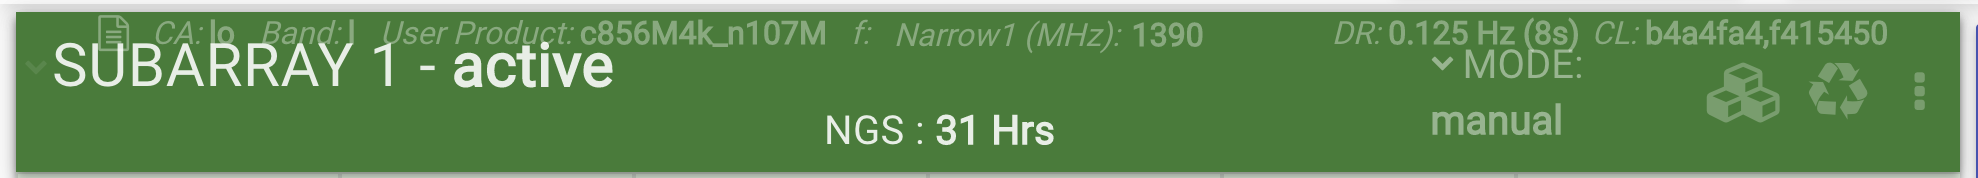
\includegraphics[scale=0.46]{Chapters/images/image115.png}
	
	%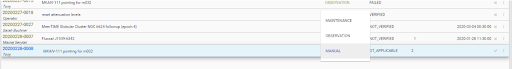
\includegraphics[resolution=100]{bur1.png}
	\caption{Global sync time remaining alert on the GUI }
	\label{fig:image115}
\end{figure}
\item [$\circ$] From the sensor list by typing \sensor{remaining} as shown in \textbf{Figure}~\ref{fig:image121}.
\begin{figure}[H]
	\centering
	%\includegraphicsdpi{100}{}{bur1.png}     
	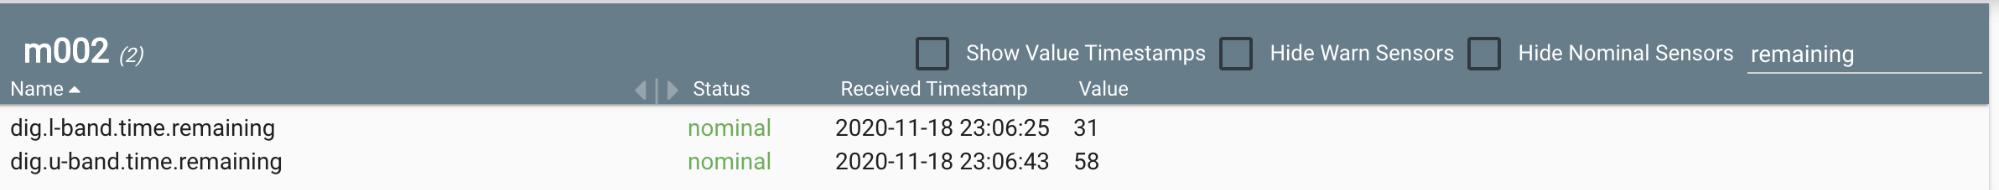
\includegraphics[scale=0.23]{Chapters/images/image121.png}
	
	%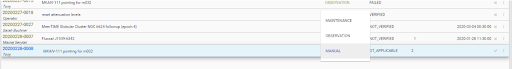
\includegraphics[resolution=100]{bur1.png}
	\caption{Global sync time remaining alert in sensor list}
	\label{fig:image121}
\end{figure}
\item [$\circ$] On IRC there is a reminder that reminds when to run a Global sync counting down
hourly from 15 hours left .
\end{itemize}
\end{itemize}


\section{Setting up digitisers}
\subsection{ Configured Ipython Session}
\begin{lstlisting}[style=DOS]
ssh kat@obs.mkat.karoo.kat.ac.za
ipython
import katuilib
configure_cam('camcam', 'all')
\end{lstlisting}

\subsection{ Mark Digitiser Absent}
The digitiser will be marked absent if there is maintenance work on the AP which
may cause the power to be switched off to the digitiser. It is also recommended that it
is marked absent if the AP will be out for maintenance for a long time.
In a configured ipython session run the following commands:
\begin{lstlisting}[style=DOS]
cam.m0xx.req.dig_select_band('0')
cam.m0xx.req.digitiser_absent('l', timeout=60)
\end{lstlisting}

In this case ‘l’ represents L-band digitiser
\subsection{Mark digitiser ready}
When the digitiser was marked absent or the new digitiser was installed in the AP, it
is required that it must be set ready for operations. Still in a configured ipython
session run the following commands:
\begin{lstlisting}[style=DOS]
cam.m0xx.sensor.dig_selected_band.get_value()
cam.m0xx.req.digitiser_ready('l', timeout=60)
cam.m0xx.req.dig_select_band('l', timeout=60)
\end{lstlisting}

If all digitisers were marked absent previously, this command above must be run for
all different bands, i.e. 'l' must be replaced with ‘u’ for UHF band digitiser. There is
no need to set an S-band digitiser at this stage.
\section{ Requesting which receptors have UHF$-$band digitisers}
In order to determine which antennas have UHF band digitisers installed on them, you will
run the following commands:
On the machine: ssh kat@obs.mkat.karoo.kat.ac.za and run the following commands.
\begin{lstlisting}[style=DOS]
u=`kcpcmd -t 60 -s 10.103.254.2:7147 list-digitisers | grep "u as
ready" | cut -d ' ' -f 2` && echo $u
\end{lstlisting}
If you prefer a list format do the following:
\begin{lstlisting}[style=DOS]
u=`kcpcmd -t 60 -s 10.103.254.2:7147 list-digitisers | grep "u as
ready" | cut -d ' ' -f 2` && echo -e "\n$u\n"
\end{lstlisting}


\section{ Digitiser Health}
In order to see the status of each digitiser that is operational one can use the following
commands to check for errors and health of each digitiser.
For L-band:
\begin{lstlisting}[style=DOS]
kat@obs.mkat.karoo.kat.ac.za:~$ dig-stats
\end{lstlisting}
For U-band:
\begin{lstlisting}[style=DOS]
kat@obs.mkat.karoo.kat.ac.za:~$ dig-stats 10.103.254.2:7147 u
\end{lstlisting}

\section{ Power sensors}
Important digitiser sensors to note for operations are power level The digitiser receives RF
signals from the receiver and the levels are measured at the inputs of the digitiser by the
RFCU. From the CAM GUI sensor list, filter for rfcu i.e. rfcu.*.power.  \textbf{Figure}~\ref{fig:image83} shows the power levels for each polarisation of m006.
\begin{figure}[H]
	\centering
	%\includegraphicsdpi{100}{}{bur1.png}     
	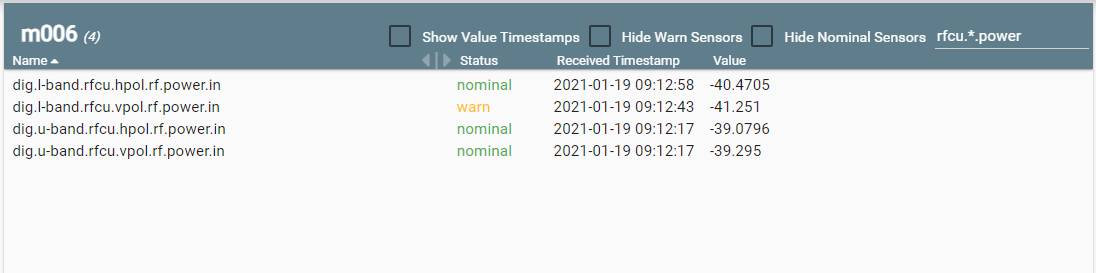
\includegraphics[scale=0.39]{Chapters/images/image83.png}
	
	%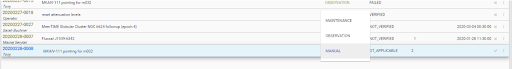
\includegraphics[resolution=100]{bur1.png}
	\caption{Global sync time remaining alert in sensor list}
	\label{fig:image83}
\end{figure}
The power levels for inputs on the L-band should be between -42dBm and -45dBm (when
not observing) and if they exceed these values this will be shown as warning. Low power
may mean that the LNA on the receiver are switched OFF or high power might mean AP is
pointing at a strong source or ground.\\

The second power level sensors for the digitisers are the ADC power levels which are
measured at the input of the ADC after the gains have been applied. The gains depends on
the attenuation levels which can be manually set, but we use separate scripts in setting and
refining attenuations. This is important to configure the attenuations so that all antennas
have the same output power levels. From the CAM GUI sensor list, filter for adc power i.e.
adc.*.power.in. \textbf{Figure}~\ref{fig:image51} shows the power levels for each polarisation of m006.
\begin{figure}[H]
	\centering
	%\includegraphicsdpi{100}{}{bur1.png}     
	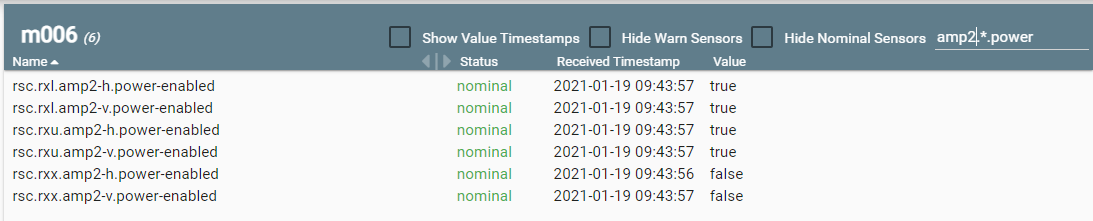
\includegraphics[scale=0.4]{Chapters/images/image51.png}
	
	%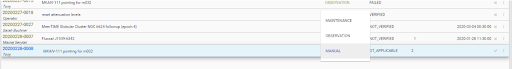
\includegraphics[resolution=100]{bur1.png}
	\caption{Global sync time remaining alert in sensor list}
	\label{fig:image51}
\end{figure}
It is recommended that the refine attenuations script should be run after building a new
subarray and the set attenuations script be run if there is a change in the signal chain i.e. a
Receiver or a Digitiser was replaced.
\section{ Updating config for a replaced digitiser}
Digitisers normally have their config files updated before they are handed over to
Operations. If a digitiser is replaced, it's serial number needs to be updated in CAM's
katconfig configuration files. This will require someone from the operations team to perform
github updates. The procedure to do that is shown below.\\

Note: Swaps done in S-band does not need updates in katconfig, because S-band
packetisers don’t use serial numbers, but instead use IP addresses according to the receptor number which gets set in the packetiser itself during installation.  This is their way
of communicating with MeerKAT. Hence the IP address never has to change when S-band
packetisers are replaced.
There are two different procedures which you can choose to follow:
\subsection{ On the terminal}
\begin{lstlisting}[style=DOS]
ssh kat@ops.kat.ac.za
cd katconfig/static/antennas/
git checkout master
git pull
git checkout karoo
git pull
git checkout -b update_m0XX_dig_config
\end{lstlisting}

If the response is:
\begin{lstlisting}[style=DOS]
fatal: A branch  named update\_m0XX\_dig_config already exists.
\end{lstlisting}
then rerun the command, but exclude “-b” this time.
\begin{lstlisting}[style=DOS]
git branch
\end{lstlisting}
 This should give: \option{*update\_m0XX\_dig\_config} 
\begin{lstlisting}[style=DOS]
ls
vi m0XX.conf 
\end{lstlisting}
(you can also use \option{nano m0XX.conf} whichever you comfortable with)

Type the letter “i” in order to edit the file.
The file format should be for example:
\begin{lstlisting}[style=DOS]
digitiser_l = ready:dig-041
\end{lstlisting} 
(we want to change this to the new serial number, i.e 064 for
example, to have \option{digitiser\_l = ready:dig-064})


any digitisers not installed should be of the format: 
\begin{lstlisting}[style=DOS]
digitiser_x = absent
\end{lstlisting}
Save the file and exit (press Esc, then type ":wq!")

\begin{lstlisting}[style=DOS]
git diff (shows changes you have made, check they are correct)
git add .
git commit -m "Updating (relevant band) digitiser serial no to 0XX on
m0XX"
git push --set-upstream origin update_m0XX_dig_config
\end{lstlisting}
\subsection{ On Github website}
\begin{itemize}


\item  Go to github:  \url{https://github.com/ska-sa/katconfig}
\item  Go to the new branch by clicking  on the dropdown list on available branches as shown in \textbf{Figure}~\ref{fig:image83} 
(should currently be on the karoo branch) and then selecting the branch name
of the new branch created .
\begin{figure}[H]
	\centering
	%\includegraphicsdpi{100}{}{bur1.png}     
	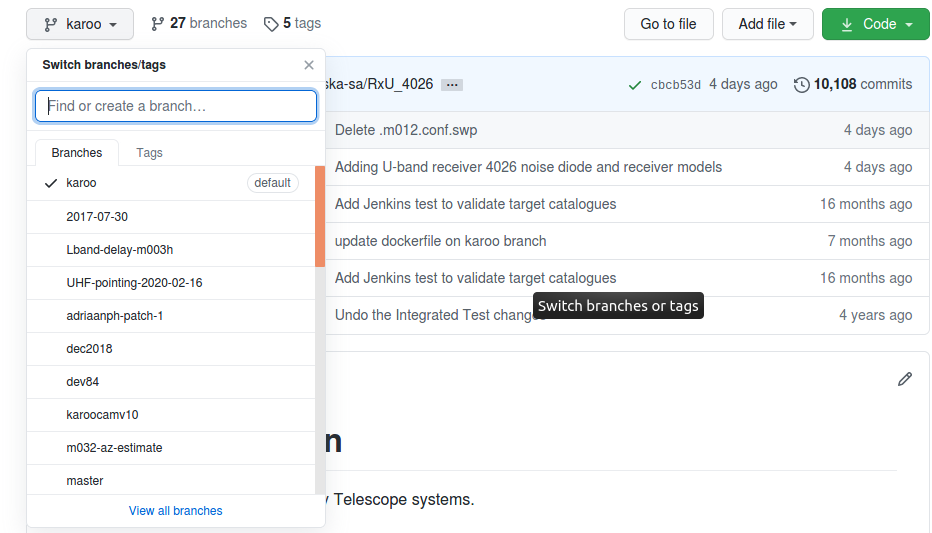
\includegraphics[scale=0.43]{Chapters/images/image108.png}
	
	%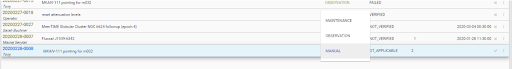
\includegraphics[resolution=100]{bur1.png}
	\caption{Github new branch select}
	\label{fig:image108}
\end{figure}

\item Create pull request from \option{update\_m0XX\_dig\_config} (name of branch created)
to karoo by clicking on “Pull request” at the top right as shown in \textbf{Figure}~\ref{fig:image73}.
\begin{figure}[H]
	\centering
	%\includegraphicsdpi{100}{}{bur1.png}     
	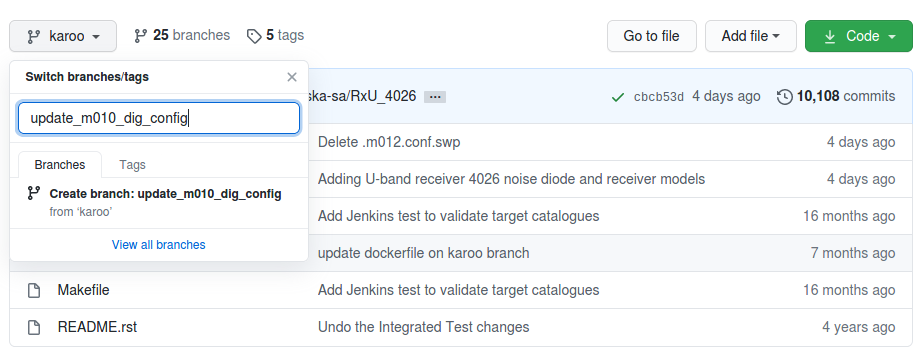
\includegraphics[scale=0.43]{Chapters/images/image73.png}
	
	%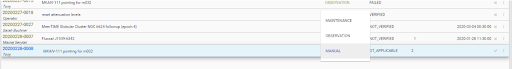
\includegraphics[resolution=100]{bur1.png}
	\caption{Github create pull request }
	\label{fig:image73}
\end{figure}



\item Make sure \option{base:karoo} and \option{compare:update\_m0XX\_dig\_config} is
selected. (Also make sure it’s only the files you have modified which are part
of the pull request - if you did the above steps properly that will be the case).
\item Then write a comment stating what you are doing, why (give Jira number if
applicable) and make the request out to Pieter Kotze. See an example in \textbf{Figure}~\ref{fig:image47}.
\begin{figure}[H]
	\centering
	%\includegraphicsdpi{100}{}{bur1.png}     
	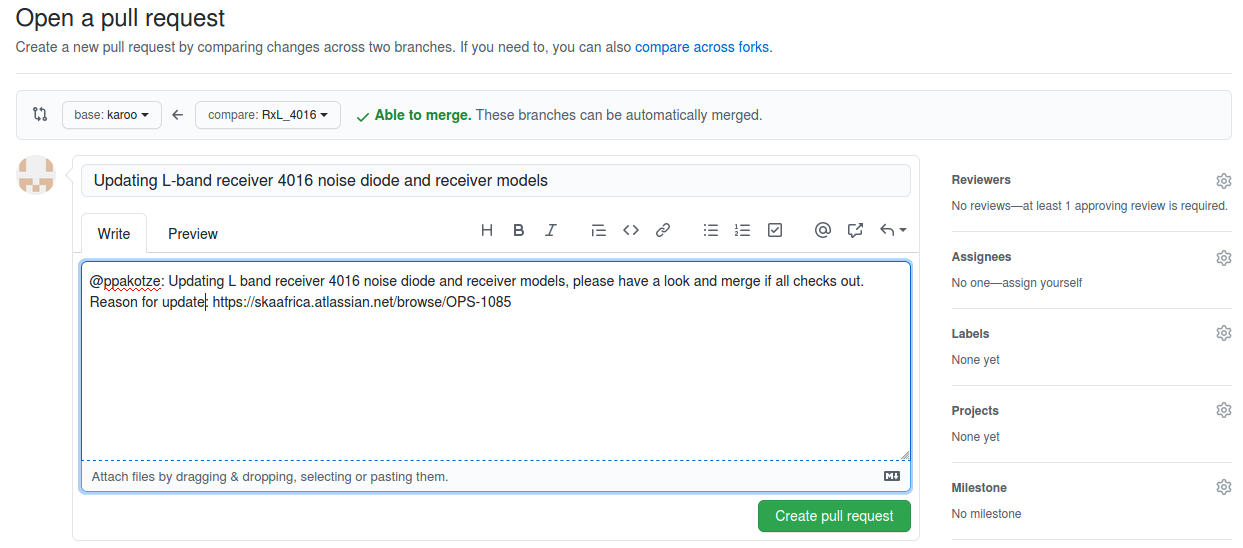
\includegraphics[scale=0.33]{Chapters/images/image47.png}
	
	%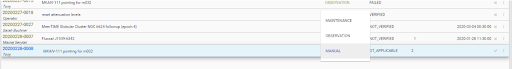
\includegraphics[resolution=100]{bur1.png}
	\caption{Github open pull request }
	\label{fig:image47}
\end{figure}
\item At the right hand side at the top next to “Reviewers”, click on the gear icon. It
will drop down a list of reviewers to choose from. Type “ppakotze” (see \textbf{Figure}~\ref{fig:reviewers}) in the
search field to find Pieter K and then click on Pieter K to request him to
approve your pull request (It will show a check mark next to his name, and
then under “Reviewers” you will see a yellow dot next to his name).

\begin{figure}[H]
	\centering
	%\includegraphicsdpi{100}{}{bur1.png}     
	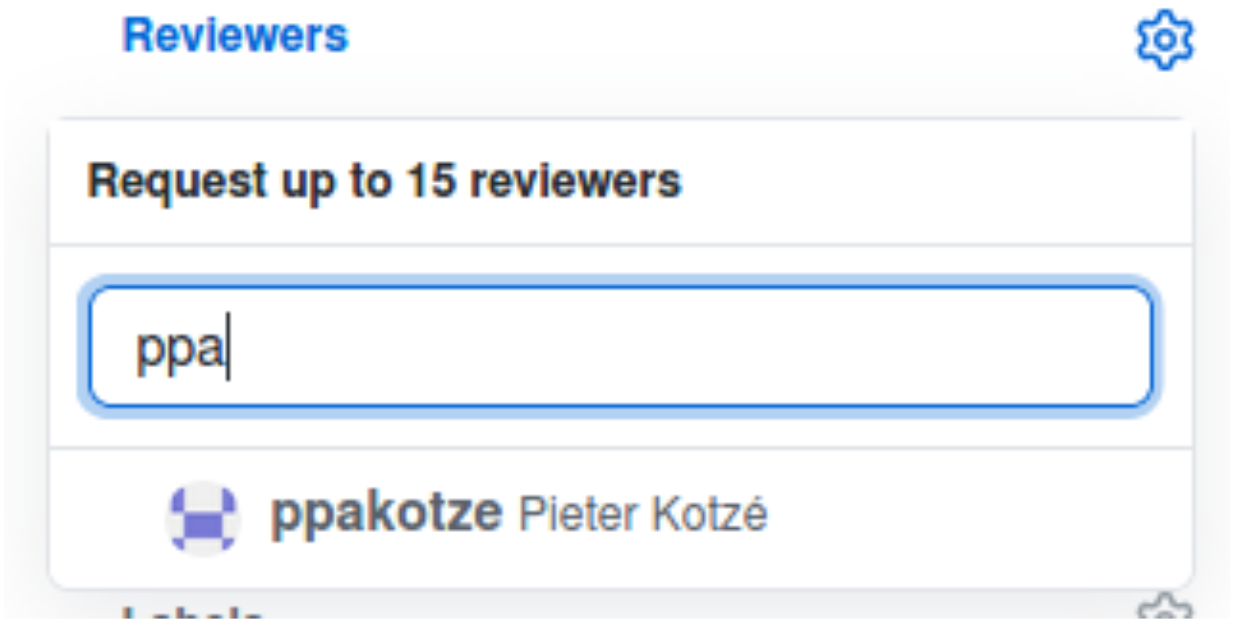
\includegraphics[scale=0.26]{Chapters/images/reviewers.png}
	
	%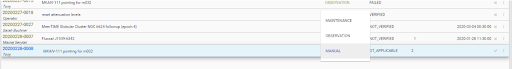
\includegraphics[resolution=100]{bur1.png}
	\caption{Github revievers dialogue }
	\label{fig:reviewers}
\end{figure}
\item Then click on “Create pull request”.\\
\textit{ Note: After Pieter K approves the pull request, he usually also merges
the pull request, but sometimes you have to do the merging yourself.
You do this by going to the pull request after it has been approved,
and then click on “Merge pull request” at the bottom and then “Confirm
merge”}
\end{itemize}






	
 
 
 \chapter{Receiver Systems}
 \section{Positioning the Receiver Indexer}

Receiver Indexer (RI) carousel has four defined positions for each of the receivers it hosts. By selecting the frequency band on CAM’s  GUI during building of a subarray you are selecting a receiver position mounted on the indexer. Currently we are using L-band and UHF-band for observations and S-band is still being integrated. The raw angles for receivers when they are indexed are:
\begin{itemize}
\item{} L band = 40deg
\item{} X band = 80deg
\item{} U band = 120deg
\item{} S band = 0deg
\end{itemize}

There is no X$-$band receiver installed and X$-$band position is used for parking antennas for the flight arrival and departure on site. 

In order to index the receiver to be used for the observation, On the \server{obs} machine \server{obs.mkat.karoo.kat.ac.za},  run
\begin{lstlisting}[style=DOS]
ipython
Import katuilib
configure_cam('camcam', 'all')
cam.m0xx.req.mode('STOP') 
cam.m0xx.req.select_band('l', timeout=60)   
cam.m0xx.req.ap_set_indexer_position('l', timeout=60)

\end{lstlisting}
	

If you want to use the UHF band for the next observation, replace "l" with "u".  \\

The above-mentioned procedure can be used in instances where the receiver indexer becomes undefined, the \sensor{ap.indexer-position} sensor status on the GUI will be error. This can occur when the array is active, oftentimes during a running observation. 
\section{Switching LNAs on and off}

The Low Noise Amplifiers (LNAs) do not switch on automatically. They remain off until switched on by the operator. They are switched off automatically when the receiver warms up above 100\unit{K}. The 2nd stage amplifiers however, are switched on whenever the cooler is running. The most important sensor to worry about and report  when in error is \sensor{rsc.rxl.rfe1.temperature}  
and it must be below 30\unit{K} (ideally around 19\unit{K}). First, you need to create a configured ipython session by running on \component{obs} machine:
\begin{lstlisting}[style=DOS]
ipython
import katuilib
configure\_cam('camcam', 'all')

\end{lstlisting}


To turn on the LNAs, run:
\begin{lstlisting}[style=DOS]
cam.m0xx.req.rsc_rx(l or u)_lna_h_power('enable') 
cam.m0xx.req.rsc_rx(l or u)_lna_v_power('enable') 


\end{lstlisting}


In case you need to power cycle (turn off and then on again) the LNAs, run the following to turn the LNAs off:
\begin{lstlisting}[style=DOS]
cam.m0xx.req.rsc_rx(l or u)_lna_h_power('disable') 
cam.m0xx.req.rsc_rx(l or u)_lna_v_power('disable') 
\end{lstlisting}




To check in the CAM GUI if the LNA are switched on, select\\
 \textbf{Main menu} $>$ \textbf{ Sensor List}  $>$ \textbf{m0XX} $>$ \textbf{rsc.rx(l or u).lna$-$h.power$-$enabled nominal true}


The image in \textbf{Figure}~\ref{fig:image41} shows that LNA for \component{m006}, L, UHF and S-band receivers are switched on, i.e. enabled. 

\begin{figure}[!thb]
	\centering

	%\includegraphicsdpi{100}{}{bur1.png}     
	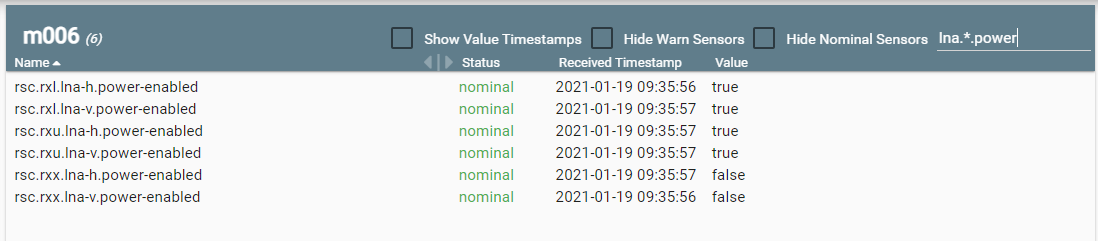
\includegraphics[scale=0.4]{Chapters/images/image41.png}
	
	%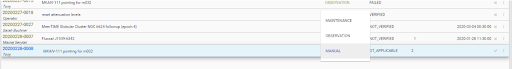
\includegraphics[resolution=100]{bur1.png}
	\caption{Sensor list showing LNA status}
	\label{fig:image41}
\end{figure} 
\section{ 2nd Stage Amplifiers}

To switch them on if they are off, again in the ipython session do the following:

\begin{lstlisting}[style=DOS]
cam.m0xx.req.rsc_rx(l)_amp2_h_power('enable')
cam.m0xx.req.rsc_rx(l)_amp2_v_power('enable')
\end{lstlisting}

To check if they are on, select\\
\sensor{Main menu} $>$ \sensor{Sensor List}  $>$ \sensor{m0XX} $>$ \sensor{rsc.rxl.amp2$-$h.power$-$enabled nominal true}

The image in \textbf{Figure}~\ref{fig:image51} shows that and stage amplifiers for \component{m006}, L, UHF and S-band receivers are switched on, i.e. enabled.

\begin{figure}[!thb]
	\centering
	
	%\includegraphicsdpi{100}{}{bur1.png}     
	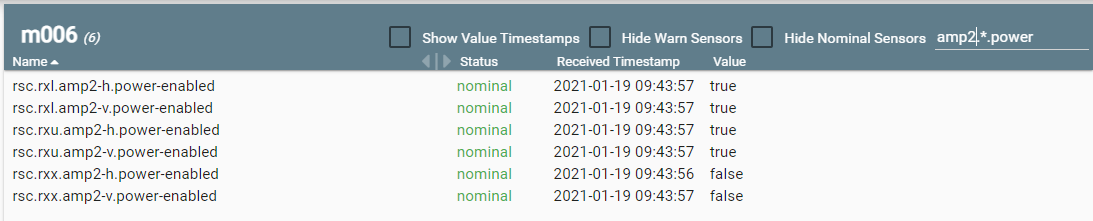
\includegraphics[scale=0.4]{Chapters/images/image51.png}
	
	%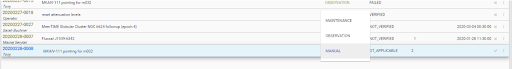
\includegraphics[resolution=100]{bur1.png}
	\caption{Sensor list showing stage 2 amplifiers}
	\label{fig:image51}
\end{figure} 

\section{ Helium Compressor}
The helium compressor supplies high pressure helium to the cryocoolers of the respective receivers. This means one helium compressor is connected to all working receivers on an AP. 

Hence if a fault occurs on the helium compressor, it will shut down causing all receivers (L-band, UHF-band and S-band) on the AP to warm up, making AP unusable for observations. There are usually two types of Helium compressor faults that occur:
\subsection{ Helium compressor pressure fault}
\textbf{Figure}~\ref{fig:He1} shows the sensors that go into error when a pressure fault occurs.

\begin{figure}[!thb]
	\centering
	%\includegraphicsdpi{100}{}{bur1.png}     
	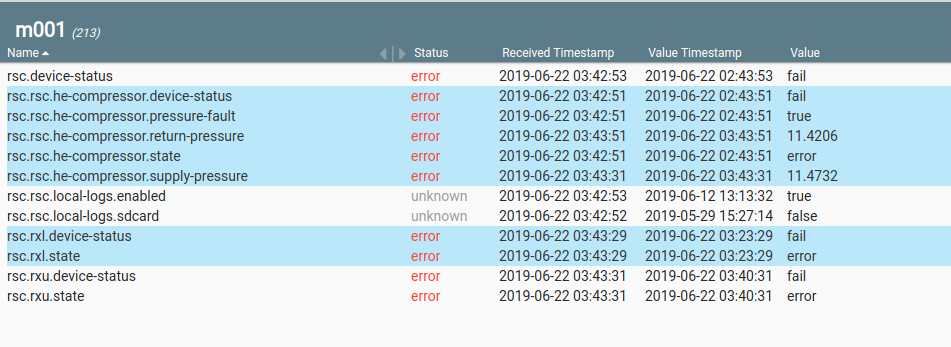
\includegraphics[scale=0.45]{Chapters/images/He1.png}
	
	%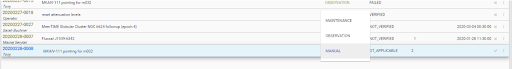
\includegraphics[resolution=100]{bur1.png}
	\caption{Receiver System Hellium presure errors}
	\label{fig:He1}
\end{figure}
\subsection{Helium compressor temperature fault}
\textbf{Figure}~\ref{fig:He2} shows the sensors that go into error when a temperature fault occurs.
Note the only difference in sensors between the two faults mentioned above is the sensor indicating the type of fault:
rsc.rsc.he-compressor-pressure-fault (for pressure faults)
rsc.rsc.he-compressor-temp-fault (for temperature faults)

If one of these faults thus occur, report the issue as such (you don’t have to also report that the receivers are warm in a separate report, since helium compressor faults automatically cause receivers to warm up).

\clearpage
\begin{figure}[!thb]
	\centering
	%\includegraphicsdpi{100}{}{bur1.png}     
	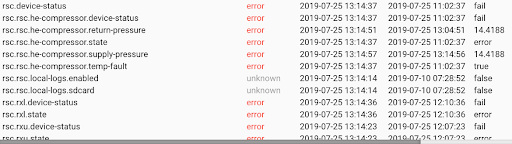
\includegraphics[scale=0.8]{Chapters/images/He2.png}
	
	%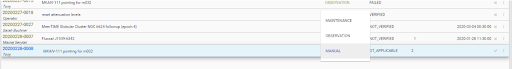
\includegraphics[resolution=100]{bur1.png}
	\caption{Receiver System temperature errors}
	\label{fig:He2}
\end{figure}



The following helium compressor sensors can be ignored (no action needed) when they go into error as they have no control value over the receivers and thus won’t affect observations in any manner:
\begin{itemize}
	\item{} \sensor{rsc.rsc.he-compressor.temperature1}
	\item{} \sensor{rsc.rsc.he-compressor.temperature2}
\end{itemize}

\section{ Receivers system debugging tools}
We have debugging tools for the receivers systems which technicians use to predict failures and reporting of the receiver system status.  (You can either choose the\file{rx\_daily} folder to view the daily receiver reports or the\file{rx\_monthly} folder to view the monthly receiver reports). The tool is written in an\package{IPYTHON} notebook and it is executed daily to provide daily reports. 

The following sensors can be ignored (no action needed as they are disabled and thus will show “unknown” status) as they have no control value over the receivers and thus won’t affect observations in any manner:
\begin{itemize}
	\item{} \sensor{rsc.rsc.local-logs.enabled}
	\item{} \sensor{rsc.rsc.local-logs.sdcard}
\end{itemize}

\begin{table}[h]
	
\caption{Receiver health by color coding.}
\label{tab:table1}

	\begin{tabular}[b]{|p{0.1cm}|p{0.6cm}|p{0.9cm}|p{0.2cm}|p{1.1cm}|p{1cm}|p{0.7cm}|p{0.2cm}|p{0.2cm}|p{1.1cm}|p{1.1cm}|p{1.1cm}|p{1.1cm}|}
		\hline
		
	\multicolumn{7}{|c|} {\done Green: Ok}& & & & &\\
		\hline
		\multicolumn{7}{|c|} {\hcya Yellow : System usable but report maintenance for schedule correction}& & & & &\\
		\hline	
		\multicolumn{7}{|c|} {\hcy Orange : System usable but monitor and report to maintanace if stte persist}& & & & &\\
		\hline
		\multicolumn{7}{|c|} {\hcyan Red : Do not use and report to maitenance immidiately}& & & & &\\
		\hline	
		\multicolumn{7}{|c|} {\hc Blue: Operator can change state}& & & & &\\
		\hline			
			& & & & & & & & & & &\\
		\hline
			 &m007 &Receiver System & 32& rsc& 14&rsc.current & 1& &  & &\\
		\hline
			& 1& Window&1 & & & rsc.voltage &1& & & &\\
		\hline
			& & & & & & & & & & &\\
		\hline
			& & & & & & & & & & &\\
		\hline
			& & & & & & & & & & &\\
		\hline
			& & & & & & & & & & &\\
		\hline
			& & & & & & & & & & &\\
		\hline
			& & & & & & & & & & &\\
		\hline
			& & & & & & & & & & &\\
		\hline
			& & & & & & & & & & &\\
		\hline
			& & & & & & & & & & &\\
		\hline
			& & & & & & & & & & &\\
		\hline
			& & & & & & & & & & &\\
		\hline
			& & & & & & & & & & &\\
		\hline
			& & & & & & & & & & &\\
		\hline
	\end{tabular}


\end{table}






 
 \chapter{ AP Subsystem}
 
 \section{Motion Profilers}

A profiler is needed because the servo loops are high gain loops; large position steps in 
a high gain system would inevitably lead to large overshoots. The profiler smoothens both the velocity and the acceleration profile. It ensures that the position controller is fed with small position increments only. It also provides velocity and acceleration feed forwards. The acceleration feed forward is enabled only in case of transitions between trajectories. Profiler handling is done automatically by the ACU. External commands from ACU or CAM may include any size of position steps within the operating range.

\subsection{ To check if profilers are on or off}
It is required that profiles are always enabled on the AP at all times. But it is advisable that operators check the status of the profilers form time to time. 
\begin{lstlisting}[style=DOS]
ssh kat@obs.mkat.karoo.kat.ac.za
Ipython
Import katuilib
configure_cam('camcam', 'all')
cam.print_sensors('profiler')
\end{lstlisting}





\subsection{ To switch profilers off}
\begin{lstlisting}[style=DOS]
cam.m0XX.req.ap_enable_motion_profiler('elev', 0)
cam.m0XX.req.ap_enable_motion_profiler('azim', 0)
\end{lstlisting}




\subsection{To switch profilers on}
\begin{lstlisting}[style=DOS]
cam.m0XX.req.ap_enable_motion_profiler('elev', 1)
cam.m0XX.req.ap_enable_motion_profiler('azim', 1)

\end{lstlisting}


\section{ AP Point Error Tiltmeters}
The tiltmeter measures the the tilt of the antenna tower and by using a tiltmeter, pointing errors due to non-orthogonality of the azimuth axis and deformations of the azimuth structure because of temperature and constant wind can be compensated to a large extent [TBD]. The tiltmeter shall always be enabled.  The status of the tiltmeter can be checked from the ipython session. In the obs  machine do the following:
\begin{lstlisting}[style=DOS]
ipython
import katuilib
configure_cam('camcam',all)
\end{lstlisting}


\subsection{To check the status of the point error tiltmeter sensor}
\begin{lstlisting}[style=DOS]
cam.print_sensors('point_error_tiltmeter')
\end{lstlisting}


\subsection{To enable the tiltmeter sensor}
\begin{lstlisting}[style=DOS]
cam.m00X.req.ap_enable_point_error_tiltmeter(1)
\end{lstlisting}



The output will be as follows
\begin{lstlisting}[style=DOS]
!ap-enable-point-error-tiltmeter ok
\end{lstlisting}



\subsection{ To enable all antennas}
\begin{lstlisting}[style=DOS]
cam.ants.req.ap_enable_point_error_tiltmeter(1)
\end{lstlisting}



\subsection{To disable the tiltmeter sensor}
\begin{lstlisting}[style=DOS]
cam.m00X.req.ap_enable_point_error_tiltmeter(0)
\end{lstlisting}



The output will be as follows
\begin{lstlisting}[style=DOS]
!ap-enable-point-error-tiltmeter ok
\end{lstlisting}


 
\section{ Test observations scripts} 
\subsection{SE tilt sensor measurements observations} 
The purpose of the tilt measurements is to look at calibration tilt sensors and also to calculate tilt sensor offset parameters and compare these with set values. From a single test the calculated tilt sensor parameters did not match that closely to the set values. We were hoping to take many measurements so that we could see from the average of a number of low wind measurements if the calculated value matched the set values, especially for receptors where the calibration had recently been checked.   The next step was going to be to get to a point whereby we could automatically write the calculated values to the ACU to update the values. We have not reached that point yet.


\subsection{ Ap.rate\_test.py}

This script rotates the AP at elevation 20 tilt measurements. This script is no longer used and was applicable during acceptance testing and commissioning.
\subsubsection{ Ap.rate\_test.py fails due to timeout}
\begin{itemize}
	\item[] \textbf{cause}: the timeout happens because some of the antennas become unresponsive during the measurement.
	\item[] \textbf{consequences}:  currently this causes the script to terminate with a messy error message $-$ fortunately it doesn’t mess up the telescope state (as it used to do earlier in the year). when this happens the first 1/2 of the script gets completed correctly, just the second 1/2 is interrupted. The second 1/2 is essentially a repeat of the first, so there’s still useful data here.
	\item[] \textbf{recommendations}: the current behaviour is messy but not intolerable.  the script should be made more robust against this, to continue with the remaining antennas.
		
\end{itemize}






\subsection{Reporting AP Struct Tilt x/y  in error}
Risk
\begin{itemize}

\item{} Pointing offsets
\end{itemize}
Procedure 
\begin{itemize}
\item{} Inspect the status of tilt sensors in the GUI sensor list  
\begin{itemize}

	\item[] ap.struct$-$tilt$-$x  	\textcolor{red} {error}  	$2019-07-12 \quad 14:59:06$
	\item[] ap.struct$-$tilt$-$y  	\textcolor{red} {error} $2019-07-12 \quad 14:59:16-190.64$
\end{itemize}



When reporting this error include the following in the JIRA to determine the course and action.
\begin{itemize}
	\item[$\circ$] Check the  ap temp $-$ plot sensorgraph
	\item[$\circ$] Check ap motion $-$ plot azim and elev actual sensors
	\item[$\circ$] Is $x/y$ tilt getting larger(correction value)? (Plot struct tilt $x/y$ on sensorgraph)
	\item[$\circ$] Or is it a sudden jump to error? 
	\item[$\circ$] Checking these trends below will answer the question as to whether this is a matter of calibrating with correct values or is it a structural problem or not.
	
	
	
	
\end{itemize}
\item{} Report the JIRA to site AP teachnicians
\end{itemize}
 
 \chapter{Engineering and Maintenance}
 Every Wednesday is reserved for maintenance, upgraded and deployment of new software and hardware. This time is usually given to engineers and technicians to sort out issues and faults that have been reported by Telescope Operators in Userlogs and Jiras.  There are still observations that are carried out depending on the number of antennas. But this day is mainly used for integration testing and bug fixing. 
\section{ Flights}
On Wednesday morning, a flight takes off from Cape Town International Airport with a number of engineers who go to site to do different types of tasks like hardware installation, testing, bug fixes etc on site. For days and times when there will be a flight arriving on site, it is important to stow the receptors away from the flight path. The flight company usually sends the ETA for the destination at Losberg and the flight arrival and departures are marked on the site calendar. The procedure to follow is to build a subarray and then use the  following schedule block (SB), which must be verified on the GUI and run as an observation, ensure that receptors are pointing all at elevation 18 deg.\\
In ipython session do the following commands:

\begin{lstlisting}[style=DOS]
configure_obs()
obs.sb.new(owner="Operator") 
obs.sb.type = katuilib.ScheduleBlockTypes.OBSERVATION
obs.sb.description = "Lower APs for Flight arrival and departure" 
obs.sb.instruction_set= "run-obs-script /home/kat/katsdpscripts/utility/flight_stow.py"
obs.sb.to_defined()
obs.sb.to_approved()
obs.sb.unload()
\end{lstlisting}

You can run the observation like any other observation except there is no need to include other resources like cbf and sdp in the subarray. 

\section{ ComRAD}

Use this tool to track Execujet flights every Wednesday so to stow/unstow antennas to protect the receivers\cite{ComRAD}.
\url{http://comradgis.kat.ac.za:8000/login}\\
You can create your own username and password. 

\chapter{Telescope Control Procedure}
 

\section{The Site Calendar}
The site calendar is used to schedule all observations and testing that is carried out on meerKAT telescope. The operator will typically follow the instructions that are scheduled on this calendar to do global sync, calibration, stowing the antennas for flights, build subarrays etc. The operator will be required to do the following as per the calendar entries:

\begin{itemize}	
\item{}	Verify that you are on AR1\_site calendar, see \textbf{Figure}~\ref{fig:calendar} below for depiction of the site calendar.

\item{} If no schedule block (SB) is assigned, then proceed to the section below.
	
	
\end{itemize}




\begin{figure}[!thb]
	\centering
	%\includegraphicsdpi{100}{}{bur1.png}     
	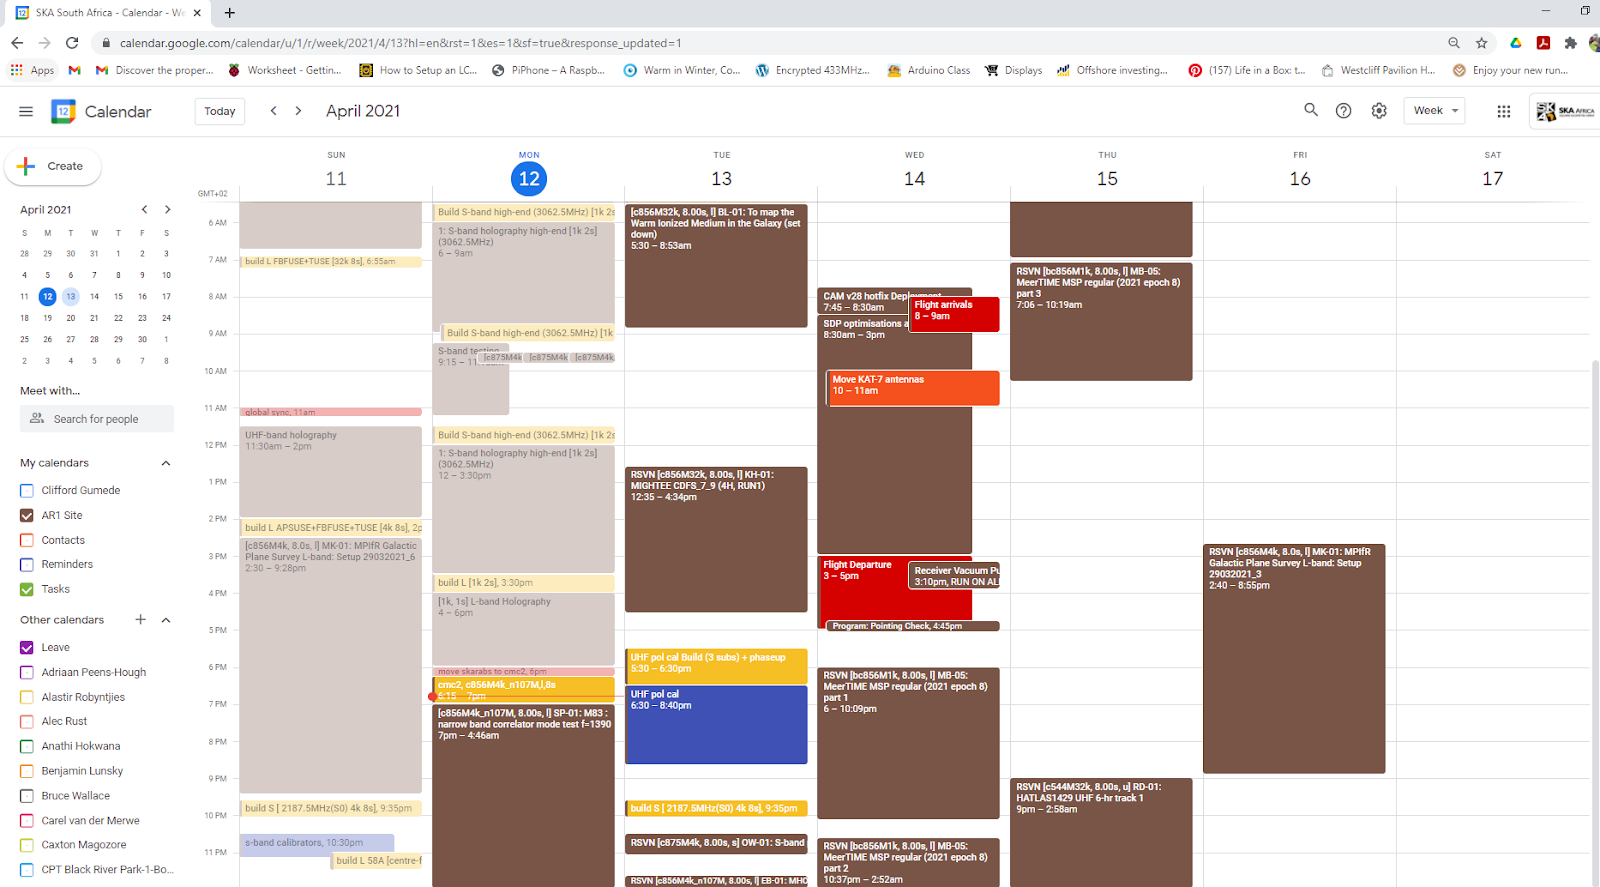
\includegraphics[scale=0.25]{Chapters/images/calendar.png}
	
	%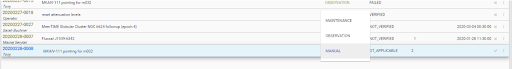
\includegraphics[resolution=100]{bur1.png}
	\caption{Google calendar for site activities}
	\label{fig:calendar}
\end{figure}
\section{ Create a New Schedule Block (SB)}
Connect to obs machine via 
\begin{lstlisting}[style=DOS]
ssh kat@obs.mkat.karoo.ac.za
ipython
Import katuilib
configure_obs()
\end{lstlisting}

	
Paste the schedule block details as shown in the image below in \textbf{Figure}~\ref{fig:image3} and run from the calendar event (observation).


\begin{figure}[!thb]
	\centering
	%\includegraphicsdpi{100}{}{bur1.png}     
	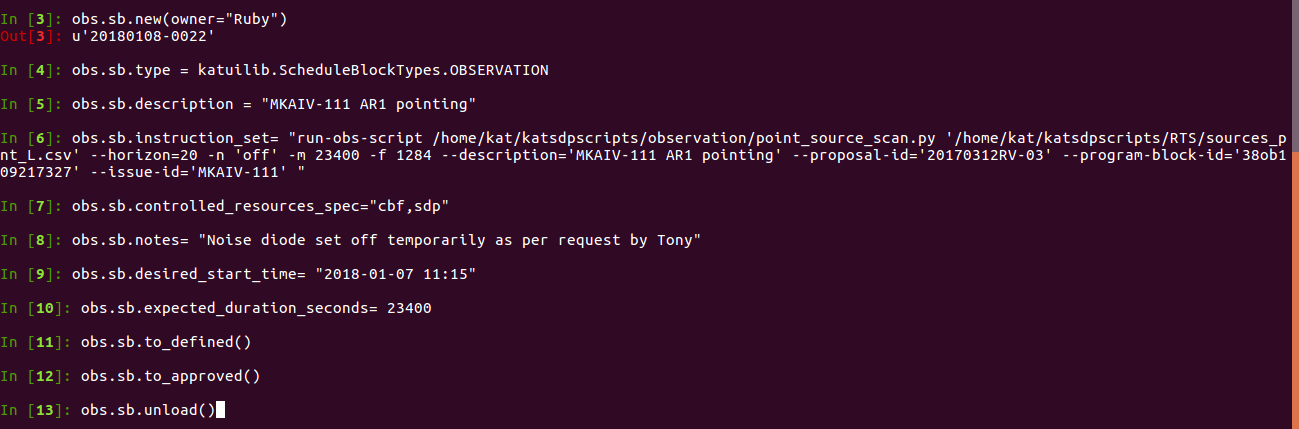
\includegraphics[scale=0.35]{Chapters/images/image3.png}
	
	%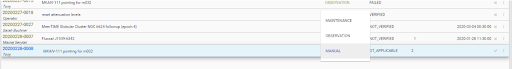
\includegraphics[resolution=100]{bur1.png}
	\caption{SB pasted on ipython sesion}
	\label{fig:image3}
\end{figure}
The commands above when ran in this ipython session will create a new SB in the GUI as shown in \textbf{Figure}~\ref{fig:image6}.

\begin{figure}[!thb]
	\centering
	%\includegraphicsdpi{100}{}{bur1.png}     
	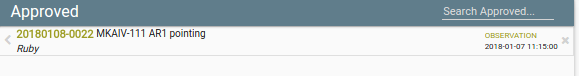
\includegraphics[scale=0.8]{Chapters/images/image6.png}
	
	%\includegraphics[resolution=100]{bur1.png}
	\caption{CAM GUI approved SB }
	\label{fig:image6}
\end{figure}

\section{Retrieve Old Schedule Blocks}
If you need to find a schedule block (SB) that is no longer found in the complete SB history in the GUI as shown in \textbf{Figure}~\ref{fig:image44} below. 

\begin{figure}[!thb]
	\centering
	%\includegraphicsdpi{100}{}{bur1.png}     
	\includegraphics[scale=0.35]{Chapters/images/image44.png}
	
	%\includegraphics[resolution=100]{bur1.png}
	\caption{Completed SB search}
	\label{fig:image44}
\end{figure}

Connect to the obs machin by ssh and run the commands as shown in \textbf{Figure}~\ref{fig:image116} .
\begin{lstlisting}[style=DOS]
ssh kat@obs.mkat.karoo.kat.ac.za
\end{lstlisting}



\begin{figure}[!thb]
	\centering
	%\includegraphicsdpi{100}{}{bur1.png}     
	\includegraphics[scale=0.35]{Chapters/images/image116.png}
	
	%\includegraphics[resolution=100]{bur1.png}
	\caption{SB search in the obs machine}
	\label{fig:image116}
\end{figure}
Select the schedule block number that you need.
You can view the contents of the schedule block by running the following commands on the ipython session: 

\begin{lstlisting}[style=DOS]
configure_obs()
obs.sb.new_clone(sb_number'
obs.sb.load('new_sb_number' )
\end{lstlisting}


If you do not know what the SB number is but know when the observation ran, run the following commands to display list of activities as shown in \textbf{Figure}~\ref{fig:image42}
\begin{lstlisting}[style=DOS]
ssh kat@portal.mkat.karoo.kat.ac.za
cd /var/kat/log$ 
less activity.2020-05-27.log  (you can choose the date of the log you want to view)
\end{lstlisting} 



\begin{figure}[!thb]
	\centering
	%\includegraphicsdpi{100}{}{bur1.png}     
	\includegraphics[scale=0.25]{Chapters/images/image42.png}
	
	%\includegraphics[resolution=100]{bur1.png}
	\caption{Open SB log file}
	\label{fig:image42}
\end{figure}
Zoom in on the screenshot to see schedule block numbers that ran/dry-ran on your chosen date.

\section{ Build a subarray (SA) suitable for the SB (observation)}
Select and load the desired resources from the free resources. These are:
Receptors (AP)
The correlator (\component{cbf\_x}) for \server{cmc1} or \component{cbf\_dev\_x} for \server{cmc2}
Science Processor (\component{sdp\_x})
Note that the Correlator and Science Processor proxy numbers denoted by \component{\_x} must match the subarray number (1 to 4) 
Select the data user product (List provided in drop down menu) 
Select desired frequency band (l,u,s or x)
Select desired dump rate (list provided in drop down menu)
If the dump rate was not specified for the SB (observation) leave the default setting as is.
Select APSUSE, FBFUSE, PTUSE and TUSE and if neededActivate the subarray. When the array is active, it will appear green in \textbf{Figure}~\ref{fig:image113}
\begin{figure}[!thb]
	\centering
	%\includegraphicsdpi{100}{}{bur1.png}     
	\includegraphics[scale=0.25]{Chapters/images/image113.png}
	
	%\includegraphics[resolution=100]{bur1.png}
	\caption{Active subarray with\component{cbf\_1} and \component{sdp\_1} resources}
	\label{fig:image113}
\end{figure}

Verify the SB by clicking on the far right dots of sb, see \textbf{Figure}~\ref{fig:image12}.


\begin{figure}[!thb]
	\centering
	%\includegraphicsdpi{100}{}{bur1.png}     
	\includegraphics[scale=0.25]{Chapters/images/image12.png}
	
	%\includegraphics[resolution=100]{bur1.png}
	\caption{ Verifying a SB }
	\label{fig:image12}
\end{figure}
\begin{itemize}
\item While verifying, check the dry run,
\item run the Schedule Block 
\item Schedule the SB
\item Execute the schedule
\item Scheduler modes should be in 
\begin{itemize}
\item[$\circ$] Manual - manual control over observation start-ups
\item[$\circ$] Queue - observations will automatically run as per queue
\end{itemize}
\end{itemize}
\section{ Alternative SA building using IPython session for debugging}

\#Creating a small subarray using python session
\begin{lstlisting}[style=DOS]
f=configure_subarray('test', 1)  ## build  a subarray (this is after the subarray is activated in the GUI), 'test' is the name of subarray '1' stand for subarray 1.
f.sub.sensor.number_ants.get_value()  ## to check if the subarray is active
f.ants.req.mode("STOP")
f.ants.req.target_azel(200,15)
f.ants.req.mode("POINT")
\end{lstlisting} 


This example illustrate how to run a subarray manually using CAM commands

\section{ Converting type of SB from 'MANUAL' to 'OBSERVATION'}

There are times when instruction sets could generate schedule blocks on the GUI with the observation type as MANUAL as in  \textbf{Figure}~\ref{fig:image19} :


\begin{figure}[!thb]
	\centering
	%\includegraphicsdpi{100}{}{bur1.png}     
	\includegraphics[scale=0.25]{Chapters/images/image19.png}
	
	%\includegraphics[resolution=100]{bur1.png}
	\caption{Manual SB}
	\label{fig:image19}
\end{figure}

If this happens, the dry run and progress log will be empty. The observation type can be changed on the GUI by following the steps below:

First assign the SB to the subarray as shown in  \textbf{Figure}~\ref{fig:image131}


\begin{figure}[!thb]
	\centering
	%\includegraphicsdpi{100}{}{bur1.png}     
	\includegraphics[scale=0.25]{Chapters/images/image131.png}
	
	%\includegraphics[resolution=100]{bur1.png}
	\caption{A SB assigned  to a subarray\_2}
	\label{fig:image131}
\end{figure}

Click on ‘SB APPROVED’, see  \textbf{Figure}~\ref{fig:image119}


\begin{figure}[!thb]
	\centering
	%\includegraphicsdpi{100}{}{bur1.png}     
	\includegraphics[scale=0.25]{Chapters/images/image119.png}
	 
	%\includegraphics[resolution=100]{bur1.png}
	\caption{Approved SB}
	\label{fig:image119}
\end{figure}

Choose ‘Edit’ as shown in \textbf{Figure}~\ref{fig:image31}
\begin{figure}[H]
	\centering
	%\includegraphicsdpi{100}{}{bur1.png}     
	\includegraphics[scale=0.25]{Chapters/images/image31.png}
	
	%\includegraphics[resolution=100]{bur1.png}
	\caption{Edit the approved SB}
	\label{fig:image31}
\end{figure}


Choose ‘OBSERVATION’ in the drop-down menu under ‘TYPE’

\begin{figure}[H]
	\centering
	%\includegraphicsdpi{100}{}{bur1.png}     
	\includegraphics[scale=0.37]{Chapters/images/image53.png}
	
	%\includegraphics[resolution=100]{bur1.png}
	\caption{Save SB as observation type}
	\label{fig:image53}
\end{figure}


Save that option by clicking on the tick



\begin{figure}[!thb]
	\centering
	%\includegraphicsdpi{100}{}{bur1.png}     
	\includegraphics[scale=0.4]{Chapters/images/ManualSB.png}
	
	%\includegraphics[resolution=100]{bur1.png}
	\caption{Save the edited SB }
	\label{fig:ManualSB}
\end{figure}

If you verify the SB this time, it should give you a dry run.

\section{Reset Attenuations}

This script can be run immediately after building an array when antennas have been out for maintenance or when changing between bands.

The power level into the digitiser (\sensor{rfcu.hpol.rf.power.in}) cannot be adjusted as this is a measure of the signal power produced by the receiver. Gain adjustment inside the receiver is not possible. If this power level is in error, operations should investigate the health of the receiver.
Operations can, and should, however adjust the power level that enters the ADC (\sensor{adc.hpol.rf.power.in}). If this sensor is in ERROR, operations should firstly verify the state of the RF power into the digitiser (\sensor{rfcu.hpol.rf.power.in}) to ensure that it is not in ERROR. If not the gain of the digitiser should be determined to ensure that it is within limits. Once it has been verified that the gain is within limits, the digitiser attenuation must be decreased until the power level into the ADC is within limits. There is no need for all the attenuators to be set to the same value. The reason for the attenuators is to adjust each receptor values individually. I therefore expect to see variations in attenuation across the array.

The second thing to remember is that the digitiser has a lot of dynamic range which means that there is very little chance of any saturation happening in the digitiser. You should therefore not unnecessarily add attenuation. It would be better to reduce attenuation (more gain) than add attenuation.

Attenuation levels should always be set to appropriate levels depending on the target brightness.  For very bright sources, attenuation levels are set at 31.  For most of our observations attenuation levels are set 6 for L-band.

Source:
\begin{lstlisting}[style=DOS]
kat@obs.mkat.karoo.kat.ac.za:~$ less STANDARD_SCHEDULE_BLOCKS.TXT 
\end{lstlisting}


In the obs machine, you must login ipython session and run: 
\begin{lstlisting}[style=DOS]
configure_obs()
obs.sb.new(owner='SeanPassmoor')
obs.sb.type=katuilib.ScheduleBlockTypes.OBSERVATION
obs.sb.description='Reset  attenuation levels'
obs.sb.antenna_spec='available'
obs.sb.instruction_set="run-obs-script /home/kat/katsdpscripts/utility/set_attenuation.py /home/kat/katsdpscripts/utility/AttenuationValues.csv"
obs.sb.to_defined()
obs.sb.to_approved()
\end{lstlisting}



You may consult with the AOD if the power levels do not look levelled, or look suspicious. There is a script below that you can run to refine attenuations found in the same folder above.

On the terminal, run:
\begin{lstlisting}[style=DOS]
ssh kat@obs.mkat.karoo.kat.ac.za
ipython
\end{lstlisting}
and paste the following SB:

\begin{lstlisting}[style=DOS]
configure_obs()
obs.sb.new(owner="SeanPassmoor") 
obs.sb.type = katuilib.ScheduleBlockTypes.OBSERVATION
obs.sb.description = "Refine Attenuation" 
obs.sb.antenna_spec="available"
obs.sb.instruction_set= "run-obs-script /home/kat/katsdpscripts/utility/refine_attenuation.py"
obs.sb.proposal_id='CAL-Attenuate'
obs.sb.to_defined()
obs.sb.to_approved()
obs.sb.unload()

\end{lstlisting}

\section{ Setting digitiser attenuation via ipython session}
On the \server{obs} machine/server. Configure a cam object:
 \begin{lstlisting}[style=DOS]
 ssh kat@obs.mkat.karoo.kat.ac.za
 ipython
 import katuilib
 configure_cam('camcam','all')
 \end{lstlisting}


Check attenuation:
\begin{lstlisting}[style=DOS]
cam.print_sensors('attenuation')

\end{lstlisting}

The steps below must be done before building a subarray but it is not advisable to set attenuations manually as there is a script that  was developed that has automated this process. These steps below can be used for test purposes only.


\subsection{ To attenuate all digitiser}
\begin{lstlisting}[style=DOS]
cam.ants.req.dig_attenuation('h',6)  
cam.ants.req.dig_attenuation('v',6)
\end{lstlisting}

This will apply attenuation of 6 to both vertical (v) and horizontal(h) polarisations of all antennas. This must not be done under any circumstances unless debugging the system. 
\subsection {To attenuate a single digitiser}
\begin{lstlisting}[style=DOS]
cam.m0xx.req.dig_attenuation('h',6)  
cam.m0xx.req.dig_attenuation('v',6) 
\end{lstlisting}
 
\section{ Delay Calibration and Phase-ups}
This is done to ensure that the signal has a phase difference of zero. Solutions close to zero are acceptable but monitor the waterfall plot as indicated below if unsure. To find a procedure on how access signal displays and plot waterfall displays go, go to the section called “Monitor an active observation” in this manual.

Risk
Incorrect delay solutions or out of phase signal data on some baselines

Source:
\begin{lstlisting}[style=DOS]
kat@obs.mkat.karoo.kat.ac.za:~$ less STANDARD_SCHEDULE_BLOCKS.TXT
\end{lstlisting}

 

\file{calibrate\_delays} and \file{bf\_phaseup} have been updated to use the new 'default' gain feature in CBF. It is no longer necessary to specify \option{fft-shift} and \option{f-engine-gain} options in the instruction set. 
Run a delay cal immediately after every new subarray build
Monitor the progress output of the script and waterfall plot of all baselines

\subsection{Delay calibration SB}
The following SB is the Standard delay calibration. This can be run for 1K, 4K, 32K and in UHF-band and L-band.
\begin{lstlisting}[style=DOS]
configure_obs()
obs.sb.new(owner='Operator')
obs.sb.type=katuilib.ScheduleBlockTypes.OBSERVATION
obs.sb.controlled_resources_spec='cbf,sdp'
obs.sb.description='Delaycal'
obs.sb.instruction_set="run-obs-script /home/kat/katsdpscripts/observation/calibrate_delays.py '/home/kat/katsdpcatalogues/three_calib.csv' -t 128"
obs.sb.proposal_id='CAL-20200106-OP-02'
obs.sb.notes='Delay calibration.'
obs.sb.to_defined()
obs.sb.to_approved()
obs.sb.unload()
\end{lstlisting}


\subsection {Phaseup calibration SB}
The following SB is the Standard phase up with bandpass flattening. This can be run for 1K, 4K, 32K and in UHF-band and L-band.
\begin{lstlisting}[style=DOS]
configure_obs()
obs.sb.new(owner='Operator')
obs.sb.type=katuilib.ScheduleBlockTypes.OBSERVATION
obs.sb.controlled_resources_spec='cbf,sdp'
obs.sb.description='Phase up with flatten bandpass'
obs.sb.instruction_set="run-obs-script /home/kat/katsdpscripts/observation/bf_phaseup.py '/home/kat/katsdpcatalogues/three_calib.csv' -t 256 --flatten-bandpass"
obs.sb.proposal_id='CAL-20200106-OP-03'
obs.sb.notes='Phase up with bandpass flattening.'
obs.sb.to_defined()
obs.sb.to_approved()
obs.sb.unload()
\end{lstlisting}

 
\textbf{Accepted waterfall plots} - in  \textbf{Figure}~\ref{fig:image1}, looking from the top of each y-axis baseline block (time)
Green colour means there is no phase difference - this is good. Other colours are acceptable too. These are minor differences.


\begin{figure}[!thb]
	\centering
	%\includegraphicsdpi{100}{}{bur1.png}     
	\includegraphics[scale=0.37]{Chapters/images/image1.png}
	
	%\includegraphics[resolution=100]{bur1.png}
	\caption{Acceptable waterfall plot}
	\label{fig:image1}
\end{figure}

\begin{itemize}
	\item {} For \textbf{all observation types},  noisy output/incoherent signal output is not acceptable, mark that antenna faulty.
	

	\item {} For \textbf{imaging observations}, phase wrapping can be corrected by the Astronomer, do not mark that antenna faulty.
	\item {} For \textbf{Holography and Pulsar observations}, any large delay solution values, mark the antenna faulty.
	
\end{itemize}




\subsection{  Delay Cal Script Fails:}

Delay solutions not found:\\
\option{\textcolor{red}{
2020-08-31 16:32:39.386Z WARNING   - m063h:      0.000 ns, delay fit failed (all its data probably flagged)\\
2020-08-31 16:32:39.387Z WARNING   - m063v:      0.000 ns, delay fit failed (all its data probably flagged)}
}\\

\begin{itemize}
\item{} Check \server{kat@portal.mkat.karoo.kat.ac.za:/var/kat/log}\$
(specific antenna log) - to see if the antenna misbehaved during the delay cal. e.g ap failures/proxy not in STOP when it should be.

\item{} Or check \server{kat@portal.mkat.karoo.kat.ac.za:/var/kat/log}\$ for\file{kat.cbfmon\_1} logs to see around that time that the array was built if there were any HMC or sync errors or any other cbf error regarding a F-host/X-host connected to that failed antenna.
\item{} Check cal pipeline logs via mesos in the GUI  

	
\end{itemize}

 

\section{ What could go wrong?}
\subsection{ Failed to select band while building array}
\begin{itemize}
\item{} One or more receptors failed to select observing band. The following error can be seen when building an array from the subarray logs:\\ \option{ 'select\_band\#012 raise faults. SelectBandError(failed)\#012SelectBandError: Failed to select\_band on receptors [m0xx]'} 
\item{} Wait for the building process to end, then press the retry button on the GUI.
\item{} If the above step fails, check the \sensor{'indexer raw position'} sensor in sensor list (see \textbf{Figure}~\ref{fig:image72}) for that receptor (e.g L band $=$ 40\unit{deg})

\begin{figure}[!thb]
	\centering
	%\includegraphicsdpi{100}{}{bur1.png}     
	\includegraphics[scale=0.37]{Chapters/images/image72.png}
	
	%\includegraphics[resolution=100]{bur1.png}
	\caption{CAM GUI sensor list to check indexer position}
	\label{fig:image72}
\end{figure}

If not on band, ssh into the obs machine as previously done.
\begin{lstlisting}[style=DOS]
ipython
import katuilib
configure_cam('camcam', 'all')
cam.m0xx.req.mode('STOP')
cam.m0xx.req.select_band('l', timeout=60) or 'u' for UHF  
cam.m0xx.req.ap_set_indexer_position('l') or 'u' for UHF
\end{lstlisting}


\item{} If the above step fails, check if the digitiser for the band in use is marked ready as shown in \textbf{Figure}~\ref{fig:image9}. If not refer to ‘mark digitiser ready’ section on this document, or follow the steps on the  Mark Digitiser Absent and/or Ready procedure.

\begin{figure}[!thb]
	\centering
	%\includegraphicsdpi{100}{}{bur1.png}     
	\includegraphics[scale=0.37]{Chapters/images/image9.png}
	
	%\includegraphics[resolution=100]{bur1.png}
	\caption{CAM GUI sensor list to check digitiser marking}
	\label{fig:image9}
\end{figure}
\item{} If unresolved, check if the digitiser serial number is the right one. To do this refer to the ‘Updating config for a replaced digitiser’ section on the document or follow the Checking digitiser serial numbers procedure. Should the wrong digitiser be marked ready or the issue remain unresolved contact CAM Support.
\end{itemize}

\subsection{ Multiple F-hosts in error after subarray build}

\begin{itemize}
	\item {}To identify the disabled f-hosts
	
	\begin{itemize}
		\item[$\circ$] Once the cbf is activated check the cbfmon plot in the GUI
		\item[$\circ$] The antennas appears as a green (zero) blocks in waterfall plot
		\item[$\circ$] You will see the signal for the affected antenna drop in the time series plot
		\item[$\circ$] You will also notice no ingest data on the signal display as shown in \textbf{Figure}~\ref{fig:image20}.   Type \option{flagcount} to display the figure below.
		
		
	\end{itemize}



 

\begin{figure}[!thb]
	\centering
	%\includegraphicsdpi{100}{}{bur1.png}     
	\includegraphics[scale=0.4]{Chapters/images/image20.png}
	
	%\includegraphics[resolution=100]{bur1.png}
	\caption{SDP flag count plot with one F-host disabled}
	\label{fig:image20}
\end{figure}

\item{} CBF should automatically disable a faulty F-HOST.
\item{} To verify cbf health, go to:\\ \url{http://cbf-nuc2.cpt.kat.ac.za/cmc1/array_1.wide}

\begin{figure}[!thb]
	\centering
	%\includegraphicsdpi{100}{}{bur1.png}     
	\includegraphics[scale=0.22]{Chapters/images/image40.png}
	
	%\includegraphics[resolution=100]{bur1.png}
	\caption{CBF health dashboard}
	\label{fig:image40}
\end{figure}

\item{} You can also check the sensors by looking at the CBFMON on the sensor list (hide nominal - this takes a while to load)
\item{} If multiple F-hosts are in error, break the array and build a new one [Remember to double check over a few minutes to see if the errors do not disappear by themselves.]
\item{} The other option is to check the health of CBF via the CAM GUI as shown in \textbf{Figure}~\ref{fig:image40} and \textbf{Figure}~\ref{fig:image91}

\end{itemize}


\begin{figure}[!thb]
	\centering
	%\includegraphicsdpi{100}{}{bur1.png}     
	\includegraphics[scale=0.26]{Chapters/images/image91.png}
	
	%\includegraphics[resolution=100]{bur1.png}
	\caption{CBF health pie charts}
	\label{fig:image91}
\end{figure}

\subsection{ Marking SKARAB Board on Standby}	
If these f-host errors are mapped to one particular bad skarab board call cbf to disable the board.
In obs machine type the following commands to check on CMC2:
\begin{lstlisting}[style=DOS]
kcpcmd -t 30 -s 10.103.254.3:7147 array-list
kcpcmd -t 30 -s 10.103.254.3:7147 resource-list|grep "up$" | wc -l 
kcpcmd -t 10 -s 10.103.254.3:7147 resource-mark skarab020408-01 standby 
\end{lstlisting}

\subsection{ No Descriptor Errors} 
\begin{itemize}
\item{} After a subarray is built run an observation to check that descriptors are being received.
\item{} It is a good idea to run a delay cal with a long “tail” \option{--verify-duration=300}, this will return to the source for 300s after the delays are found
\end{itemize}
\subsection{ Diagnostics}
\begin{itemize}
	\item{} When running the observation it is useful to have two signals displays (windows) open
	\begin{itemize}
		\item[$\circ$] Grafana
		  \item[$\circ$]    Go to the GUI, sensor list and select sdp\_1 , Monitor descriptors in sensor list (search 'desc')
		  \item[$\circ$] The no descriptor count should not be rising
		    
		  \item[$\circ$] There are four ingest nodes - each has 1/4 of the band   
		
	\end{itemize}
	


\item{} Example of “\textbf{no descriptor}” error
	\begin{itemize}
	\item[$\circ$] No descriptor block shows orange
\item[$\circ$] Part of the band is missing, see \textbf{Figure}~\ref{fig:image79} and \textbf{Figure}~\ref{fig:image65}.
\item[$\circ$] The no descriptor heap counts keeps rising as shown in \textbf{Figure}~\ref{fig:image37}
\end{itemize}
\end{itemize}



\begin{figure}[!thb]
	\centering
	%\includegraphicsdpi{100}{}{bur1.png}     
	\includegraphics[scale=0.2]{Chapters/images/image79.png}
	
	%\includegraphics[resolution=100]{bur1.png}
	\caption{SDP "no descriptors" error on Grafana}
	\label{fig:image79}
\end{figure}

\begin{figure}[H]
	\centering
	%\includegraphicsdpi{100}{}{bur1.png}     
	\includegraphics[scale=0.18]{Chapters/images/image65.png}
	
	%\includegraphics[resolution=100]{bur1.png}
	\caption{Part of band missing due to "no descriptors" error}
	\label{fig:image65}
\end{figure}

\begin{figure}[!thb]
	\centering
	%\includegraphicsdpi{100}{}{bur1.png}     
	\includegraphics[scale=0.25]{Chapters/images/image37.png}
	
	%\includegraphics[resolution=100]{bur1.png}
	\caption{SDP sensor list with no-descriptor count increasing}
	\label{fig:image37}
\end{figure}



\subsection{ How to fix this}
\begin{itemize}
	\item[\textbf{Step 1}] Stop the current observation.
	  \begin{itemize}
	    \item[$\circ$] Check the number of “no descriptor” errors, check x-host health, check leaf switches, and if they are okay continue to step 2.	
    \end{itemize}

\item[\textbf{Step 2}] Tear down the array for critical/urgent observations to continue.
 \begin{itemize}
 	\item[$\circ$] This should leave the failed subarray as a zombie within SDP for debugging, while continuing operations.
 	\item[$\circ$] To diagnose if this is an SDP problem: 
 	 \begin{itemize}
	\item[$\square$] Find the time at which the ingest process stopped working: this will show up as a sudden drop in the SDP input data rate. 
	\item[$\square$] Then check SDP’s (ingest) logs for a message like this at around the same time:
	 \begin{itemize}
	 \item{} \option{2019-10-27 15:59:58.558 ing4.sdp.mkat.karoo.kat.ac.za ingest.sdp\_l0.4: array\_1\_wide\_0  worker thread blocked by full ringbuffer on heap 8467887039}	
	   \end{itemize}
    \end{itemize}	
\end{itemize}
\item[\textbf{Step 3}] After following the above steps, rebuild the subarray and monitor the leaf switches health using the following command line on obs machine : 


\begin{lstlisting}[style=DOS]
ssh kat@obs.mkat.karoo.kat.ac.za

ssh kat@obs.mkat.karoo.kat.ac.za: ./usersnfs/cbf_support/display_switch_rates.py -d leaves
\end{lstlisting}









\end{itemize}

\subsection{CBF Data Capture Failed}
See the CBF data capture error the progress out put \\
\url{http://10.97.1.13:8081/tailtask/20180612-0012/progress}
\begin{itemize}
	\item{} This error on the cbf side is caused by a clash in resources (where some skarabs are being deprogrammed in the lower cbf levels by a non lead operator)
	\item{} Break the array
\begin{lstlisting}[style=DOS]
ssh telnet cmc1.cbf.mkat.karoo.kat.ac.za 7147
?resource-list (to see which resources are available)
\end{lstlisting}

	\item{} Try building again, if this error persists over several retries contact cbf to release resources
	\item{} There is no fix in place to stop interruptions such as these - look at JIRA below
\url{https://skaafrica.atlassian.net/browse/MKAIV-1169?filter=-2}



\end{itemize}
\subsection{SDP Capture Done Failure}


 Interim SOP for CAM subarray-product-ids that end up causing sdp proxy to go in error while running scripts or rebuilding subarray.
\begin{itemize}


 	\item{} Check via the observation script logs which is visible with a warning followed by an error message.

 
	\item{} Check via CAM sensor\-list for cam data proxy, sdp\_1; filter product$-$ids value. 
\url{http://portal.mkat.karoo.kat.ac.za/katgui/sensor-list?component=sdp\_1}

If it shows more than 2 values for that same subarray, then it's a clear indication to teardown and rebuild the subarray.

Example, on subarray\_1, you will see these values: \option{array\_1\_wide\_0, array\_1\_wide\_1}

\option{Subarray-product-ids  nominal  2019-11-28 13:52:20  array\_1\_wide\_0, array\_1\_wide\_1}

\item{} Tear-down and rebuild the same subarray.  This should clear the error
\item{} Re-check via CAM sensor-list for sdp\_1; use filter: subarray-product-ids, and it should show only one value as shown in \textbf{Figure}~\ref{fig:image43}.

\option{Subarray-product-ids  nominal  2019-11-28 13:52:20 array\_1\_wide\_0}

\begin{figure}[!thb]
	\centering
	%\includegraphicsdpi{100}{}{bur1.png}     
	\includegraphics[scale=0.7]{Chapters/images/image43.png}
	
	%\includegraphics[resolution=100]{bur1.png}
	\caption{Subarray product-ids}
	\label{fig:image43}
\end{figure}

\textcolor{red}{Note: Only use restarting the sdp proxies via CAM as a last resort or when instructed.}
\end{itemize}

\subsection{ Vaccs Lost Sync}
When vaccs lose sync an X-engine becomes disabled
\begin{itemize}

	\item{} If during an observation, data on some band suddenly disappears as shown in . Check the signal displays as shown \textbf{Figure}~\ref{fig:image24}
	\begin{figure}[!thb]
		\centering
		%\includegraphicsdpi{100}{}{bur1.png}     
		\includegraphics[scale=0.26]{Chapters/images/image24.png}
		
		%\includegraphics[resolution=100]{bur1.png}
		\caption{Data loss due to vaccs sync error}
		\label{fig:image24}
	\end{figure}

\item{} Run the check cbf health script in the obs machine
\begin{lstlisting}[style=DOS]
kat@obs.mkat.karoo.kat.ac.za:~$ ./katsdpscripts/utility/check_cbf_skarab.py  --strategy=detail
\end{lstlisting}

\item{} If the vaccs have lost sync, kill the array and build a new one
\item{} Write a JIRA with a sensorgraph as shown in \textbf{Figure}~\ref{fig:image27}



\begin{figure}[!thb]
	\centering
	%\includegraphicsdpi{100}{}{bur1.png}     
	\includegraphics[scale=0.26]{Chapters/images/image27.png}
	
	%\includegraphics[resolution=100]{bur1.png}
	\caption{CBF vaccs sync sensor graph}
	\label{fig:image27}
\end{figure}

\end{itemize}














\subsection{CBF Persistent mismatched sequence numbers}
\begin{itemize}

\item{} Apply procedure if only you are failing to build because of the errors shown in  \textbf{Figure}~\ref{fig:image95}:
\begin{figure}[!thb]
	\centering
	%\includegraphicsdpi{100}{}{bur1.png}     
	\includegraphics[scale=0.6]{Chapters/images/image95.png}
	
	%\includegraphics[resolution=100]{bur1.png}
	\caption{CBF mismatched sequence numbers error log}
	\label{fig:image95}
\end{figure}

\item{} When cbf only reports mismatched sequence errors, halt the array instrument on cmc1 and try again.  Get the array name first
\begin{lstlisting}[style=DOS]
kcpcmd -s cmc1.cbf.mkat.karoo.kat.ac.za:7147 array-list
\end{lstlisting}


\item{} Notice the highlighted instrument name in \textbf{Figure}~\ref{fig:image118} 


\begin{figure}[!thb]
	\centering
	%\includegraphicsdpi{100}{}{bur1.png}     
	\includegraphics[scale=0.6]{Chapters/images/image118.png}
	
	%\includegraphics[resolution=100]{bur1.png}
	\caption{CBF array name list}
	\label{fig:image118}
\end{figure}
\item{} Then halt the cbf instrument
\begin{lstlisting}[style=DOS]
kcpcmd -s cmc1.cbf.mkat.karoo.kat.ac.za:7147 array-halt array_name
\end{lstlisting}


\item{} Then rebuild the subarray. If you get the same error again alert the cbf team because they may need to replace the particular SKARAB board that is causing issues.
\end{itemize}


 \chapter{ MONITORING PROCEDURES}
 
\section{ Check CBF SKARAB Health}

Simply follow the link to see CBF overall health\\ \url{http://cbf-nuc2.cpt.kat.ac.za/cmc1/array\_1.wide} or \url{http://mon-cbf.kat.ac.za/}

\section{ MeerKAT Status Sensor Summary}
This too is a swift troubleshooting tool querying essential observation sensors from all active APs thus cutting down a systematic fault-finding approach.   

Log onto the obs mkat machine and run the script below and the output will appear  as shown in \textbf{Figure}~\ref{fig:image78} for L-band or \textbf{Figure}~\ref{fig:image107} for U-band:
\begin{lstlisting}[style=DOS]
ssh kat@obs.mkat.karoo.kat.ac.za
python usersnfs/tiyani/meerkat\_status.py --receiver-band rxl --send-status   

\end{lstlisting}


\begin{figure}[!thb]
	\centering
	%\includegraphicsdpi{100}{}{bur1.png}     
	\includegraphics[scale=0.18]{Chapters/images/image78.png}
	
	%\includegraphics[resolution=100]{bur1.png}
	\caption{Meerkat status script  output for U-band}
	\label{fig:image78}
\end{figure}



\begin{figure}[!thb]
	\centering
	%\includegraphicsdpi{100}{}{bur1.png}     
	\includegraphics[scale=0.23]{Chapters/images/image107.png}
	
	%\includegraphics[resolution=100]{bur1.png}
	\caption{Meerkat status script  output for L-band}
	\label{fig:image107}
\end{figure}

         




\section{ Monitor an active observation}
\subsection{Catalogues Not Matching The Observation}
If and when this happens, contact the AoD. Best practice to avoid it is by running a dryrun while there are still astronomers in the office

Once the observation begins,monitor the following for “no descriptor” errors:
\begin{itemize}

\item \textbf{no-descriptor}-heaps-total for each band on the sdp\_1 GUI sensor list. 
\item Go to the GUI, select sensor list and then select sdp\_1.
\item There are four ingest nodes where each has ¼ of the band.
\item Search for “desc” and hide nominals, the no-descriptor-heaps--total should preferably remain at zero for all ingest nodes (see \textbf{Figure}~\ref{fig:image129}) but there are times where one or two ingest nodes will increase for a very short period after the observation begins.

\begin{figure}[!thb]
	\centering
	%\includegraphicsdpi{100}{}{bur1.png}     
	\includegraphics[scale=0.26]{Chapters/images/image129.png}
	
	%\includegraphics[resolution=100]{bur1.png}
	\caption{SDP sensors}
	\label{fig:image129}
\end{figure}
\item This is okay, as long as they all do not keep increasing to very high numbers.If this happens then break down the subarray, reload the Mellanox switch and rebuild the array.
	




\item SDP Grafana GUI interface, this can be accessed via 	\url{http://mc1.sdp.mkat.karoo.kat.ac.za:3000/?orgId=1}  Select the "\textbf{Overview}" option. 

\item There are other options which are available from the dashboard as shown in \textbf{Figure}~\ref{fig:image11}.

\begin{figure}[H]
	\centering
	%\includegraphicsdpi{100}{}{bur1.png}     
	\includegraphics[scale=0.22]{Chapters/images/image11.png}
	
	%\includegraphics[resolution=100]{bur1.png}
	\caption{SDP Grafana dashboard}
	\label{fig:image11}
\end{figure}


When running the observation, the dashboard will most likely show “no descriptor” errors at the beginning of the observation.  No descriptor block and/or incomplete heaps block are orange, these values should return to zero within five minutes as shown in \textbf{Figure}~\ref{fig:image15}.

\begin{figure}[!thb]
	\centering
	%\includegraphicsdpi{100}{}{bur1.png}     
	\includegraphics[scale=0.22]{Chapters/images/image15.png}
	
	%\includegraphics[resolution=100]{bur1.png}
	\caption{SDP Grafana dashboard without \sensor{no descriptors} errors}
	\label{fig:image15}
\end{figure}
\end{itemize}
If the no descriptor counts keep rising, the switch needs to be reloaded

\begin{itemize}
\item Tail the observation progress,see  \textbf{Figure}~\ref{fig:image100}.


\begin{figure}[H]
	\centering
	%\includegraphicsdpi{100}{{bur1.png}     
	\includegraphics[scale=0.2]{Chapters/images/image100.png}
	
	%\includegraphics[resolution=100]{bur1.png}
	\caption{Observation progress log}
	\label{fig:image100}
\end{figure}


\item Load signal displays from  \url{ http://mc1.sdp.mkat.karoo.kat.ac.za:5004/}
You can also click on the link shown in \textbf{Figure}~\ref{fig:image126}, “Signal Display Dashboard ” under SDP resource.

\begin{figure}[H]
	\centering
	%\includegraphicsdpi{100}{}{bur1.png}     
	\includegraphics[scale=1]{Chapters/images/image126.png}
	
	%\includegraphics[resolution=100]{bur1.png}
	\caption{SDP signal display menu }
	\label{fig:image126}
\end{figure}

\item Type ‘load default2’ on the command line of the signal display \textbf{Figure}~\ref{fig:image50}.


\begin{figure}[H]
	\centering
	%\includegraphicsdpi{100}{}{bur1.png}     
	\includegraphics[scale=0.2]{Chapters/images/image50.png}
	
	%\includegraphics[resolution=100]{bur1.png}
	\caption{Default signal display}
	\label{fig:image50}
\end{figure}

If on the command line you type wtabhh  or wtabvv you will see displays similar to the one shown on Figure 53 and Figure 54 respectively. Here will be able to check for any faulty Receptors which are not phasing with other Receptors or may show noisy phase. 

\item{} Horizontal polarisations waterfall plot (wtabhh), this will display the waterfall in \textbf{Figure}~\ref{fig:image102}. polarisations. 
\clearpage

\begin{figure}[!thb]
	\centering
	%\includegraphicsdpi{100}{}{bur1.png}     
	\includegraphics[scale=0.23]{Chapters/images/image102.png}
	
	%\includegraphics[resolution=100]{bur1.png}
	\caption{Horizontal polarisation plot (wtabhh)}
	\label{fig:image102}
\end{figure}

\item{} Vertical polarisation waterfall plot (wtabvv), see \textbf{Figure}~\ref{fig:image36}



\begin{figure}[!thb]
	\centering
	%\includegraphicsdpi{100}{}{bur1.png}     
	\includegraphics[scale=0.23]{Chapters/images/image36.png}
	
	%\includegraphics[resolution=100]{bur1.png}
	\caption{Vertical polarisation plot (wtabvv)}
	\label{fig:image36}
\end{figure}

If for any reason, there is an antenna that is not phasing with other antennas or the phase seems noisy, then it is better to check if that antenna is moving with other antennas. You can open the receptor pointing tab and check the status of that antenna as shown in \textbf{Figure}~\ref{fig:image76} 


\begin{figure}[H]
	\centering
	%\includegraphicsdpi{100}{}{bur1.png}     
	\includegraphics[scale=0.2]{Chapters/images/image76.png}
	
	%\includegraphics[resolution=100]{bur1.png}
	\caption{Receptor pointing plot}
	\label{fig:image76}
\end{figure}


This will indicate to you if the antenna is locked on to the target by showing ‘*’ on the antenna number, if it is not locked to the target there will be no ‘*’. It will be advisable to look at the sensor list of that antenna in questions. 
There may be other reasons for an antenna to have a noisy phase like a warm receiver, LNA switched off or CBF errors. 

After the array is built  you can select “Sensor Groups” from the CAM GUI landing page and select critical observation sensors. This will list all the critical sensors that are required to be safe and okay for the observation as shown in \textbf{Figure}~\ref{fig:image125}.  

\end{itemize}

\begin{figure}[H]
	\centering
	%\includegraphicsdpi{100}{}{bur1.png}     
	\includegraphics[scale=0.2]{Chapters/images/image125.png}
	
	%\includegraphics[resolution=100]{bur1.png}
	\caption{CAM GUI List of critical sensors}
	\label{fig:image125}
\end{figure}


\section{ Monitoring SDP}

In order to see the status of the SDP subsystem after the array is built and the observation is running you can  start up the Science Processor dashboard (see \textbf{Figure}~\ref{fig:image123}). This dashboard called Grafana will give you all the information about the health of the SDP system and also data flow from CBF to SDP. 



\begin{figure}[H]
	\centering
	%\includegraphicsdpi{100}{}{bur1.png}     
	\includegraphics[scale=0.23]{Chapters/images/image123.png}
	
	%\includegraphics[resolution=100]{bur1.png}
	\caption{Grafana dashboard for SDP status}
	\label{fig:image123}
\end{figure}


There are more documents that have been written which describe procedures to be followed by operators when SDP encounters errors. 

\section{Monitoring Receptors}

Any faults on APs can be monitored by running the ipython session on obs.mkat.ka
\begin{lstlisting}[style=DOS]
ssh kat@obs.mkat.karoo.kat.ac.za

ipython

import katuilib
configure()

ant_inactive = sorted([ant.name for ant in kat.ants if ant.name \
in kat.katpool.sensor.resources_in_maintenance.get_value()])
ant_list = ''


for a in ant_inactive: ant_list = ant_list + a[2:] + '|'

ant_list = ant_list[:-1]

ap_sensors="(^m0(?!(%s|2(1|7).ap.ridx.hard.limit.*reached$)).*(connected|local.time|fail*|limit|(cb.*(sdc|pdc|digitiser1|receiver1|pump))|error|hatch|yoke|switch|ap.*mode|drive.power|read.error.count|rxl.(rfe1.temperature|lna.*.power.enabled)|(he.compressor.device)|windstow.active))|(dmc.*epoch)" % ant_list

kat.print_sensors(ap_sensors, strategy='period', status='warn|error|failure|unreachable')
\end{lstlisting}




This should generate the output as shown in \textbf{Figure}~\ref{fig:image124}.



\begin{figure}[H]
	\centering
	%\includegraphicsdpi{100}{}{bur1.png}     
	\includegraphics[scale=0.23]{Chapters/images/image124.png}
	
	%\includegraphics[resolution=100]{bur1.png}
	\caption{Output of antenna monitoring script}
	\label{fig:image124}
\end{figure}


\textbf{AP fault finding during observation:}
\begin{itemize}

\item  \textcolor{blue}{Exclude APs in Maintenance on Critical Observation Sensors}

Critical Observation Sensors is comprised of observation critical sensors. Sometimes receptors in maintenance flood the page when sensors transition to several non-nominal states, e.g. error, warn, failure, and unreachable. As this behavior is expected with maintenance, better to filter these receptors using regular expressions.  The example of how to do this is shown below in \textbf{Figure}~\ref{fig:image120}.

\item \textcolor{blue}{Filter out nominal sensors (default setting)}

Notice m024 sensors are mainly occupying the page as it is worked on. This could potentially mask a set of active APs in the process. Moreover, m017 and m018 digitizers are inactive, would you like to constantly monitor that? Of course not.



\begin{figure}[!thb]
	\centering
	%\includegraphicsdpi{100}{}{bur1.png}    1206.png}
	\includegraphics[scale=0.33]{Chapters/images/image120.png}
	%\includegraphics[resolution=100]{bur1.png}
	\caption{Critical observation sensors with hidden nominal sensors}
	\label{fig:image120}
\end{figure}

\item \textcolor{blue}{Excluding receptors}

For instance,\component{ m017, m018, m024, m025} and \component{m063} will be excluded. The expression is: m0(?!(17|18|24|25|63)) as shown in \textbf{Figure}~\ref{fig:image88}

\end{itemize}

\begin{figure}[!thb]
	\centering
	%\includegraphicsdpi{100}{}{bur1.png}     
	\includegraphics[scale=0.34]{Chapters/images/image88.png}
	
	%\includegraphics[resolution=100]{bur1.png}
	\caption{Critical sensor list filtered by AP names}
	\label{fig:image88}
\end{figure}


\section{ Monitoring CBF}
In order to monitor the status of the Correlator Beamformer (CBF) system, load the cbf mon\_1 plot on the GUI to monitor CBF health as shown in \textbf{Figure}~\ref{fig:image122}. 


\begin{figure}[H]
	\centering
	%\includegraphicsdpi{100}{}{bur1.png}     
	\includegraphics[scale=0.23]{Chapters/images/image122.png}
	
	%\includegraphics[resolution=100]{bur1.png}
	\caption{CBF monitor pie plots}
	\label{fig:image122}
\end{figure}

This will drill down to all the sensors of the CBF and will show warnings and alarms of each Skarab board. The dashboard will give you all the f-hots and x-hosts used in the array. Note that this display only becomes live after the subarray is built. 
It is important to know that for a normal wide band observation with 64 antennas, there will be 128 Skarabs used. 64 are used for F-engines and another 64 are used for X-engines.  But for wide band and narrow band, a total of 200 skarabs will be used for this observation. 

The alternative to looking at the CBF health status as shown in \textbf{Figure}~\ref{fig:image122} by using the following link:
\url{http://cbf-nuc2.cpt.kat.ac.za/cmc1/array\_1.wide}

If you want to see more CBF logs  you can monitor them by running cmc-top on the obs machine.
\begin{lstlisting}[style=DOS]
cmc-top cmc1.cbf.mkat.karoo.kat.ac.za:7147


\end{lstlisting}

\section{ Monitoring Digitiser }
\subsection{ Digitiser Spectrometer Overflows}

This is not a critical fail - it just reports that the power into the spectrometer causes the FFT to overflow (but it still works - much like an ADC saturation) - this is not supposed to happen, but it might be that the fft\_shift was decreased, causing this. 

This issue is that fft\_shift is set to 0 on a few digitisers (as opposed to 0xfffffffff) - this will cause FFT overflows. Must be at least 7. This is TBD at this stage.

\subsection{ Digitiser Deng Overflows}
When building a subarray, network problems (like the network interface crashing) can cause the digitiser to capture-start incorrectly, resulting in a deng overflow error. The f-host connected to this digitiser also a lot of times will give network reorder errors and thus appear red in the cbfmon1 plot. When you free the subarray, the error clears, but will appear again if you build a subarray again with the affected digitiser.

When this error occurs, the digitiser needs to be reconfigured:
Mark the digitiser absent.
Contact the digitiser team to reconfigure the problematic digitiser.
Mark the digitiser ready again.

\subsection{ Digitiser Power Failed}
This sensor tracks only if the system has been rebooted/lost power unexpectedly. This could mean that the digitiser has been power cycled somehow.

Since the sensor tracks lost power, it will not clear even if the digitiser has been powered again and works nominally. To clear the error:
Mark the digitiser absent.
Mark the digitiser ready again. 
\section{ Monitoring Receiver }
\subsection{ Drain current errors on the receiver}
If the drain current power drops by a few mA on either the h-pol or the v-pol or both, then it will go into error. When that happens:
Power cycle the LNA of that AP.
Normally this will solve the problem, otherwise contact Ben Jordaan
\section{ Monitoring of Weather and Wind Sensors}
\subsection{ Weather Information}
There are three weather stations consisting of wind speed, wind direction, temperature and barometric pressure instruments that are installed next to the antennas. Operators are required to monitor the wind conditions as high wind conditions may cause damage to the AP.  The weather information is also used for observations so it is important that operators ensure that weather instruments are working at all times. Inorder to monitor weather, click on Weather tab under sensors on the CAM GUI as shown in \textbf{Figure}~\ref{fig:image67}



\begin{figure}[!thb]
	\centering
	%\includegraphicsdpi{100}{}{bur1.png}     
	\includegraphics[scale=0.73]{Chapters/images/image67.png}
	
	%\includegraphics[resolution=100]{bur1.png}
	\caption{CAM GUI weather button }
	\label{fig:image67}
\end{figure}

You will be able to view weather for the past 2 hours and up to a week interval. In the graph in \textbf{Figure}~\ref{fig:image56} there is a dotted line which shows the minimum and maximum wind speed threshold. If the wind speed is above minimum threshold for sustained period, the antenna will go to a stow position >90 deg in elevation to protect themselves from damage due to high winds.  If the wind gust goes above upper limit the antennas will store immediately.



\begin{figure}[!thb]
	\centering
	%\includegraphicsdpi{100}{}{bur1.png}     
	\includegraphics[scale=0.23]{Chapters/images/image56.png}
	
	%\includegraphics[resolution=100]{bur1.png}
	\caption{CAM GUI Weather plots}
	\label{fig:image56}
\end{figure}

\subsection{ Weather Station Errors}
ANC\_Wind\_Reporting\_Failure
The alarm is normally raised because the monitor process(mon\_proxy00) is unable to sync with the ANC proxy and get the latest values. Because we do not know the latest value of the wind speed we raise an alarm: ANC\_Wind\_Reporting\_Failure
Solution to try to solve the issue: Restart the ANC proxy and the mon\_proxy00 process. Should the Restart not work, call CAM Support.

ANC\_Wind\_Gust
The alarm is normally raised because CAM was able to read from the device that the wind speed sensor exceeds the max speed set.
Solution: Nothing, except to wait for the wind speed to subside.




\section{ Monitoring BMS Sensors in KAPB}
\subsection{ BMS} 
The BMS sensors are made to assist operators in monitoring the KAPB building that houses all the racks  such as SP, APSUSE, TUSE, CBF, PTUSE, FBFUSE among others. The KAPB needs to be kept at an optimum temperature and RFI free at all times. 
Currently the Building Management System  link to CAM is still under maintenance. \\
To check the BMS sensors:\\
In the GUI, click on the sensor list tab>under components, click \sensor{ANC} $>$ search "bms" or 
\url{http://portal.mkat.karoo.kat.ac.za/katgui/sensor-list?component=anc}
\subsection{ KAPB PDU Temperatures}
Due to HVAC work done in the Karoo Array Processor Building (KAPB), the interface between the HVAC units and the Building Management System (BMS) is currently broken so the BMS guys are not able to monitor the temperature in the KAPB.  So when you are LO please check periodically temperature sensors connected to the following Power Distribution Units (PDU). They are using this just to make sure that the correct temperature is maintained and if violated might cause temperature drifts on the Masers.

If the alarms come through please send email to Andre and Dave they will know what to do.

In order to access these KAPB PDU Temperatures you need to login to observium.
The username is guest and password is guest or click the links below.
A6 PDU(Hot floor level) has an alarm but warning = 24 deg and alarm = 26 deg http://observium.kat.ac.za/graphs/to=1595401736/device=153/type=device\_temperature/from=1595315336/legend=yes/
C11 PDU(Cold below floor) has an alarm but warning = 20 deg and alarm = 22 deg
http://observium.kat.ac.za/graphs/to=1595402069/device=179/type=device\_temperature/from=1595315669/legend=yes/
D12 PDU has no alarm, warning = 21 deg and alarm 23 deg (this is what we must prevent, report before the temp rises to 23 deg. 
http://observium.kat.ac.za/graphs/to=1595399299/device=479/type=device\_temperature/from=1594794499/legend=yes/

\section{ Inspecting Telescope Network Nodes}
\subsection{ Pinging Nodes With a Script}
The script must be run on the ops server. It takes one of the three command-line options to the network on a subsystem-selection basis.

Start by logging onto the ops server and see the output in \textbf{Figure}~\ref{fig:image127}
\begin{lstlisting}[style=DOS]
ssh kat@ops.kat.ac.za
cd ops\_team\_sw/utilities/mKat/
Usage helper: run 
./check\_mkat\_net.sh

\end{lstlisting}


\begin{figure}[!thb]
	\centering
	%\includegraphicsdpi{100}{}{bur1.png}     
	\includegraphics[scale=0.63]{Chapters/images/image127.png}
	
	%\includegraphics[resolution=100]{bur1.png}
	\caption{Output of \_net.sh script $-$ Spine switch status}
	\label{fig:image127}
\end{figure}


To test all CAM nodes, run the following command and see output in \textbf{Figure}~\ref{fig:image55}
\begin{lstlisting}[style=DOS]
./check\_mkat\_net.sh --sub cam

\end{lstlisting}




\begin{figure}[!thb]
	\centering
	%\includegraphicsdpi{100}{}{bur1.png}     
	\includegraphics[scale=0.55]{Chapters/images/image55.png}
	
	%\includegraphics[resolution=100]{bur1.png}
	\caption{Output of \_net.sh script $-$ All CAM nodes status}
	\label{fig:image55}
\end{figure}


To test ping the link to site and all subsystem spine switches, run the folloing command and see output in \textbf{Figure}~\ref{fig:image117}:
\begin{lstlisting}[style=DOS]
./check\_mkat\_net.sh --sub net

\end{lstlisting}



\begin{figure}[H]
	\centering
	%\includegraphicsdpi{100}{}{bur1.png}     
	\includegraphics[scale=0.53]{Chapters/images/image117.png}
	
	%\includegraphics[resolution=100]{bur1.png}
	\caption{Output of \_net.sh script $-$ Spine switch status}
	\label{fig:image117}
\end{figure}


To check if a digitiser is online, run the folowing command and see the output in \textbf{Figure}~\ref{fig:image75}:
\begin{lstlisting}[style=DOS]
./check\_mkat\_net.sh --sub dig --ant m0xx
\end{lstlisting}




\begin{figure}[H]
	\centering
	%\includegraphicsdpi{100}{}{bur1.png}     
	\includegraphics[scale=0.43]{Chapters/images/image75.png}
	
	%\includegraphics[resolution=100]{bur1.png}
	\caption{Output of \_net.sh script $-$ Digitiser status}
	\label{fig:image75}
\end{figure}


NOTE: L-band is connected to port: Eth1/1/1. If Eth1/1/1 is not up, power cycle the digitizer.

\subsection{ Using Observium to check the network status of nodes}
An alternative to monitoring the karoo telescope network is Observium. Observium uses SNMP (Simple Network Management Protocol) to monitor and manage network device status and traffic between them. Please use a “guest” account to only monitor the network nodes. 

Follow  the links below to monitor node groupings of the MeerKAT Telescope network
To login: \url{http://observium.kat.ac.za/}


Core Network: Link\_to\_site 

Receptor switches at the KAPB:\component{ M000-m031}  and  \component{m032-m064}

CBF Switches: Spines and Leafs

Digitizers: click the respective band on the last bulletin to load Observium. 
On Observium follow the routine below
Select the respective receptor data switch
The switch will be marked in red text if it is down
Then select the “Ports” button.
\begin{lstlisting}[style=DOS]
 
Links to the L-band digitizer are connected to Eth1/1/x
Links to the U-band digitizer are connected to Eth2/2/x
Links to the S-band digitizer are connected to Eth3/3/x
Links to the X-band digitizer are connected to Eth4/4/x 


\end{lstlisting}
U-Band        L-Band        S-Band        X-Band 



































 \chapter{Post Observation Quality Control}
 \begin{itemize}
	
\item{} Locate observation in archive - \url{http://kat-archive.kat.ac.za:8080/archive\_search/}
\item{} Inspect obs report
\item{} Rate the observation according to QA standards -\url{ http://ops.kat.ac.za/qa/}
\item{} Log or open a JIRA on problems picked up from the report for follow up
\item{} Report to the AoD.
\end{itemize}
\section{ Files status via SDP MC dashboard} 
If an operator fails to find data files in the archive, before raising a report:
\begin{itemize}
\item[\textbf{Step 1}] On your preferred browser, go to \url{http://mc1.sdp.mkat.karoo.kat.ac.za:5004/}\\
This will take you to the menu as shown in \textbf{Figure}~\ref{fig:image96}
\begin{figure}[!thb]
	\centering
	%\includegraphicsdpi{100}{}{bur1.png}     
	\includegraphics[scale=0.33]{Chapters/images/image96.png}
	
	%\includegraphics[resolution=100]{bur1.png}
	\caption{SDP main menu}
	\label{fig:image96}
\end{figure}


\item[\textbf{Step 2}] Click on DASHBOARD,  this will take you to sdp dashboard as shown in \textbf{Figure}~\ref{fig:image16}:


\begin{figure}[!thb]
	\centering
	%\includegraphicsdpi{100}{}{bur1.png}     
	\includegraphics[scale=0.19]{Chapters/images/image16.png}
	
	%\includegraphics[resolution=100]{bur1.png}
	\caption{SDP Dashboard}
	\label{fig:image16}
\end{figure}

\begin{itemize}
	\item[$\circ$] Under MESOS STATE, you can see the status of the current observation
\end{itemize}


\item[\textbf{Step 3}] Go to CAPTURE BLOCKS, this will show \textbf{Figure}~\ref{fig:image5}.
\begin{itemize}
	\item[$\circ$] If there’s an Observation running(CAPTURING)


\begin{figure}[!thb]
	\centering
	%\includegraphicsdpi{100}{}{bur1.png}     
	\includegraphics[scale=0.23]{Chapters/images/image5.png}
	
	%\includegraphics[resolution=100]{bur1.png}
	\caption{SDP Capturing}
	\label{fig:image5}
\end{figure}
\item[$\circ$] If an Observation just ended(POSTPROCESSING), see \textbf{Figure}~\ref{fig:image16} for status. 

\begin{figure}[!thb]
	\centering
	%\includegraphicsdpi{100}{}{bur1.png}     
	\includegraphics[scale=0.23]{Chapters/images/image92.png}
	
	%\includegraphics[resolution=100]{bur1.png}
	\caption{SDP Postprocessing}
	\label{fig:image92}
\end{figure}
\item[$\circ$] Under Batch Jobs you can view, under Runtime, the duration of the POSTPROCESSING process  as shown in \textbf{Figure}~\ref{fig:image13}.

\begin{figure}[!thb]
	\centering
	%\includegraphicsdpi{100}{}{bur1.png}     
	\includegraphics[scale=0.23]{Chapters/images/image13.png}
	
	%\includegraphics[resolution=100]{bur1.png}
	\caption{SDP batch jobs}
	\label{fig:image13}
\end{figure}
\item[$\circ$] Once it’s done with POSTPROCESSING go to the SARAO ARCHIVE to see if the observation is now in the archive(If not, report the issue in a JIRA.
\end{itemize}

\end{itemize}
Note: Duration for POSTPROCESSING depends on the duration of the observation. (Longer observations takes longer to go through the POSTPROCESSING process)








\chapter{LOGGING PROCEDURES}

\section{Incidents}
On the Gui under User-Logs type any currently occuring issues on the telescope, be it issues regarding building subarrays or issues with certain receptors and their performance in an observation. Use proper tags including the time-loss tag if the issue results in time being lost. The following is a list of important and relevant tags to use together with the time-loss tag:
\begin{itemize}
	\item RECEIVER - for receiver related issues
	\item CBF\_Resource - for issues related to cbf
	\item SP\_Resource - for issues in SDP/SP 
	\item AP - for AP failures and AP maintenance
	\item Network -  in the case of network issues
	\item M0XX - for receptor specific issues
	\item Maintenance - for all maintenance work on the
\end{itemize}
 \section{ Receptor Requested For Maintenance}
\begin{itemize}
\item When a receptor goes into maintenance, a user log is automatically generated when the operator places that antenna into maintenance. It is important to keep it open-ended, i.e remove the end-time on that log and add the proper tags.
\item Be sure to click the NOW button which closes the log when an open-ended log needs to be closed, as soon as that issue is resolved.
\item For an issue that was closed and keeps occuring, keep updating the relevant log and update the time by pressing NOW .
\item Format of the log - the tags serve as headings, what then needs to follow is the content:
\end{itemize}
\section{ What Goes Into A Log}
A human-readable discussion of:
\begin{itemize}
\item What was being done by the operator on the telescope
\item What the operator saw first and identified as symptom of an issue
\item Attach screenshot, a link(to subsystem logs or jira tickets or a procedure that was followed), an email detailing the activity etc
\item What the operator did in order to resolve the issue, add a link to a procedure that was followed or documented from the experience
\item Close the log if the issue has been resolved by pressing the NOW button
\end{itemize}
\section{ Other Notes}
Apart from writing logs, an operator needs to be a good reader of logs. You can be as good at writing logs as you are at reading them.

\section{ Reacting to anomalies}
To report a fault to the relevant subsystem:
\begin{itemize}
\item Perform root cause analysis (any method of problem solving used to identify faults or problems) 
\begin{itemize}
\item[$\circ$] Understand what the sensor is reporting
\item[$\circ$] Time and date of fault/error
\item[$\circ$] Description of the event or fault
\item[$\circ$] Activity of the component in question prior to the event/fault
\item[$\circ$] Include visual information of:
\begin{itemize}
	\item list showing subsystem error(s)
	\item  katgui alarms
	sensor graph  
	\item Grep error logs from the proxy in question
	\item  History or link to previous identical/similar faults
\end{itemize}
\end{itemize}

\item Open a JIRA 
\begin{itemize}
\item[$\circ$] Ensure the Jira has the above details from root causes analysis before logging it
\item[$\circ$] Comment by: 
\begin{itemize}
\item adding the extracted logs and
\item other possible causes, the fault could link to another component or subsystem.
\end{itemize}
\end{itemize}
\item Logging a fault or unusual behaviour in the user log:
\begin{itemize}
\item[$\circ$] if the resource is placed in maintenance leave the end time open until the resource is handed back healthy to operations.
\end{itemize}
\item Fault correction
\begin{itemize}
\item[$\circ$] No signal displays 
\begin{itemize}
\item No data is being captured - investigate
\end{itemize}
\end{itemize}
\begin{itemize}
\item[$\circ$] Low output on the signal displays:
\begin{itemize}
\item Check if LNA’s are on
\item Check if gains are set correctly for the \item product being used
\item Check attenuation levels
\item Check digitiser sensors
\item Check digitiser pps offset
\end{itemize}


\item[$\circ$] High output on the signal displays
\begin{itemize}
\item Check health on digitisers
\item Check using sensorgraph where the power increases
\item Check on Pointing window in GUI if there are any satellites, or find out if there could be terrestrial  RFI on site
\item Check digitiser pps offset
\end{itemize}


\item[$\circ$] No fringes
\begin{itemize}
\item Check if delay tracking is on
\item Check delay model, normal value for the cable delay should be approx 5800…
\item See the observer sensor on receptors
\item Verify that the delay calibration script has been run after the subarray activation
\end{itemize}

\item[$\circ$] AP Failure
\begin{itemize}
\item An AP failure can be seen in the progress of the observation or CAM flagging on flagcount.
\item Check the Sensor List of the AP in the GUI - hide all nominal sensors.
\item If not clear from Sensor List what the issue is, go to \url{http://ops-k1.ops.karoo.kat.ac.za:8081/localfile/Auto\_Reports/Servo}
For logs go to:
\begin{lstlisting}[style=DOS]
ssh kat@portal.mkat.karoo.kat.ac.za
Cd /var/kat/log
\end{lstlisting}

\item Draw a sensorgraph of the fault and open JIRA.
This procedure includes when AP is not locking on target.
\end{itemize}
\item[$\circ$] AP not locking on target\\
\textbf{Risks}
\begin{itemize}
\item AP stuck and not moving - not collecting requested data.
\item Antenna number reduction - reduced number of baselines, compromised U/V coverage
\end{itemize}                                  
\textbf{Procedure}
\begin{itemize}
 \item In Receptor Pointing, verify that the ap is not locking (Lock: True or False
\item Record the time from the Gui for the purpose of Log searching in step 4
\item Check the AP Sensor list,hide nominal and warning status, then see which AP sensors are in error, probably there is none except ap device health
\item Reset AP failures in obs machine and do the following:
\item Check the AP mode in the sensor list, if ap mode is in shutdown, set the ap mode to stop otherwise it will not move.
\begin{lstlisting}[style=DOS]
ssh kat@obs.mkat.karoo.kat.ac.za, ipython, import katuilib, 
configure\_cam('camcam','all')
cam.m0xx.req.ap\_reset\_failures()
cam.m0xx.req.mode('STOP')
\end{lstlisting}

The AP should start receiving commands and moving
\begin{lstlisting}[style=DOS]
ssh kat@portal.mkat.karoo.kat.ac.za
cd /var/kat/log
less filename(e.g kat.m007.2020-08-31.log)
\end{lstlisting}
  OR use \option{grep} commands to search for a particular string within a file.
 Using the timestamp in step 2, look at what sensors went into failure,error or degraded state. (Name your JIRA as per sensor name in error)
\item Draw a sensorgraph to verify if it was a real error and for how long it has been so
\item Open Jira and populate it with all your findings, assign it to Audrey to moderate.
\item If all fails - check to see antenna proxy logs to see if it is updating or not - if not restart the AP proxy from the GUI - UNDER PROCESS CONTROL. 
\end{itemize} 
\end{itemize}   
\end{itemize}  
         
\section{Creating a Jira}
\begin{itemize}
\item Record the following (Also see section Above “Reacting to anomalies”:

	\begin{itemize} 

\item[$\circ$] Date and time of when the error occurred.
\item[$\circ$] The “Description” of the observation that was running.
\item[$\circ$] The “Proposal ID” of the observation that was running.
\item[$\circ$] Attached the link to the progress report of that current observation.
\item[$\circ$] A Screenshot of the signal display recording the behaviour of the antenna in error.
 \begin{itemize}
 	 
 
\item Make use of the following filters on the Signal display
\begin{itemize}

\item Load default2 (plotting the spectrum of only the antenna in question)
\item Load default2 (plotting the antenna in question against other antennas that is in nominal state)
Wtabhh and wtabvv
\end{itemize}
\item A screenshot of the sensor list showing the sensor that is in error.
\begin{itemize}
\item Draw a sensorgraph or the error, confirming the time when the antenna went into error and when the error cleared. (Helps to Identify error behaviour and occurence)
\item Attach any other related information recorded in screenshots to the ticket.
\end{itemize}
\end{itemize}
\end{itemize} 
\item On the Jira System, Click create, then:
\begin{itemize}

\item[$\circ$] Select “Project”:
\begin{itemize}
\item Operations (OPS)
\end{itemize} 
\item[$\circ$] Select “Issue Type”:
\begin{itemize}
\item Select “Failure”, to report any failure.
\item Select “Task”, if you're assigning a Job for someone to complete/do.
\end{itemize}
\item[$\circ$] Summary:
\begin{itemize}
\item Write one sentence describing the error/irregular behaviour and include the number of the antenna.
ns (OPS)
\end{itemize}
\item[$\circ$] Components:
\begin{itemize}
\item Select the component in question by searching through some of the available tags. Select:
\begin{itemize}
\item L-band RX,  for l-band receiver related issues.
\item U-band RX, for u-band receiver related issues.
\item AP, for AP related issues.
\item etc.
\end{itemize}
\end{itemize}
\item[$\circ$] Labels:
\begin{itemize}
\item Almost the same as above, but in this case you select the labels of the component/s in question
\begin{itemize}
\item l-band , for l-band related issues.
\item UHF, for u-band related issues.
\item etc. 
\end{itemize}
\end{itemize}
\item[$\circ$] Description:
\begin{itemize}
\item Re-iterate the start time of the error, the description of the observation, the error that occured and on which antenna the error occurred.
\item Describe and list all actions taken by you, the Lead Operator, in an attempt to clear the error.
\end{itemize}
\item[$\circ$] Assignee
\begin{itemize}
\item Assign the Jira to the contact person of the subsystem in question, If not sure, assign the ticket to Audrey or Clifford.
\end{itemize}
\item[$\circ$] After Creating the Jira make sure to add all related subsystems as watchers. And also tag your fellow operators in the ticket. 
\end{itemize}
\end{itemize}


\section{ Who to assign the JIRA to?}
\begin{table}[H]
	\caption{List of JIRA asignees}
	\label{tab:table1}
  \centering
	\begin{tabular}[b]{|p{4cm}|p{8cm}|p{4cm}|}
		\hline
		\textbf{Componen}t&\textbf{Description}&\textbf{Component lead}\\
		\hline
		CBF&
		Issues that affect moving SKARABS, data loss, spectrum,etc. Anything relating to the correlator or beamformer.&Alec Rust\\
		\hline
		KDRA&
		Karoo Array Processor Building.&
		Andre Walker\\
		\hline
		CAM&
		Control and monitoring Software and GUI issues.&
		CAM Support\\
		\hline
		Operations&
		Issues relating to Operations.&
		Clifford Gumede\\
		\hline
		S-Band Dig&
		This refers to the S-band packetiser which is like a digitiser&
		Dave Horn\\
		\hline
		USE&
		All User Supplied Equipment (TUSE, FBFUSE, APSUSE and BLUSE) related issues.&
		Dave Horn\\
		\hline
		U-Band Dig&
		Issues relating to the UHF digitiser&
		Henno Kriel\\
		\hline
		L-Band Dig&
		Relate to L-band digitiser errors,mainly hardware sensors like PPS&
		Henno Kriel\\
		\hline
		U-Band Rx&
		Issues relating to the UHF band receiver&
		Ben Jordaan\\
		\hline
		L-Band Rx&
		All issues relating to the L-band receiver system, including RSC and bandpass issues.&
		Ben Jordaan\\
		\hline
		S-Band Rx&
		Refers to the s-band receiver. The receiver is supplied by MPI and is managed by Pieter Kotze and Ben Jordaan.&
		Ben Jordaan\\
		\hline
		TFR&
		Time and Frequency Reference System (TFS)&
		Johan Burger\\
		\hline
		Digitiser&
		Refers to general digitiser issues and is not band specific. Issue could be with global sync or any software which Marc can assist with. &
		Marc\\
		\hline
		Servo System&
		Refers to all servo system parts, like servo amplifiers, servo motors, encoders, azimuth switch and all motor failures&
		Mike Chalmers\\
		\hline
		AP&
		Refers to antenna positioner(AP) physical structure or mechanical components, like, structural damage, pointing issues, etc.&
		Matthys Maree\\
		\hline
		S-band System&
		Refers to faults which occurred during an s-band observation, including CBF, CAM, SDP, TFR and signal chain for s-band issues.&
		Pieter Kotze\\
		\hline
		SDP&
		Refers to issues relating to  components of the Science Data Process (SDP) subsystem such as Signal Displays, Grafana, SARAO Archive, and sometimes script failures.&
		Rosly Renil\\
	
		
		\hline
	\end{tabular}

\end{table}




\chapter{ Receptor Acceptance And Verification}
 For donwloads of:
\begin{itemize}
	
\item pointing models, contact OOD,
\item delay models, contact AOD 
\item receiver models, see procedure below.
\end{itemize}
\section{ Receiver Models Updates}
\begin{itemize}
	

\item[\textbf{Step 1}] Whenever a receiver is replaced on a receptor, check the '\sensor{rsc.rx?.rec-model-date}' sensor (where \sensor{?} is the band) of that receptor  as shown in \textbf{Figure}~\ref{fig:image77}. Compare the value you found with the value given in the table found in this document. If there is a difference, the receiver models need to be updated and thus proceed to step 2 If the values are the same, no action is required.


\begin{figure}[!thb]
	\centering
	%\includegraphicsdpi{100}{}{bur1.png}     
	\includegraphics[scale=0.5]{Chapters/images/image77.png}
	
	%\includegraphics[resolution=100]{bur1.png}
	\caption{Receiver model date sensors}
	\label{fig:image77}
\end{figure}

\item[\textbf{Step 2}] A script is in place to download and push the models to GitHub. Do the following:
\begin{lstlisting}[style=DOS]
$ ssh user@mkat-thn-linux.mkat.karoo.kat.ac.za 

\end{lstlisting}

	

\item Here “user” refers to your FreeIPA username (the one you use to log in to sites like EduVPN and Mattermost). When it asks you for a password, use your FreeIPA password.
\begin{lstlisting}[style=DOS]
$ cd ../msteyn/download\_rx\_models
$ ./run\_rx\_models_download.sh --ant m0xx --band (l or u)

\end{lstlisting}


\item This will output an instruction with receiver serial number (see \textbf{Figure}~\ref{fig:image89}). Copy or add the serial number as the second argument.


\begin{figure}[!thb]
	\centering
	%\includegraphicsdpi{100}{}{bur1.png}     
	\includegraphics[scale=0.5]{Chapters/images/image89.png}
	
	%\includegraphics[resolution=100]{bur1.png}
	\caption{Receiver model downloads}
	\label{fig:image89}
\end{figure}

\begin{lstlisting}[style=DOS]
$ ./run_rx_models_download.sh --ant m0xx --band (l or u) --sn xxxx

\end{lstlisting}


\item At some point the script will prompt you to enter your FreeIPA username (it’s the one you use to log in to sites like EduVPN and Mattermost).



\item When prompted enter “rsc” as the password to download the models to your local directory. See \textbf{Figure}~\ref{fig:image25} for the output.

\begin{figure}[!thb]
	\centering
	%\includegraphicsdpi{100}{}{bur1.png}     
	\includegraphics[scale=0.25]{Chapters/images/image25.png}
	
	%\includegraphics[resolution=100]{bur1.png}
	\caption{Receiver model files downloaded}
	\label{fig:image25}
\end{figure}

\item Later you will be asked a few times to enter your GitHUb credentials (username and password)  as shown in \textbf{Figure}~\ref{fig:image14}.

\begin{figure}[!thb]
	\centering
	%\includegraphicsdpi{100}{}{bur1.png}     
	\includegraphics[scale=0.7]{Chapters/images/image14.png}
	
	%\includegraphics[resolution=100]{bur1.png}
	\caption{Receiver model password}
	\label{fig:image14}
\end{figure}


\item When the script gives the message  as shown in \textbf{Figure}~\ref{fig:image80}, then it was successful in uploading files to GitHub and you can proceed to step 3.


\begin{figure}[!thb]
	\centering
	%\includegraphicsdpi{100}{}{bur1.png}     
	\includegraphics[scale=0.45]{Chapters/images/image80.png}
	
	%\includegraphics[resolution=100]{bur1.png}
	\caption{Receiver model git push succesful}
	\label{fig:image80}
\end{figure}


\item[\textbf{Step 3}] Issue a pull request on GitHub to merge the branch created in step 2 above to the karoo branch as follows:



\item  Go to \url{https://github.com/ska-sa/katconfig} where you will land at the page in \textbf{Figure}~\ref{fig:image108}:

\begin{figure}[!thb]
	\centering
	%\includegraphicsdpi{100}{}{bur1.png}     
	\includegraphics[scale=0.4]{Chapters/images/image108.png}
	
	%\includegraphics[resolution=100]{bur1.png}
	\caption{Receiver model github compare and pull request}
	\label{fig:image108}
\end{figure}

\item Click on “Compare \& pull request”.
\item Make sure “base: karoo” and “compare: Rx(L or U)\_xxxx” is selected. Then write a comment stating what you are doing, why (give Jira number if applicable) and make the request out to Pieter Kotze. See \textbf{Figure}~\ref{fig:image81} for an example:

\begin{figure}[H]
	\centering
	%\includegraphicsdpi{100}{}{bur1.png}     
	\includegraphics[scale=0.4]{Chapters/images/image81.png}
	
	%\includegraphics[resolution=100]{bur1.png}
	\caption{Receiver model github pull request}
	\label{fig:image81}
\end{figure}
\item At the right hand side at the top next to “Reviewers”, click on the gear icon. It will drop down a list of reviewers to choose from. Type “ppakotze” in the search field (see \textbf{Figure}~\ref{fig:image57}) to find Pieter K and then click on Pieter K to request him to approve your pull request (It will show a check mark next to his name, and then under “Reviewers” you will see a yellow dot next to his name).

\begin{figure}[!thb]
	\centering
	%\includegraphicsdpi{100}{}{bur1.png}     
	\includegraphics[scale=0.9]{Chapters/images/image57.png}
	
	%\includegraphics[resolution=100]{bur1.png}
	\caption{Github add pull request reviewers }
	\label{fig:image57}
\end{figure}

\item Then click on “Create pull request”. 
Note: After Pieter K approves the pull request, he usually also merges the pull request, but sometimes you have to do the merging yourself. You do this by going to the pull request after it has been approved, and then click on “Merge pull request” at the bottom and then “Confirm merge”.
\item Proceed to step 4.

\item[\textbf{Step 4}]  Update the table found in this document with the latest value of the “rsc.rx?.rec-model-date” sensor (where ? indicates the band) for the antenna and band whose receiver models were updated.
\end{itemize}


\section{ Checklist after new receiver installation}
\begin{enumerate}
	

\item Check for Ben’s handover from the specific jira
\item Check \sensor{rsc.rxl.startup-state} from sensor list - it should be cold-operational 
\item Check \sensor{rsc.rxl.rfe1.temperature} from sensor list which should around 19 K
\item Check receiver models and compare with those in the katconfig as per procedure above.
\item Run reset attenuations - if power is out of range then proceed to step 6 otherwise proceed to step 7. 
\item Run refine attenuations
\item Run delay calibrations 
\item If the results from delay cal are too high or too low create a jira to Marcel Gouws 
\end{enumerate}

\section{Receiver Vacuum Pump Oil Lubrication}
\textbf{CAUTION}:
\textit{Prevention or little oil available in key receiver areas that need to be lubricated. The lubrication is necessary over a period of 2 weeks. Include as many antennas as possible since CBF and SDP are not required. If the antennas are not  lowered down this could cause serious problems.}
\begin{itemize}


\item  Wait for the flight departure on site. Needs to be above 16 deg C ambient as well (NB for winter)
\item Build a subarray with many free antennas as possible
\item Leave out the receiver band, cbf and sdp
\item Lower the antennas 18 degrees elevation. Use the receptor flight stow script
\item If antennas go into stow or someone moves the antenna to higher elev while the script is busy running, please notify Ben Jordaan about the event.
\item If the script is interrupted before Vacuum pumps are enabled, notify Ben urgently. 
\item Report to Ben which antennas did not start / stop the script.
\item If the Vacuum pump lubrication script does not work / is interrupted on a  certain antenna notify Ben.
\item Run the schedule below to lubricate the receivers
\end{itemize}

\begin{lstlisting}[style=DOS]
configure_obs()
obs.sb.new(owner='MeerKAT')
obs.sb.type = katuilib.ScheduleBlockTypes.OBSERVATION
obs.sb.antenna_spec = 'available'
obs.sb.controlled_resources_spec = ""
obs.sb.description = 'MeerKAT: Lubricate Vacuum Pumps'
obs.sb.instruction_set = "run-obs-script /home/kat/katsdpscripts/utility/lubricate_vacuum_pump.py -n 'off' --proposal-id=VAC_PUMP --program-block-id='RTS Vacuum Pump' "
obs.sb.notes= "projectID=RTS "
obs.sb.to_defined()
obs.sb.to_approved()
\end{lstlisting}


\section{ S-band Operations}

Note: When there is a schedule for S-band testing, Pieter Kotze would usually attend and either do the S-band testing himself, or ask you to build the S-band array and run observations with clear instructions either in the calendar or directly to you on IRC.


The following are most important sensors to check in order to know which antennas are usable for S-band building:
\begin{itemize}
\item The \sensor{rsc\_rxs\_temvac\_temp15K} sensor as shown in \textbf{Figure}~\ref{fig:image48} can be used to determine if S-band receiver is cold.  If the above sensor is under 30\unit{K},  then the receiver is usable.
\begin{figure}[!thb]
	\centering
	%\includegraphicsdpi{100}{}{bur1.png}     
	\includegraphics[scale=0.5]{Chapters/images/image48.png}
	
	%\includegraphics[resolution=100]{bur1.png}
	\caption{S-band receiver temperature sensor}
	\label{fig:image48}
\end{figure}
\item The \sensor{dig.s-band.time.synchronisation-epoch} sensor as shown in \textbf{Figure}~\ref{fig:image85}  can be used to check if the S-band digitiser is synced correctly.
\end{itemize}


\begin{figure}[!thb]
	\centering
	%\includegraphicsdpi{100}{}{bur1.png}     
	\includegraphics[scale=0.7]{Chapters/images/image85.png}
	
	%\includegraphics[resolution=100]{bur1.png}
	\caption{S-band time synchronisation epoch sensor}
	\label{fig:image85}
\end{figure}
If the sync epoch is not correct (is not the same number as the others), then an absent/ready cycle is needed on the digitiser for it to receive the right epoch.\\

Note that the conventional commands for marking digitisers absent/ready do not work yet for S-band digitisers, hence you need to use the following commands on obs machine:
\begin{itemize}
	 
\item Make sure the “\sensor{dig-selected-band}” sensor is not currently on ‘s’.
\item To mark the digitiser absent, use
\begin{lstlisting}[style=DOS]
kcpcmd -s 10.103.254.2:72xx digitiser-status s absent
\end{lstlisting}


\item To mark the digitiser ready, use:
\begin{lstlisting}[style=DOS]
kcpcmd -s 10.103.254.2:72xx digitiser-status s ready 
\end{lstlisting}


In the steps above \option{xx} indicates the antenna number. Once the above mentioned sensors are all correct, the antennas should be usable for S-band observations. 

\item Note: A quick way to check the above mentioned sensors is with these commands in an ipython session:
\begin{lstlisting}[style=DOS]
cam.print_sensors('temp15k')
cam.print_sensors('s.band.time.synchronisation.epoch')
\end{lstlisting}
\end{itemize}

\section{ How to build an array}
\textbf{NOTE:} \textit{Only dashes will be displayed next to “NGS” on the GUI when building in S-band. It’s normal for now and does not mean that the S-band digitisers are not synced. As mentioned before, if the epoch of the digitisers are correct, they are synced and ready.}\\

Usually you build an array with:
\begin{itemize}
 

\item  Product = c875M4k (Band = s)
\begin{itemize}
\item[$\circ$]Note: 4k and 32k builds in S-band are normally stable, but only 4A 1k S-band builds work (other 1k S-band builds still have CBF issues).
\end{itemize}
\item  Centre frequency = 3062.5MHz (S4)
\begin{itemize}
\item[$\circ$] Note that SDP only supports these center frequencies for S-band: 2843.75 MHz (S3) and 3062.5 MHz (S4) and must be selected manually on the CAM GUI (does not get chosen by default).
\end{itemize}
\item Dump rate = 1s
\item Add cbf\_1 (CMC1) and sdp\_1 resources if you are on subarray 1. Only use CMC2 if instructed to do so.
\item Usable Antennas: Check the OPS Catalyst notice board for the latest on which antennas can be used in S-band  as shown in \textbf{Figure}~\ref{fig:image113}.

\end{itemize}

\begin{figure}[!thb]
	\centering
	%\includegraphicsdpi{100}{}{bur1.png}     
	\includegraphics[scale=0.27]{Chapters/images/image113.png}
	
	%\includegraphics[resolution=100]{bur1.png}
	\caption{Example of a S-band array}
	\label{fig:image113}
\end{figure}



\section{ S-band Observations}
\subsection{ Delay Calibration}
Then run a delaycal:
\begin{itemize}
 \item Example of a good delaycal: \url{http://10.97.1.13:8081/tailtask/20200929-0021/progress }
 \begin{itemize}
\item[$\circ$] Note: \component{M056} vpol has an unstable signal power (visible on the timeseries), however you still include AP in S-band observations (\textbf{don’t mark it faulty}).
\end{itemize}
If you see strangeness on antennas not AP failure related (saturation, weird power levels, noisiness, large delay offsets, no delay solutions etc), keep them in (don’t mark them faulty) for Single dish RTS observations (phase stability, drift scans, tipping curve etc.) as RTS still wants their data. Can only exclude the APs for observations such as S-band holography.
\end{itemize}
\subsection{ Example of schedule blocks}
Description:
\begin{lstlisting}[style=DOS]
obs.sb.new(owner='RTS')
obs.sb.type = katuilib.ScheduleBlockTypes.OBSERVATION
obs.sb.description = 'RTS: S-band Drift Scan of Hyd A'
obs.sb.antenna_spec = 'available'
obs.sb.controlled_resources_spec="cbf, sdp"
obs.sb.proposal_id = 'COMM-RTS'
obs.sb.instruction_set= "run-obs-script /home/kat/usersnfs/benjamin/drift_scan_2.py 'hyda' --drift-duration 1800 "
obs.sb.notes= "reductionid='N/A' , projectID=RTS "
obs.sb.to_defined()
obs.sb.to_approved()
\end{lstlisting}


\subsection{ Phase stability} 
While you have S-band built phase stability could also be run on Hydra A.
Just remember it will need a delay\_Cal.
\begin{lstlisting}[style=DOS]
obs.sb.new(owner='RTS')
obs.sb.type = katuilib.ScheduleBlockTypes.OBSERVATION
obs.sb.description = 'RTS: 3.1.2.1 S-band Interferometric Phase Stability hyda '
obs.sb.antenna_spec = 'available'
obs.sb.controlled_resources_spec="cbf, sdp"
obs.sb.proposal_id = 'COMM-RTS'
obs.sb.instruction_set= "run-obs-script /home/kat/katsdpscripts/RTS/2.9-RFI/track.py 'hyda' --repeat -t 7200 -n 'off' -m 7200 "
obs.sb.to_defined()
obs.sb.to_approved()

\end{lstlisting}

\subsection{ Tipping curve }
Additionally a tipping curve could be useful.
Same array configuration, can be run anytime during the day or night and takes about 1.5 hours.
\begin{lstlisting}[style=DOS]
obs.sb.new(owner='RTS')
obs.sb.type = katuilib.ScheduleBlockTypes.OBSERVATION
obs.sb.description = 'RTS: 2.1 S-band Tipping_Curve'
obs.sb.antenna_spec = 'available'
obs.sb.controlled_resources_spec="cbf, sdp"
obs.sb.proposal_id = 'COMM-RTS'
obs.sb.instruction_set= "run-obs-script /home/kat/katsdpscripts/RTS/2.1-Tipping_Curve/obs_tipping_curve.py  "
obs.sb.notes= "reductionid='2.1' , projectID=RTS "
obs.sb.to_defined()
obs.sb.to_approved() 

\end{lstlisting}



 
 \chapter{Accessing Site and Apps }
 


\section{Hosts and Servers}
\begin{itemize}


\item Obs machine - where schedule blocks are created, system commands are run, system health is gathered via sensor filtering etc,

\item[$\circ$] \server{kat@obs.mkat.karoo.kat.ac.za}
\item Portal machine - where all historical and current system logs are obtained at \\
\server{kat@portal.mkat.karoo.kat.ac.za}. See GUI links in \textbf{Table}~\ref{tab:links}.

\item CBF CMC1 and CMC2 logs (run from the obs machine)
\begin{lstlisting}[style=DOS]
cmc-top cmc1.cbf.mkat.karoo.kat.ac.za:7147
cmc-top cmc2.cbf.mkat.karoo.kat.ac.za:7147

\end{lstlisting}

\item DMC Telnet - see all digitiser logs
\begin{lstlisting}[style=DOS]
telnet 10.103.254.2 7147

\end{lstlisting}



\begin{table}[H]
	\caption{Links to Meerkat, Kat7 and RTS portals}
	\label{tab:links}
	\begin{tabular}[b]{|p{3 cm}|p{4.4 cm} |p{4 cm}|p{4 cm}|} 
	\hline
	 \textbf{Instrument}&
	\textbf{KatGUI}&
	\textbf{m0xx Digitiser} &
	\textbf{m0xx Digitiser Switch}\\
	\hline
	MeerKAT&
	\url{http://portal.mkat.karoo.kat.ac.za}&
	\url{http://10.97.1.14}&
	\server{10.103.254.2:72xx}
	
	
	\option{ssh admin@10.96.xx.40}\\
	\hline
	RTS&
	\url{http://portal.mkat-rts.karoo.kat.ac.za}
	\url{http://10.97.8.3}&&\\
		\hline
		KAT7&
		\url{http://portal.kat7.karoo.kat.ac.za}
		\url{http://192.168.193.11}&&\\
		\hline
	\end{tabular}
\end{table}







\end{itemize}




\section{Utilities and Apps}
\begin{itemize}

\item KatGUI video feed\\ \url{http://portal.mkat.karoo.kat.ac.za/katgui/video}

\item Servo System debugging tool\\
\url{http://ops-k1.ops.karoo.kat.ac.za:8081/localfile/Auto_Reports/Servo}

\item Receivers debugging tool\\
\url{http://ops-k1.ops.karoo.kat.ac.za:8081/localfile/Auto_Reports/Receiver/Daily}


\item Scheduler\\
\url{http://mkat-scheduling.kat.ac.za/}

\item Archive\\			\url{http://kat-archive.kat.ac.za:8080/archive_search/}

\item Source Elevation Notebook \\	\url{http://kat-imager.kat.ac.za:8888/notebooks/AR1_reduction_results/Utilities/Source%20Elevation.ipynb}

\item Site Activities\\		\url{https://docs.google.com/spreadsheets/d/1QNhA2IQ7aMkVMqF2MDGLyVMAWyN9cK5RrtsI-AysknI/edit#gid=191831361}
\end{itemize}



 
\chapter{Reporting in Operations Meetings
	 }
	 \begin{itemize}
	\item \textbf{Meeting Document}

\begin{itemize} 
\item[$\circ$] After the Monday operations meeting, an OOD or any operator assigned by the OOD should open new operations meeting minutes for the week. 
\item[$\circ$] Ensure that you copy the template from the 2021 Operations meetings and verify that the new copy is saved in the new folder.
\item[$\circ$] The name of the document is the current Monday date to the following Monday date as in \textbf{Figure}~\ref{fig:image86}.
\end{itemize}
\begin{figure}[!thb]
	\centering
	%\includegraphicsdpi{100}{}{bur1.png}     
	\includegraphics[scale=0.53]{Chapters/images/image86.png}
	
	%\includegraphics[resolution=100]{bur1.png}
	\caption{Operations meeting document google folder}
	\label{fig:image86}
\end{figure}


\item \textbf{Status}
\begin{itemize} 
\item[$\circ$] How many operational antennas are available currently in both bands L and UHF?
\item[$\circ$] How many antennas are currently in maintenance, today? Reason? When are they returning?

\item[$\circ$] Link each issue to a JIRA
\item[$\circ$] Always remember to report trends/frequencies of similar issues.
\item[$\circ$] Divide issues in each section by the days which they occured.
\end{itemize}
\item \textbf{CAM/SP/CBF}
\begin{itemize} 
\item[$\circ$] What are the latest changes/deployments/hot-fixes done this week?
\item[$\circ$] What are some of the issues experienced from CAM on the system, are they resolved? If not what is the current status of the problem?
\end{itemize}
\item \textbf{Digitisers/ Receivers and APs}
\begin{itemize} 
\item[$\circ$] Are there latest software/firmware updates done?
\item[$\circ$] Any other recent work done on each AP,dig or RSC?
\item[$\circ$] What are the issues on each APs? What did they affect? How long were they in erroneous state for? Has the JIRA been attended to? 
\item[$\circ$] What is the resolution if there is one? Is there a procedure from this JIRA? You can also choose to include some of this information under the observation session….. Where they are most relevant as to when they happened.
\end{itemize}
\item \textbf{Integration and Testing}
\begin{itemize} 
\item[$\circ$]Ensure that what you are reporting to have happened in the week actually has happened and perhaps on the Thursday or Friday morning ask the people responsible for that task for feedback for this meeting, they can fill it in themselves in the minutes if you do not understand the details.
\end{itemize}
\end{itemize}
\textbf{Notice Board}
If there are any issues that you will like other operators to be aware of please add to the electronic notice board at \url{https://docs.google.com/document/d/1YvHi7U63WUbkbUGOQRW\_PJcZZlRzpOYb6mnv2CZlkSM/edit}


 \chapter{Conclusion}
 \input{Chapters/conclusion}
 \appendix
 \chapter{Checklist}
 
 \begin{itemize}


\item[] \textbf{Starting your shift:}

\begin{table}[H]
	
	\label{tab:checklist}
	\begin{tabular}[b]{|p{16 cm}|} 
		\hline
 Did you read the handover on OPS-CATALYST?\\
\hline
Did you read the Notice board?\\
\hline
Have you reserved antennas for site maintenance?\\
\hline
Will the sync epoch time suffice for the current schedule block?\\
\hline
Have you opened mattermost communications tool.\\
\hline
Did you run AP Meerkat status script to check availability of AP?\\
\hline
	
	\end{tabular}
\end{table}

 


\item[] \textbf{Subarray Configurations:
}
\begin{table}[H]
	
	\label{tab:checklist}
	\begin{tabular}[b]{|p{16 cm}|} 
		\hline
	Is the band, data product,dump rate,cbf,sdp and USE as per calendar request?\\
	\hline
	Have you run reset attenuation after adding antennas from maintenance?\\
	\hline
	Have all antennas calibrated for delays? if not, repeat and/or mark faulty ones?\\
	\hline
	Have you verified if phase-up must be run from calendar request?\\
	\hline
	
		
	\end{tabular}
\end{table}


 
 

\item[] \textbf{Observation:
}
\begin{table}[H]
	
	\label{tab:checklist}
	\begin{tabular}[b]{|p{16 cm}|} 
		\hline
 Is the dryrun valid, if not consult AOD\\
	\hline
	Are signal displays plotting?\\
	\hline
	
	Do you follow the progress report of the observation\\
	\hline
	Are observation files closed without errors\\
	\hline
	Is the observation file in the archive?\\
	\hline
	Have you checked the cal report and conducted the QA?\\
	\hline
	Have you opened JIRAs for encountered system problems?\\
	\hline
	Have you created/closed any timeloss logs on the telescope?\\
	\hline
	Have you updated the observation document and Operations Minutes?\\
	\hline
	
	
	Have you updated the Ops catalyst with the number of antennas available?\\
	\hline
		
	\end{tabular}
\end{table}
\end{itemize}

 \chapter{Connecting to EDU-VPN}
  
\section{Procedure for Linux}

\begin{itemize}
	
\item Go to \url{https://kat-cpt-vpn.kat.ac.za}
\item Log in using your credentials provided to you.
\item Go to the''\sensor{Configurations}' link.
\item Click on 'Continue...', type a name in the 'Name' field and then click ‘Create and Download’. This will create a .ovpn config file with the name as provided in the 'Name' field and prompt you to download the file.
\item When prompted, save the file somewhere on your drive (the 'Home' directory is a good place as the terminal usually opens up with the Home directory as the default directory)
\item Assuming you have OpenVPN installed, open a terminal session and type:
\begin{lstlisting}[style=DOS]
sudo openvpn --config 'filePath/fileName.ovpn'
\end{lstlisting}

	where 'filePath' is the directory in which the config file is saved and 'fileName' is the       name of the config file downloaded. For example if the name of the config file is 'SiteVPN' and it was saved in the home directory of a computer whose user is called 'admin', then the command will be as follows:
\begin{lstlisting}[style=DOS]
sudo openvpn --config 'home/admin/SiteVPN.ovpn'
\end{lstlisting}

Once command is executed and the last line is:
\begin{lstlisting}[style=DOS]
Initialization Sequence Completed
\end{lstlisting}

	then you are connected.
\item If you do not have Openvpn installed, then follow the steps below:
\begin{itemize}
\item[$\circ$] After downloading the .ovpn config file, go to VPN settings

\begin{figure}[!thb]
	\centering
	%\includegraphicsdpi{100}{}{bur1.png}     
	\includegraphics[scale=0.25]{Chapters/images/image39.png}
	
	%\includegraphics[resolution=100]{bur1.png}
	\caption{Linux VPN settings }
	\label{fig:image39}
\end{figure}


\item[$\circ$] Click on the ‘plus’ sign to add VPN

\begin{figure}[!thb]
	\centering
	%\includegraphicsdpi{100}{}{bur1.png}     
	\includegraphics[scale=0.25]{Chapters/images/image2.png}
	
	%\includegraphics[resolution=100]{bur1.png}
	\caption{Linus add vpn dialog box}
	\label{fig:image2}
\end{figure}

\item[$\circ$] Select ‘Import from file...’, you will be directed to your ‘Home’ folders so that you can choose the correct file to import
\begin{figure}[!thb]
	\centering
	%\includegraphicsdpi{100}{}{bur1.png}     
	\includegraphics[scale=0.23]{Chapters/images/image130.png}
	
	%\includegraphics[resolution=100]{bur1.png}
	\caption{CAM GUI approved SB }
	\label{fig:image130}
\end{figure}


\item[$\circ$] After clicking on the correct .ovpn config file, the following window should appear

\begin{figure}[!thb]
	\centering
	%\includegraphicsdpi{100}{}{bur1.png}     
	\includegraphics[scale=0.25]{Chapters/images/image112.png}
	
	%\includegraphics[resolution=100]{bur1.png}
	\caption{CAM GUI approved SB }
	\label{fig:image112}
\end{figure}

\item[$\circ$] All of the information from the .ovpn config file has  automatically been filled in, all you need to do is click ‘Add’.

\item[$\circ$] You will see the name of the latest .ovpn config file installed (don't forget to remove the old .ovpn config file).
\begin{figure}[!thb]
	\centering
	%\includegraphicsdpi{100}{}{bur1.png}     
	\includegraphics[scale=0.25]{Chapters/images/image60.png}
	
	%\includegraphics[resolution=100]{bur1.png}
	\caption{CAM GUI approved SB }
	\label{fig:image60}
\end{figure}


\item[$\circ$] You can now connect to VPN 
\end{itemize}
\begin{figure}[!thb]
	\centering
	%\includegraphicsdpi{100}{}{bur1.png}     
	\includegraphics[scale=0.25]{Chapters/images/image101.png}
	
	%\includegraphics[resolution=100]{bur1.png}
	\caption{CAM GUI approved SB }
	\label{fig:image101}
\end{figure}

\item Don’t forget to delete the old configuration every time that you download a new one on the EduVPN site
\begin{figure}[!thb]
	\centering
	%\includegraphicsdpi{100}{}{bur1.png}     
	\includegraphics[scale=0.25]{Chapters/images/image26.png}
	
	%\includegraphics[resolution=100]{bur1.png}
	\caption{Linux EduVPN approve dialog box }
	\label{fig:image26}
\end{figure}

\end{itemize}


\section{Procedure for MacOS}
Download the EduVPN macOS Software from\\ \url{https://kat-cpt-vpn.kat.ac.za/vpn-user-portal/home}

\begin{figure}[!thb]
	\centering
	%\includegraphicsdpi{100}{}{bur1.png}     
	\includegraphics[scale=0.23]{Chapters/images/image106.png}
	
	%\includegraphics[resolution=100]{bur1.png}
	\caption{MacOS EduVPN download page }
	\label{fig:image106}
\end{figure}


Install and run the software.



\begin{figure}[!thb]
	\centering
	%\includegraphicsdpi{100}{}{bur1.png}     
	\includegraphics[scale=0.23]{Chapters/images/image45.png}
	
	%\includegraphics[resolution=100]{bur1.png}
	\caption{CAM GUI approved SB }
	\label{fig:image45}
\end{figure}

\begin{figure}[!thb]
	\centering
	%\includegraphicsdpi{100}{}{bur1.png}     
	\includegraphics[scale=0.23]{Chapters/images/image105.png}
	
	%\includegraphics[resolution=100]{bur1.png}
	\caption{MacOS EduVPN download page }
	\label{fig:image105}
\end{figure}

Click "Use Custom URL"\\
Add  \url{https://kat-cpt-vpn.kat.ac.za} to the "Enter URL"


\begin{figure}[!thb]
	\centering
	%\includegraphicsdpi{100}{}{bur1.png}     
	\includegraphics[scale=0.8]{Chapters/images/image74.png}
	
	%\includegraphics[resolution=100]{bur1.png}
	\caption{CAM GUI approved SB }
	\label{fig:image74}
\end{figure}








\begin{figure}[!thb]
	\centering
	%\includegraphicsdpi{100}{}{bur1.png}     
	\includegraphics[scale=0.5]{Chapters/images/image63.png}
	
	%\includegraphics[resolution=100]{bur1.png}
	\caption{CAM GUI approved SB }
	\label{fig:image63}
\end{figure}

Press connect
Once connected to VPN go to https://ipa.kat.ac.za/ipa/ui to set a permanent and secure password for yourself that you will remember.
If you already have an account but eduVPN couldn't connect
Go to https://kat-cpt-vpn.kat.ac.za/vpn-user-portal/account and press Revoke


\begin{figure}[!thb]
	\centering
	%\includegraphicsdpi{100}{}{bur1.png}     
	\includegraphics[scale=0.3]{Chapters/images/revoke2.png}
	
	%\includegraphics[resolution=100]{bur1.png}
	\caption{CAM GUI approved SB }
	\label{fig:revoke}
\end{figure}






After pressing connect. This message will be displayed
\begin{figure}[!thb]
	\centering
	%\includegraphicsdpi{100}{}{bur1.png}     
	\includegraphics[scale=0.8]{Chapters/images/image7.png}
	
	%\includegraphics[resolution=100]{bur1.png}
	\caption{MacOS EduVPN connection in progress }
	\label{fig:image7}
\end{figure}
This window will pop-up and press "Approve application"


\begin{figure}[!thb]
	\centering
	%\includegraphicsdpi{100}{}{bur1.png}     
	\includegraphics[scale=0.8]{Chapters/images/image26.png}
	
	%\includegraphics[resolution=100]{bur1.png}
	\caption{MacOS EduVPN aprrove application dialog }
	\label{fig:image26}
\end{figure}










Click connect after approving and the you will be connected

Procedure for Windows
The procedure for connecting to VPN on Windows is more or less the same as that for macOS. 

Download the EduVPN Software for Windows from https://kat-cpt-vpn.kat.ac.za/vpn-user-portal/home
\begin{figure}[!thb]
	\centering
	%\includegraphicsdpi{100}{}{bur1.png}     
	\includegraphics[scale=0.23]{Chapters/images/image106.png}
	
	%\includegraphics[resolution=100]{bur1.png}
	\caption{CAM GUI approved SB }
	\label{fig:image106}
\end{figure}















The link to the application will be in your downloads folder, click to install.
\begin{figure}[!thb]
	\centering
	%\includegraphicsdpi{100}{}{bur1.png}     
	\includegraphics[scale=0.23]{Chapters/images/image8.png}
	
	%\includegraphics[resolution=100]{bur1.png}
	\caption{MacOS EduVPN connection in progress }
	\label{fig:image8}
\end{figure}
Once the installation is done, you can close the installer and click on the EduVPN item in your start menu to launch VPN
\begin{figure}[!thb]
	\centering
	%\includegraphicsdpi{100}{}{bur1.png}     
	\includegraphics[scale=0.8]{Chapters/images/image28.png}
	
	%\includegraphics[resolution=100]{bur1.png}
	\caption{MacOS EduVPN connection in progress }
	\label{fig:image28}
\end{figure}

You will be asked how you would like to use VPN, choose ‘Add other address’.
\begin{figure}[!thb]
	\centering
	%\includegraphicsdpi{100}{}{bur1.png}     
	\includegraphics[scale=0.8]{Chapters/images/image110.png}
	
	%\includegraphics[resolution=100]{bur1.png}
	\caption{MacOS EduVPN connection in progress }
	\label{fig:image110}
\end{figure}
 kat-cpt-vpn.kat.ac.za/ is the URL of our provider, click ‘connect!’ once you are done. 
\begin{figure}[!thb]
	\centering
	%\includegraphicsdpi{100}{}{bur1.png}     
	\includegraphics[scale=0.3]{Chapters/images/image69.png}
	
	%\includegraphics[resolution=100]{bur1.png}
	\caption{MacOS EduVPN connection in progress }
	\label{fig:image69}
\end{figure}
Click ‘SARAO Staff access’
\begin{figure}[!thb]
	\centering
	%\includegraphicsdpi{100}{}{bur1.png}     
	\includegraphics[scale=0.3]{Chapters/images/image111.png}
	
	%\includegraphics[resolution=100]{bur1.png}
	\caption{MacOS EduVPN connection in progress }
	\label{fig:image111}
\end{figure}
You will be directed to the EduVPN site where you will be required to approve the application like the way you would for macOS. After clicking ‘Approve Application’, you should be connected to VPN
\begin{figure}[!thb]
	\centering
	%\includegraphicsdpi{100}{}{bur1.png}     
	\includegraphics[scale=0.3]{Chapters/images/image58.png}
	
	%\includegraphics[resolution=100]{bur1.png}
	\caption{MacOS EduVPN connection in progress }
	\label{fig:image58}
\end{figure}

Everytime you want to connect to EduVPN, just click on the item in the start menu as shown in step 3, there will be no need to  enter the URL of the provider. It should automatically appear, all you have to do is repeat step 6.
Don’t forget to remove the old application every time you install a new one by clicking ‘Revoke’ on the EduVPN site. 
\begin{figure}[!thb]
	\centering
	%\includegraphicsdpi{100}{}{bur1.png}     
	\includegraphics[scale=0.3]{Chapters/images/image32.png}
	
	%\includegraphics[resolution=100]{bur1.png}
	\caption{MacOS EduVPN connection in progress }
	\label{fig:image32}
\end{figure}

 
\bibliographystyle{plain}
\bibliography{references} 
\end{document}